\documentclass[a4paper,landscape,10pt]{article}
\usepackage[margin=10mm]{geometry}
\usepackage[T1]{fontenc}
\usepackage{lmodern}
\usepackage{helvet}
\renewcommand{\familydefault}{\sfdefault}
\usepackage{tikz}
\usetikzlibrary{arrows.meta}
\usepackage{xcolor}
\usepackage{booktabs}
\pagestyle{empty}
\setlength{\parindent}{0pt}
\definecolor{ft0}{HTML}{CFE4F2}
\definecolor{ft1}{HTML}{FBE2B4}
\definecolor{ft2}{HTML}{D4E9CC}
\definecolor{ft3}{HTML}{E5D3EA}
\definecolor{ft4}{HTML}{F5CACA}
\begin{document}

{\LARGE\bfseries Bilderwand -- layout candidates}\\[4pt]
{\small Target 180x120 cm $\pm$ 10.0 cm, nominal gap free in
[3.0, 3.0] cm, orientation fixed, sizes are measured outer dimensions.
Max.\ gap deviation = largest difference between an actual gap and the layout's nominal gap;
notches = parts of the outer border not covered by a frame or a regular gap. Ranked by a combined
score (gap uniformity first, border sharpness second, then number of frames).}\\[10pt]
\begin{minipage}[t]{0.6\textwidth}\vspace{0pt}
\begin{tabular}{@{}r l r r r r l c@{}}
\toprule
\# & size (cm) & gap & frames & max dev & mean dev & notches & corners \\
\midrule
1 & 179.0 $\times$ 126.5 & 3 & 24 & 2.2 & 0.44 & none & 4/4 \\
2 & 180.0 $\times$ 128.0 & 3 & 25 & 3.0 & 0.78 & none & 4/4 \\
3 & 175.0 $\times$ 118.0 & 3 & 24 & 2.0 & 0.47 & 4 cm & 4/4 \\
4 & 188.5 $\times$ 116.5 & 3 & 24 & 2.8 & 0.61 & none & 4/4 \\
5 & 179.0 $\times$ 128.0 & 3 & 24 & 3.0 & 0.64 & none & 4/4 \\
6 & 189.0 $\times$ 109.0 & 3 & 24 & 3.0 & 0.85 & none & 4/4 \\
7 & 173.5 $\times$ 118.0 & 3 & 23 & 2.5 & 0.42 & 4 cm & 4/4 \\
8 & 187.0 $\times$ 108.0 & 3 & 22 & 2.5 & 0.39 & 4 cm & 4/4 \\
9 & 183.5 $\times$ 118.0 & 3 & 21 & 2.0 & 0.66 & 4 cm & 4/4 \\
10 & 179.0 $\times$ 126.0 & 3 & 25 & 3.0 & 0.85 & 6 cm & 4/4 \\
11 & 181.5 $\times$ 125.0 & 3 & 25 & 2.5 & 0.66 & 10 cm & 4/4 \\
12 & 181.5 $\times$ 128.0 & 3 & 25 & 4.0 & 0.98 & none & 4/4 \\
13 & 175.0 $\times$ 118.0 & 3 & 24 & 2.8 & 0.45 & 4 cm & 4/4 \\
14 & 178.5 $\times$ 126.5 & 3 & 24 & 3.2 & 0.86 & 5 cm & 4/4 \\
15 & 189.0 $\times$ 118.0 & 3 & 23 & 2.8 & 0.58 & 4 cm & 4/4 \\
16 & 181.0 $\times$ 126.5 & 3 & 23 & 3.0 & 0.52 & 5 cm & 4/4 \\
\bottomrule
\end{tabular}
\end{minipage}\hfill
\begin{minipage}[t]{0.36\textwidth}\vspace{0pt}
{\bfseries Inventory}\\[4pt]
\begin{tabular}{@{}c l l r r@{}}
\toprule
 & outer w $\times$ h (cm) & & & have \\
\midrule
\tikz[baseline=-0.6ex]\fill[ft0,draw=black!60] (0,0) rectangle (1.2ex,1.2ex); & 20.5$\times$15.5 & L & & 9 \\
\tikz[baseline=-0.6ex]\fill[ft0,draw=black!60] (0,0) rectangle (1.2ex,1.2ex); & 15.5$\times$20.5 & P & & 2 \\
\tikz[baseline=-0.6ex]\fill[ft3,draw=black!60] (0,0) rectangle (1.2ex,1.2ex); & 32.5$\times$42.5 & P & & 2 \\
\tikz[baseline=-0.6ex]\fill[ft3,draw=black!60] (0,0) rectangle (1.2ex,1.2ex); & 42.5$\times$32.5 & L & & 1 \\
\tikz[baseline=-0.6ex]\fill[ft1,draw=black!60] (0,0) rectangle (1.2ex,1.2ex); & 32.5$\times$23.5 & L & & 5 \\
\tikz[baseline=-0.6ex]\fill[ft1,draw=black!60] (0,0) rectangle (1.2ex,1.2ex); & 23.5$\times$32.5 & P & & 1 \\
\tikz[baseline=-0.6ex]\fill[ft2,draw=black!60] (0,0) rectangle (1.2ex,1.2ex); & 25.5$\times$25.5 &  & & 5 \\
\tikz[baseline=-0.6ex]\fill[ft4,draw=black!60] (0,0) rectangle (1.2ex,1.2ex); & 42.5$\times$52.5 & P & & 1 \\
\tikz[baseline=-0.6ex]\fill[ft4,draw=black!60] (0,0) rectangle (1.2ex,1.2ex); & 52.5$\times$42.5 & L & & 2 \\
\bottomrule
\end{tabular}
\\[8pt]
{\scriptsize Search parameters: target = 180x120, tol = 10.0, gap\_min = 3.0, gap\_max = 3.0, gap\_mode = free, delta = 0.5, slack\_rule = even, cost\_shape = huber, min\_frames = 10, frame\_bonus = 1.5, runs = 256, iters = 20 min, seed = 0}
\end{minipage}
\clearpage

\begin{minipage}[t]{0.74\textwidth}\vspace{0pt}
{\LARGE\bfseries Layout 1}\hspace{1.5em}{\large 179.0 $\times$ 126.5 cm \quad gap 3 cm \quad 24 frames}\\[8pt]
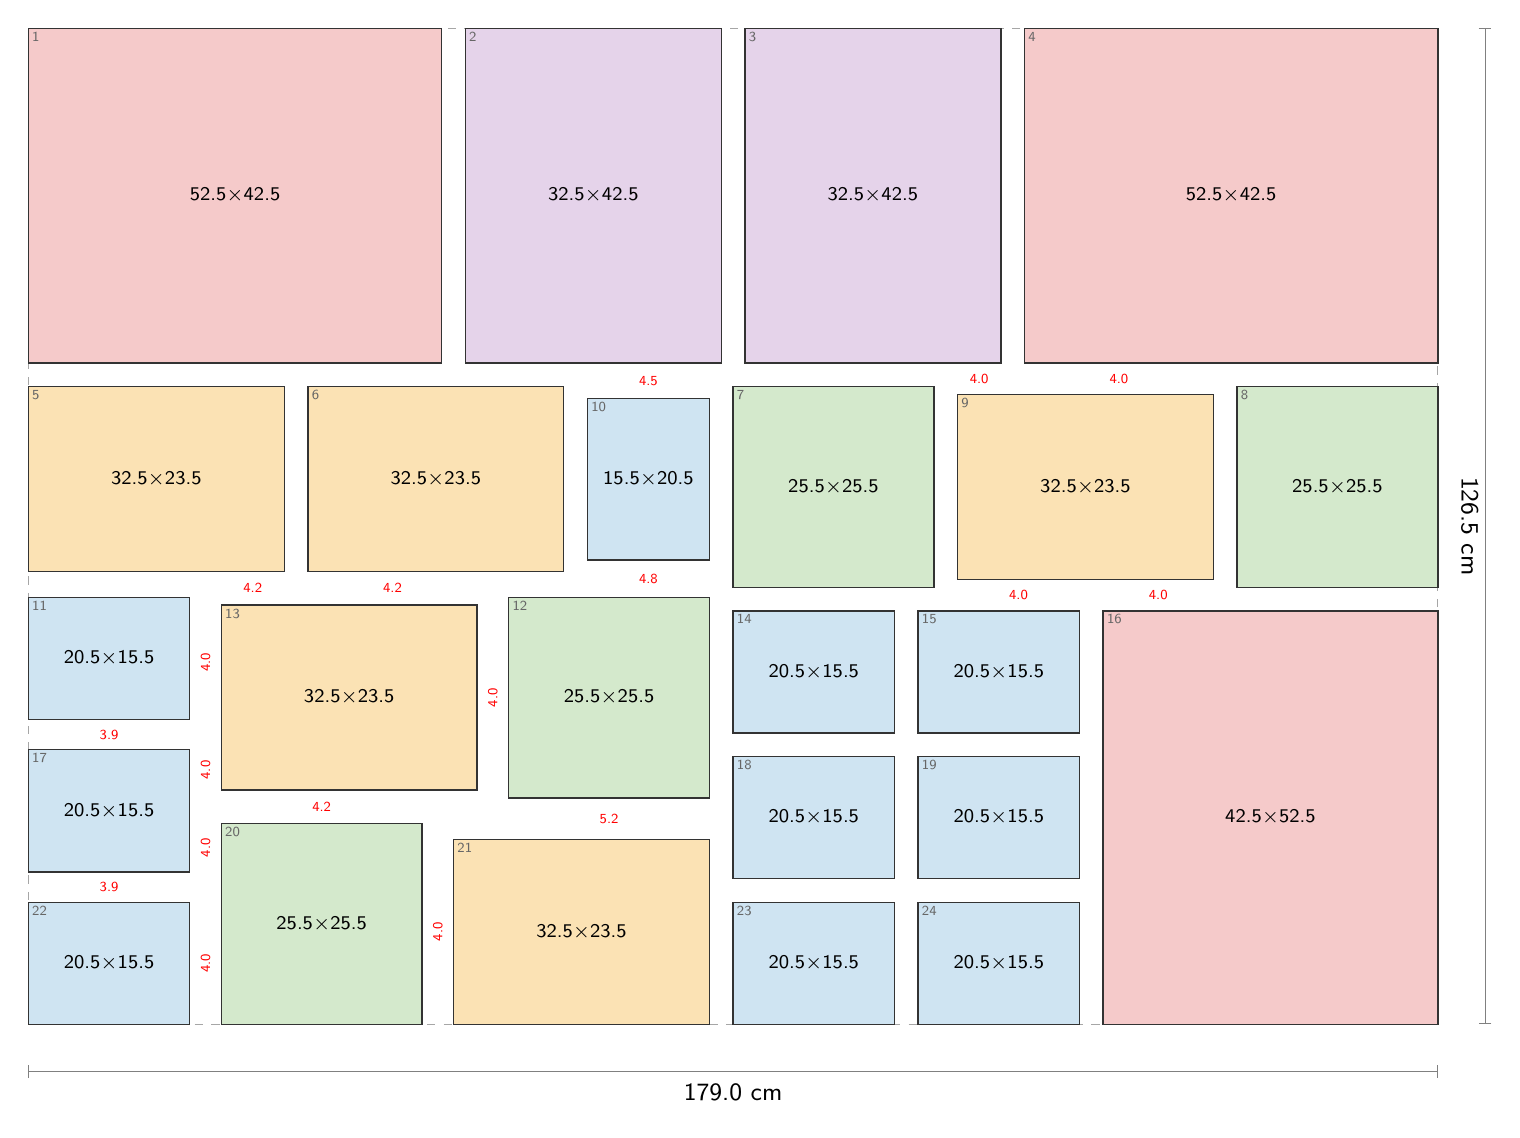
\begin{tikzpicture}[x=1mm, y=-1mm]
\draw[gray!70, dashed, line width=0.4pt] (0,0) rectangle (179.00,126.50);
\filldraw[fill=ft4, draw=black!80, line width=0.5pt] (0.00,0.00) rectangle (52.50,42.50);
\node[align=center, inner sep=0pt] at (26.25,21.25) {\scriptsize 52.5$\times$42.5};
\node[anchor=north west, inner sep=1.2pt, font=\tiny, text=black!60] at (0.00,0.00) {1};
\filldraw[fill=ft3, draw=black!80, line width=0.5pt] (55.50,0.00) rectangle (88.00,42.50);
\node[align=center, inner sep=0pt] at (71.75,21.25) {\scriptsize 32.5$\times$42.5};
\node[anchor=north west, inner sep=1.2pt, font=\tiny, text=black!60] at (55.50,0.00) {2};
\filldraw[fill=ft3, draw=black!80, line width=0.5pt] (91.00,0.00) rectangle (123.50,42.50);
\node[align=center, inner sep=0pt] at (107.25,21.25) {\scriptsize 32.5$\times$42.5};
\node[anchor=north west, inner sep=1.2pt, font=\tiny, text=black!60] at (91.00,0.00) {3};
\filldraw[fill=ft4, draw=black!80, line width=0.5pt] (126.50,0.00) rectangle (179.00,42.50);
\node[align=center, inner sep=0pt] at (152.75,21.25) {\scriptsize 52.5$\times$42.5};
\node[anchor=north west, inner sep=1.2pt, font=\tiny, text=black!60] at (126.50,0.00) {4};
\filldraw[fill=ft1, draw=black!80, line width=0.5pt] (0.00,45.50) rectangle (32.50,69.00);
\node[align=center, inner sep=0pt] at (16.25,57.25) {\scriptsize 32.5$\times$23.5};
\node[anchor=north west, inner sep=1.2pt, font=\tiny, text=black!60] at (0.00,45.50) {5};
\filldraw[fill=ft1, draw=black!80, line width=0.5pt] (35.50,45.50) rectangle (68.00,69.00);
\node[align=center, inner sep=0pt] at (51.75,57.25) {\scriptsize 32.5$\times$23.5};
\node[anchor=north west, inner sep=1.2pt, font=\tiny, text=black!60] at (35.50,45.50) {6};
\filldraw[fill=ft2, draw=black!80, line width=0.5pt] (89.50,45.50) rectangle (115.00,71.00);
\node[align=center, inner sep=0pt] at (102.25,58.25) {\scriptsize 25.5$\times$25.5};
\node[anchor=north west, inner sep=1.2pt, font=\tiny, text=black!60] at (89.50,45.50) {7};
\filldraw[fill=ft2, draw=black!80, line width=0.5pt] (153.50,45.50) rectangle (179.00,71.00);
\node[align=center, inner sep=0pt] at (166.25,58.25) {\scriptsize 25.5$\times$25.5};
\node[anchor=north west, inner sep=1.2pt, font=\tiny, text=black!60] at (153.50,45.50) {8};
\filldraw[fill=ft1, draw=black!80, line width=0.5pt] (118.00,46.50) rectangle (150.50,70.00);
\node[align=center, inner sep=0pt] at (134.25,58.25) {\scriptsize 32.5$\times$23.5};
\node[anchor=north west, inner sep=1.2pt, font=\tiny, text=black!60] at (118.00,46.50) {9};
\filldraw[fill=ft0, draw=black!80, line width=0.5pt] (71.00,47.00) rectangle (86.50,67.50);
\node[align=center, inner sep=0pt] at (78.75,57.25) {\scriptsize 15.5$\times$20.5};
\node[anchor=north west, inner sep=1.2pt, font=\tiny, text=black!60] at (71.00,47.00) {10};
\filldraw[fill=ft0, draw=black!80, line width=0.5pt] (0.00,72.25) rectangle (20.50,87.75);
\node[align=center, inner sep=0pt] at (10.25,80.00) {\scriptsize 20.5$\times$15.5};
\node[anchor=north west, inner sep=1.2pt, font=\tiny, text=black!60] at (0.00,72.25) {11};
\filldraw[fill=ft2, draw=black!80, line width=0.5pt] (61.00,72.25) rectangle (86.50,97.75);
\node[align=center, inner sep=0pt] at (73.75,85.00) {\scriptsize 25.5$\times$25.5};
\node[anchor=north west, inner sep=1.2pt, font=\tiny, text=black!60] at (61.00,72.25) {12};
\filldraw[fill=ft1, draw=black!80, line width=0.5pt] (24.50,73.25) rectangle (57.00,96.75);
\node[align=center, inner sep=0pt] at (40.75,85.00) {\scriptsize 32.5$\times$23.5};
\node[anchor=north west, inner sep=1.2pt, font=\tiny, text=black!60] at (24.50,73.25) {13};
\filldraw[fill=ft0, draw=black!80, line width=0.5pt] (89.50,74.00) rectangle (110.00,89.50);
\node[align=center, inner sep=0pt] at (99.75,81.75) {\scriptsize 20.5$\times$15.5};
\node[anchor=north west, inner sep=1.2pt, font=\tiny, text=black!60] at (89.50,74.00) {14};
\filldraw[fill=ft0, draw=black!80, line width=0.5pt] (113.00,74.00) rectangle (133.50,89.50);
\node[align=center, inner sep=0pt] at (123.25,81.75) {\scriptsize 20.5$\times$15.5};
\node[anchor=north west, inner sep=1.2pt, font=\tiny, text=black!60] at (113.00,74.00) {15};
\filldraw[fill=ft4, draw=black!80, line width=0.5pt] (136.50,74.00) rectangle (179.00,126.50);
\node[align=center, inner sep=0pt] at (157.75,100.25) {\scriptsize 42.5$\times$52.5};
\node[anchor=north west, inner sep=1.2pt, font=\tiny, text=black!60] at (136.50,74.00) {16};
\filldraw[fill=ft0, draw=black!80, line width=0.5pt] (0.00,91.62) rectangle (20.50,107.12);
\node[align=center, inner sep=0pt] at (10.25,99.38) {\scriptsize 20.5$\times$15.5};
\node[anchor=north west, inner sep=1.2pt, font=\tiny, text=black!60] at (0.00,91.62) {17};
\filldraw[fill=ft0, draw=black!80, line width=0.5pt] (89.50,92.50) rectangle (110.00,108.00);
\node[align=center, inner sep=0pt] at (99.75,100.25) {\scriptsize 20.5$\times$15.5};
\node[anchor=north west, inner sep=1.2pt, font=\tiny, text=black!60] at (89.50,92.50) {18};
\filldraw[fill=ft0, draw=black!80, line width=0.5pt] (113.00,92.50) rectangle (133.50,108.00);
\node[align=center, inner sep=0pt] at (123.25,100.25) {\scriptsize 20.5$\times$15.5};
\node[anchor=north west, inner sep=1.2pt, font=\tiny, text=black!60] at (113.00,92.50) {19};
\filldraw[fill=ft2, draw=black!80, line width=0.5pt] (24.50,101.00) rectangle (50.00,126.50);
\node[align=center, inner sep=0pt] at (37.25,113.75) {\scriptsize 25.5$\times$25.5};
\node[anchor=north west, inner sep=1.2pt, font=\tiny, text=black!60] at (24.50,101.00) {20};
\filldraw[fill=ft1, draw=black!80, line width=0.5pt] (54.00,103.00) rectangle (86.50,126.50);
\node[align=center, inner sep=0pt] at (70.25,114.75) {\scriptsize 32.5$\times$23.5};
\node[anchor=north west, inner sep=1.2pt, font=\tiny, text=black!60] at (54.00,103.00) {21};
\filldraw[fill=ft0, draw=black!80, line width=0.5pt] (0.00,111.00) rectangle (20.50,126.50);
\node[align=center, inner sep=0pt] at (10.25,118.75) {\scriptsize 20.5$\times$15.5};
\node[anchor=north west, inner sep=1.2pt, font=\tiny, text=black!60] at (0.00,111.00) {22};
\filldraw[fill=ft0, draw=black!80, line width=0.5pt] (89.50,111.00) rectangle (110.00,126.50);
\node[align=center, inner sep=0pt] at (99.75,118.75) {\scriptsize 20.5$\times$15.5};
\node[anchor=north west, inner sep=1.2pt, font=\tiny, text=black!60] at (89.50,111.00) {23};
\filldraw[fill=ft0, draw=black!80, line width=0.5pt] (113.00,111.00) rectangle (133.50,126.50);
\node[align=center, inner sep=0pt] at (123.25,118.75) {\scriptsize 20.5$\times$15.5};
\node[anchor=north west, inner sep=1.2pt, font=\tiny, text=black!60] at (113.00,111.00) {24};
\node[font=\tiny, text=red, fill=white, inner sep=0.3pt] at (78.75,44.75) {4.5};
\node[font=\tiny, text=red, fill=white, inner sep=0.3pt] at (120.75,44.50) {4.0};
\node[font=\tiny, text=red, fill=white, inner sep=0.3pt] at (138.50,44.50) {4.0};
\node[font=\tiny, text=red, fill=white, inner sep=0.3pt] at (28.50,71.12) {4.2};
\node[font=\tiny, text=red, fill=white, inner sep=0.3pt] at (46.25,71.12) {4.2};
\node[font=\tiny, text=red, fill=white, inner sep=0.3pt] at (125.75,72.00) {4.0};
\node[font=\tiny, text=red, fill=white, inner sep=0.3pt] at (143.50,72.00) {4.0};
\node[font=\tiny, text=red, fill=white, inner sep=0.3pt] at (78.75,69.88) {4.8};
\node[font=\tiny, text=red, fill=white, inner sep=0.3pt, rotate=90] at (22.50,80.50) {4.0};
\node[font=\tiny, text=red, fill=white, inner sep=0.3pt] at (10.25,89.69) {3.9};
\node[font=\tiny, text=red, fill=white, inner sep=0.3pt] at (73.75,100.38) {5.2};
\node[font=\tiny, text=red, fill=white, inner sep=0.3pt, rotate=90] at (59.00,85.00) {4.0};
\node[font=\tiny, text=red, fill=white, inner sep=0.3pt] at (37.25,98.88) {4.2};
\node[font=\tiny, text=red, fill=white, inner sep=0.3pt, rotate=90] at (22.50,94.19) {4.0};
\node[font=\tiny, text=red, fill=white, inner sep=0.3pt, rotate=90] at (22.50,104.06) {4.0};
\node[font=\tiny, text=red, fill=white, inner sep=0.3pt] at (10.25,109.06) {3.9};
\node[font=\tiny, text=red, fill=white, inner sep=0.3pt, rotate=90] at (52.00,114.75) {4.0};
\node[font=\tiny, text=red, fill=white, inner sep=0.3pt, rotate=90] at (22.50,118.75) {4.0};
\draw[Bar-Bar, gray] (0,132.50) -- (179.00,132.50) node[midway, below=1pt, font=\small, text=black] {179.0 cm};
\draw[Bar-Bar, gray] (185.00,0) -- (185.00,126.50) node[midway, right=1pt, font=\small, text=black, rotate=-90, anchor=north] {126.5 cm};
\end{tikzpicture}\\[4pt]
{\scriptsize Scale 1:10 (1 mm = 1 cm). Red numbers mark gaps that deviate from the nominal gap by more than 0.25 cm. Small grey numbers index the coordinate table.}
\end{minipage}\hfill
\begin{minipage}[t]{0.25\textwidth}\vspace{0pt}
\small
\begin{tabular}{@{}l l@{}}
\toprule
Outer size & 179.0 $\times$ 126.5 cm \\
Nominal gap & 3 cm \\
Actual gaps & 3.0 -- 5.2 cm \\
Max.\ deviation & 2.2 cm \\
Mean deviation & 0.44 cm \\
Border notches & none \\
Corners filled & 4 / 4 \\
Frames used & 24 of 28 \\
\bottomrule
\end{tabular}

\vspace{8pt}
\scriptsize
\begin{tabular}{@{}c l l r r@{}}
\toprule
 & outer w $\times$ h (cm) & & used & have \\
\midrule
\tikz[baseline=-0.6ex]\fill[ft0,draw=black!60] (0,0) rectangle (1.2ex,1.2ex); & 20.5$\times$15.5 & L & 9 & 9 \\
\tikz[baseline=-0.6ex]\fill[ft0,draw=black!60] (0,0) rectangle (1.2ex,1.2ex); & 15.5$\times$20.5 & P & 1 & 2 \\
\tikz[baseline=-0.6ex]\fill[ft3,draw=black!60] (0,0) rectangle (1.2ex,1.2ex); & 32.5$\times$42.5 & P & 2 & 2 \\
\tikz[baseline=-0.6ex]\fill[ft3,draw=black!60] (0,0) rectangle (1.2ex,1.2ex); & 42.5$\times$32.5 & L & 0 & 1 \\
\tikz[baseline=-0.6ex]\fill[ft1,draw=black!60] (0,0) rectangle (1.2ex,1.2ex); & 32.5$\times$23.5 & L & 5 & 5 \\
\tikz[baseline=-0.6ex]\fill[ft1,draw=black!60] (0,0) rectangle (1.2ex,1.2ex); & 23.5$\times$32.5 & P & 0 & 1 \\
\tikz[baseline=-0.6ex]\fill[ft2,draw=black!60] (0,0) rectangle (1.2ex,1.2ex); & 25.5$\times$25.5 &  & 4 & 5 \\
\tikz[baseline=-0.6ex]\fill[ft4,draw=black!60] (0,0) rectangle (1.2ex,1.2ex); & 42.5$\times$52.5 & P & 1 & 1 \\
\tikz[baseline=-0.6ex]\fill[ft4,draw=black!60] (0,0) rectangle (1.2ex,1.2ex); & 52.5$\times$42.5 & L & 2 & 2 \\
\bottomrule
\end{tabular}

\vspace{8pt}
{\bfseries Positions} (top-left corner, cm)\\[2pt]
\tiny
\begin{tabular}{@{}r l r r@{}}
\toprule
\# & frame w $\times$ h & x & y \\
\midrule
1 & 52.5 $\times$ 42.5 & 0.0 & 0.0 \\
2 & 32.5 $\times$ 42.5 & 55.5 & 0.0 \\
3 & 32.5 $\times$ 42.5 & 91.0 & 0.0 \\
4 & 52.5 $\times$ 42.5 & 126.5 & 0.0 \\
5 & 32.5 $\times$ 23.5 & 0.0 & 45.5 \\
6 & 32.5 $\times$ 23.5 & 35.5 & 45.5 \\
7 & 25.5 $\times$ 25.5 & 89.5 & 45.5 \\
8 & 25.5 $\times$ 25.5 & 153.5 & 45.5 \\
9 & 32.5 $\times$ 23.5 & 118.0 & 46.5 \\
10 & 15.5 $\times$ 20.5 & 71.0 & 47.0 \\
11 & 20.5 $\times$ 15.5 & 0.0 & 72.2 \\
12 & 25.5 $\times$ 25.5 & 61.0 & 72.2 \\
13 & 32.5 $\times$ 23.5 & 24.5 & 73.2 \\
14 & 20.5 $\times$ 15.5 & 89.5 & 74.0 \\
15 & 20.5 $\times$ 15.5 & 113.0 & 74.0 \\
16 & 42.5 $\times$ 52.5 & 136.5 & 74.0 \\
17 & 20.5 $\times$ 15.5 & 0.0 & 91.6 \\
18 & 20.5 $\times$ 15.5 & 89.5 & 92.5 \\
19 & 20.5 $\times$ 15.5 & 113.0 & 92.5 \\
20 & 25.5 $\times$ 25.5 & 24.5 & 101.0 \\
21 & 32.5 $\times$ 23.5 & 54.0 & 103.0 \\
22 & 20.5 $\times$ 15.5 & 0.0 & 111.0 \\
23 & 20.5 $\times$ 15.5 & 89.5 & 111.0 \\
24 & 20.5 $\times$ 15.5 & 113.0 & 111.0 \\
\bottomrule
\end{tabular}
\end{minipage}
\clearpage

\begin{minipage}[t]{0.74\textwidth}\vspace{0pt}
{\LARGE\bfseries Layout 2}\hspace{1.5em}{\large 180.0 $\times$ 128.0 cm \quad gap 3 cm \quad 25 frames}\\[8pt]
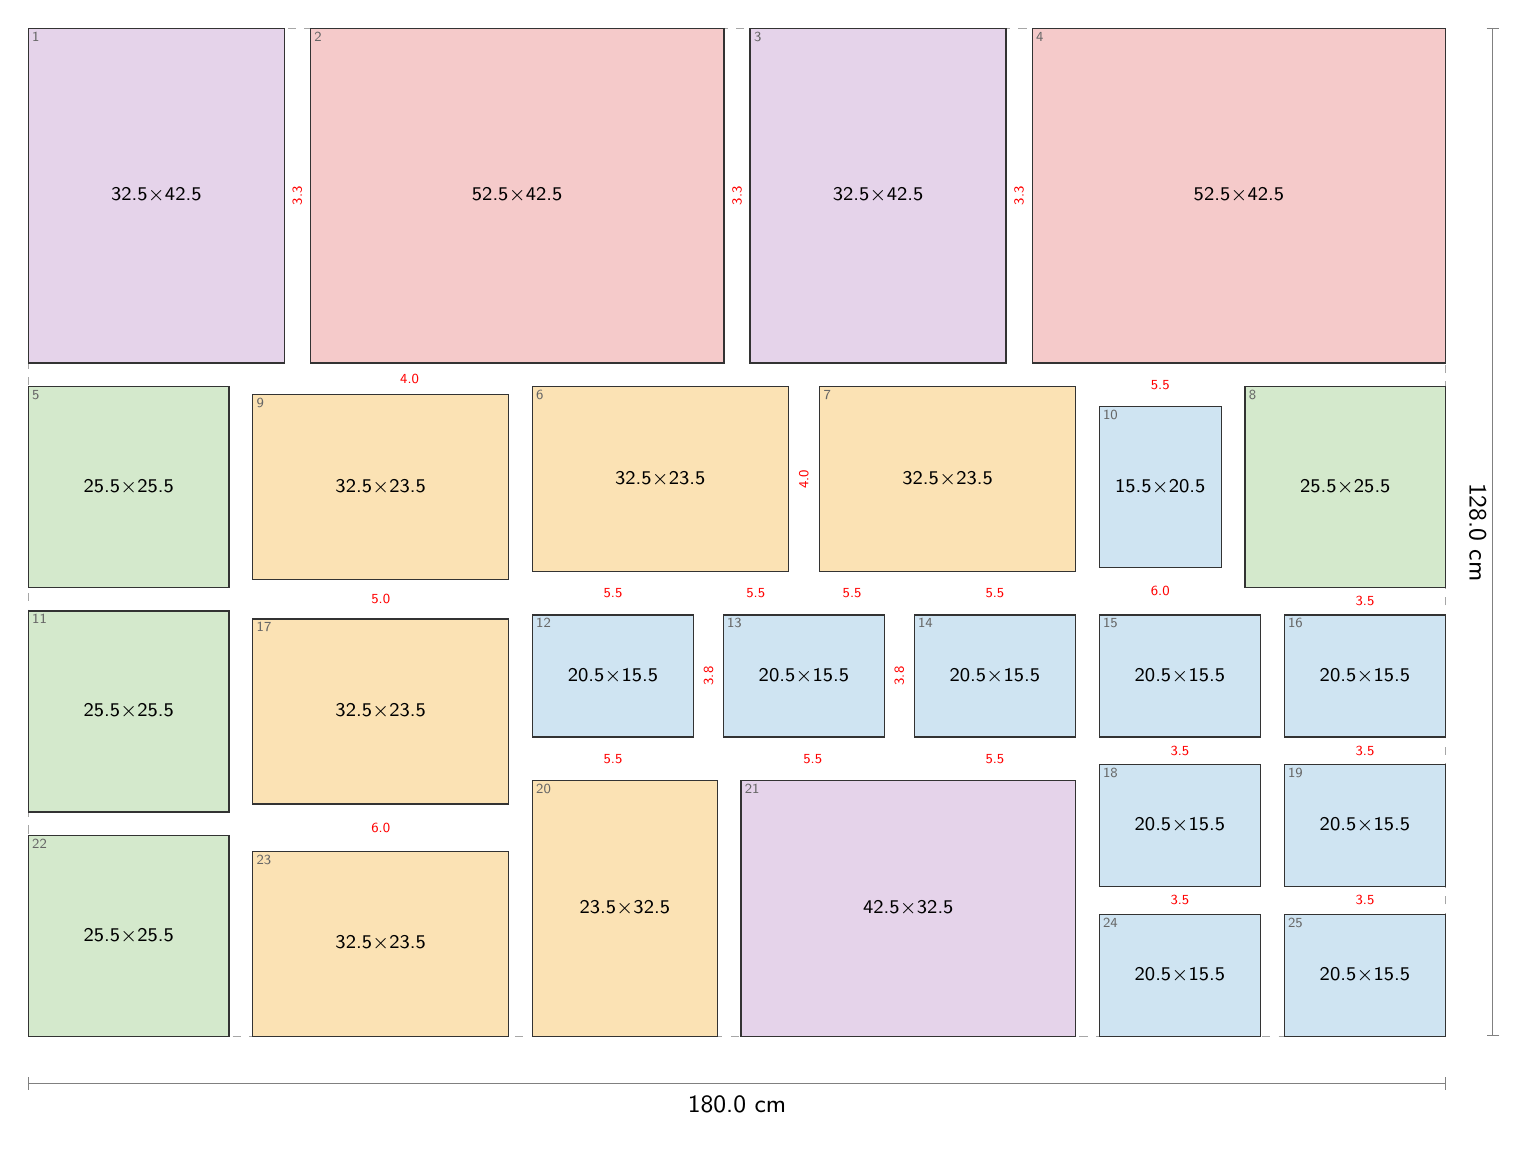
\begin{tikzpicture}[x=1mm, y=-1mm]
\draw[gray!70, dashed, line width=0.4pt] (0,0) rectangle (180.00,128.00);
\filldraw[fill=ft3, draw=black!80, line width=0.5pt] (0.00,0.00) rectangle (32.50,42.50);
\node[align=center, inner sep=0pt] at (16.25,21.25) {\scriptsize 32.5$\times$42.5};
\node[anchor=north west, inner sep=1.2pt, font=\tiny, text=black!60] at (0.00,0.00) {1};
\filldraw[fill=ft4, draw=black!80, line width=0.5pt] (35.83,0.00) rectangle (88.33,42.50);
\node[align=center, inner sep=0pt] at (62.08,21.25) {\scriptsize 52.5$\times$42.5};
\node[anchor=north west, inner sep=1.2pt, font=\tiny, text=black!60] at (35.83,0.00) {2};
\filldraw[fill=ft3, draw=black!80, line width=0.5pt] (91.67,0.00) rectangle (124.17,42.50);
\node[align=center, inner sep=0pt] at (107.92,21.25) {\scriptsize 32.5$\times$42.5};
\node[anchor=north west, inner sep=1.2pt, font=\tiny, text=black!60] at (91.67,0.00) {3};
\filldraw[fill=ft4, draw=black!80, line width=0.5pt] (127.50,0.00) rectangle (180.00,42.50);
\node[align=center, inner sep=0pt] at (153.75,21.25) {\scriptsize 52.5$\times$42.5};
\node[anchor=north west, inner sep=1.2pt, font=\tiny, text=black!60] at (127.50,0.00) {4};
\filldraw[fill=ft2, draw=black!80, line width=0.5pt] (0.00,45.50) rectangle (25.50,71.00);
\node[align=center, inner sep=0pt] at (12.75,58.25) {\scriptsize 25.5$\times$25.5};
\node[anchor=north west, inner sep=1.2pt, font=\tiny, text=black!60] at (0.00,45.50) {5};
\filldraw[fill=ft1, draw=black!80, line width=0.5pt] (64.00,45.50) rectangle (96.50,69.00);
\node[align=center, inner sep=0pt] at (80.25,57.25) {\scriptsize 32.5$\times$23.5};
\node[anchor=north west, inner sep=1.2pt, font=\tiny, text=black!60] at (64.00,45.50) {6};
\filldraw[fill=ft1, draw=black!80, line width=0.5pt] (100.50,45.50) rectangle (133.00,69.00);
\node[align=center, inner sep=0pt] at (116.75,57.25) {\scriptsize 32.5$\times$23.5};
\node[anchor=north west, inner sep=1.2pt, font=\tiny, text=black!60] at (100.50,45.50) {7};
\filldraw[fill=ft2, draw=black!80, line width=0.5pt] (154.50,45.50) rectangle (180.00,71.00);
\node[align=center, inner sep=0pt] at (167.25,58.25) {\scriptsize 25.5$\times$25.5};
\node[anchor=north west, inner sep=1.2pt, font=\tiny, text=black!60] at (154.50,45.50) {8};
\filldraw[fill=ft1, draw=black!80, line width=0.5pt] (28.50,46.50) rectangle (61.00,70.00);
\node[align=center, inner sep=0pt] at (44.75,58.25) {\scriptsize 32.5$\times$23.5};
\node[anchor=north west, inner sep=1.2pt, font=\tiny, text=black!60] at (28.50,46.50) {9};
\filldraw[fill=ft0, draw=black!80, line width=0.5pt] (136.00,48.00) rectangle (151.50,68.50);
\node[align=center, inner sep=0pt] at (143.75,58.25) {\scriptsize 15.5$\times$20.5};
\node[anchor=north west, inner sep=1.2pt, font=\tiny, text=black!60] at (136.00,48.00) {10};
\filldraw[fill=ft2, draw=black!80, line width=0.5pt] (0.00,74.00) rectangle (25.50,99.50);
\node[align=center, inner sep=0pt] at (12.75,86.75) {\scriptsize 25.5$\times$25.5};
\node[anchor=north west, inner sep=1.2pt, font=\tiny, text=black!60] at (0.00,74.00) {11};
\filldraw[fill=ft0, draw=black!80, line width=0.5pt] (64.00,74.50) rectangle (84.50,90.00);
\node[align=center, inner sep=0pt] at (74.25,82.25) {\scriptsize 20.5$\times$15.5};
\node[anchor=north west, inner sep=1.2pt, font=\tiny, text=black!60] at (64.00,74.50) {12};
\filldraw[fill=ft0, draw=black!80, line width=0.5pt] (88.25,74.50) rectangle (108.75,90.00);
\node[align=center, inner sep=0pt] at (98.50,82.25) {\scriptsize 20.5$\times$15.5};
\node[anchor=north west, inner sep=1.2pt, font=\tiny, text=black!60] at (88.25,74.50) {13};
\filldraw[fill=ft0, draw=black!80, line width=0.5pt] (112.50,74.50) rectangle (133.00,90.00);
\node[align=center, inner sep=0pt] at (122.75,82.25) {\scriptsize 20.5$\times$15.5};
\node[anchor=north west, inner sep=1.2pt, font=\tiny, text=black!60] at (112.50,74.50) {14};
\filldraw[fill=ft0, draw=black!80, line width=0.5pt] (136.00,74.50) rectangle (156.50,90.00);
\node[align=center, inner sep=0pt] at (146.25,82.25) {\scriptsize 20.5$\times$15.5};
\node[anchor=north west, inner sep=1.2pt, font=\tiny, text=black!60] at (136.00,74.50) {15};
\filldraw[fill=ft0, draw=black!80, line width=0.5pt] (159.50,74.50) rectangle (180.00,90.00);
\node[align=center, inner sep=0pt] at (169.75,82.25) {\scriptsize 20.5$\times$15.5};
\node[anchor=north west, inner sep=1.2pt, font=\tiny, text=black!60] at (159.50,74.50) {16};
\filldraw[fill=ft1, draw=black!80, line width=0.5pt] (28.50,75.00) rectangle (61.00,98.50);
\node[align=center, inner sep=0pt] at (44.75,86.75) {\scriptsize 32.5$\times$23.5};
\node[anchor=north west, inner sep=1.2pt, font=\tiny, text=black!60] at (28.50,75.00) {17};
\filldraw[fill=ft0, draw=black!80, line width=0.5pt] (136.00,93.50) rectangle (156.50,109.00);
\node[align=center, inner sep=0pt] at (146.25,101.25) {\scriptsize 20.5$\times$15.5};
\node[anchor=north west, inner sep=1.2pt, font=\tiny, text=black!60] at (136.00,93.50) {18};
\filldraw[fill=ft0, draw=black!80, line width=0.5pt] (159.50,93.50) rectangle (180.00,109.00);
\node[align=center, inner sep=0pt] at (169.75,101.25) {\scriptsize 20.5$\times$15.5};
\node[anchor=north west, inner sep=1.2pt, font=\tiny, text=black!60] at (159.50,93.50) {19};
\filldraw[fill=ft1, draw=black!80, line width=0.5pt] (64.00,95.50) rectangle (87.50,128.00);
\node[align=center, inner sep=0pt] at (75.75,111.75) {\scriptsize 23.5$\times$32.5};
\node[anchor=north west, inner sep=1.2pt, font=\tiny, text=black!60] at (64.00,95.50) {20};
\filldraw[fill=ft3, draw=black!80, line width=0.5pt] (90.50,95.50) rectangle (133.00,128.00);
\node[align=center, inner sep=0pt] at (111.75,111.75) {\scriptsize 42.5$\times$32.5};
\node[anchor=north west, inner sep=1.2pt, font=\tiny, text=black!60] at (90.50,95.50) {21};
\filldraw[fill=ft2, draw=black!80, line width=0.5pt] (0.00,102.50) rectangle (25.50,128.00);
\node[align=center, inner sep=0pt] at (12.75,115.25) {\scriptsize 25.5$\times$25.5};
\node[anchor=north west, inner sep=1.2pt, font=\tiny, text=black!60] at (0.00,102.50) {22};
\filldraw[fill=ft1, draw=black!80, line width=0.5pt] (28.50,104.50) rectangle (61.00,128.00);
\node[align=center, inner sep=0pt] at (44.75,116.25) {\scriptsize 32.5$\times$23.5};
\node[anchor=north west, inner sep=1.2pt, font=\tiny, text=black!60] at (28.50,104.50) {23};
\filldraw[fill=ft0, draw=black!80, line width=0.5pt] (136.00,112.50) rectangle (156.50,128.00);
\node[align=center, inner sep=0pt] at (146.25,120.25) {\scriptsize 20.5$\times$15.5};
\node[anchor=north west, inner sep=1.2pt, font=\tiny, text=black!60] at (136.00,112.50) {24};
\filldraw[fill=ft0, draw=black!80, line width=0.5pt] (159.50,112.50) rectangle (180.00,128.00);
\node[align=center, inner sep=0pt] at (169.75,120.25) {\scriptsize 20.5$\times$15.5};
\node[anchor=north west, inner sep=1.2pt, font=\tiny, text=black!60] at (159.50,112.50) {25};
\node[font=\tiny, text=red, fill=white, inner sep=0.3pt, rotate=90] at (34.17,21.25) {3.3};
\node[font=\tiny, text=red, fill=white, inner sep=0.3pt, rotate=90] at (90.00,21.25) {3.3};
\node[font=\tiny, text=red, fill=white, inner sep=0.3pt] at (48.42,44.50) {4.0};
\node[font=\tiny, text=red, fill=white, inner sep=0.3pt, rotate=90] at (125.83,21.25) {3.3};
\node[font=\tiny, text=red, fill=white, inner sep=0.3pt] at (143.75,45.25) {5.5};
\node[font=\tiny, text=red, fill=white, inner sep=0.3pt, rotate=90] at (98.50,57.25) {4.0};
\node[font=\tiny, text=red, fill=white, inner sep=0.3pt] at (74.25,71.75) {5.5};
\node[font=\tiny, text=red, fill=white, inner sep=0.3pt] at (92.38,71.75) {5.5};
\node[font=\tiny, text=red, fill=white, inner sep=0.3pt] at (104.62,71.75) {5.5};
\node[font=\tiny, text=red, fill=white, inner sep=0.3pt] at (122.75,71.75) {5.5};
\node[font=\tiny, text=red, fill=white, inner sep=0.3pt] at (169.75,72.75) {3.5};
\node[font=\tiny, text=red, fill=white, inner sep=0.3pt] at (44.75,72.50) {5.0};
\node[font=\tiny, text=red, fill=white, inner sep=0.3pt] at (143.75,71.50) {6.0};
\node[font=\tiny, text=red, fill=white, inner sep=0.3pt, rotate=90] at (86.38,82.25) {3.8};
\node[font=\tiny, text=red, fill=white, inner sep=0.3pt] at (74.25,92.75) {5.5};
\node[font=\tiny, text=red, fill=white, inner sep=0.3pt, rotate=90] at (110.62,82.25) {3.8};
\node[font=\tiny, text=red, fill=white, inner sep=0.3pt] at (99.62,92.75) {5.5};
\node[font=\tiny, text=red, fill=white, inner sep=0.3pt] at (122.75,92.75) {5.5};
\node[font=\tiny, text=red, fill=white, inner sep=0.3pt] at (146.25,91.75) {3.5};
\node[font=\tiny, text=red, fill=white, inner sep=0.3pt] at (169.75,91.75) {3.5};
\node[font=\tiny, text=red, fill=white, inner sep=0.3pt] at (44.75,101.50) {6.0};
\node[font=\tiny, text=red, fill=white, inner sep=0.3pt] at (146.25,110.75) {3.5};
\node[font=\tiny, text=red, fill=white, inner sep=0.3pt] at (169.75,110.75) {3.5};
\draw[Bar-Bar, gray] (0,134.00) -- (180.00,134.00) node[midway, below=1pt, font=\small, text=black] {180.0 cm};
\draw[Bar-Bar, gray] (186.00,0) -- (186.00,128.00) node[midway, right=1pt, font=\small, text=black, rotate=-90, anchor=north] {128.0 cm};
\end{tikzpicture}\\[4pt]
{\scriptsize Scale 1:10 (1 mm = 1 cm). Red numbers mark gaps that deviate from the nominal gap by more than 0.25 cm. Small grey numbers index the coordinate table.}
\end{minipage}\hfill
\begin{minipage}[t]{0.25\textwidth}\vspace{0pt}
\small
\begin{tabular}{@{}l l@{}}
\toprule
Outer size & 180.0 $\times$ 128.0 cm \\
Nominal gap & 3 cm \\
Actual gaps & 3.0 -- 6.0 cm \\
Max.\ deviation & 3.0 cm \\
Mean deviation & 0.78 cm \\
Border notches & none \\
Corners filled & 4 / 4 \\
Frames used & 25 of 28 \\
\bottomrule
\end{tabular}

\vspace{8pt}
\scriptsize
\begin{tabular}{@{}c l l r r@{}}
\toprule
 & outer w $\times$ h (cm) & & used & have \\
\midrule
\tikz[baseline=-0.6ex]\fill[ft0,draw=black!60] (0,0) rectangle (1.2ex,1.2ex); & 20.5$\times$15.5 & L & 9 & 9 \\
\tikz[baseline=-0.6ex]\fill[ft0,draw=black!60] (0,0) rectangle (1.2ex,1.2ex); & 15.5$\times$20.5 & P & 1 & 2 \\
\tikz[baseline=-0.6ex]\fill[ft3,draw=black!60] (0,0) rectangle (1.2ex,1.2ex); & 32.5$\times$42.5 & P & 2 & 2 \\
\tikz[baseline=-0.6ex]\fill[ft3,draw=black!60] (0,0) rectangle (1.2ex,1.2ex); & 42.5$\times$32.5 & L & 1 & 1 \\
\tikz[baseline=-0.6ex]\fill[ft1,draw=black!60] (0,0) rectangle (1.2ex,1.2ex); & 32.5$\times$23.5 & L & 5 & 5 \\
\tikz[baseline=-0.6ex]\fill[ft1,draw=black!60] (0,0) rectangle (1.2ex,1.2ex); & 23.5$\times$32.5 & P & 1 & 1 \\
\tikz[baseline=-0.6ex]\fill[ft2,draw=black!60] (0,0) rectangle (1.2ex,1.2ex); & 25.5$\times$25.5 &  & 4 & 5 \\
\tikz[baseline=-0.6ex]\fill[ft4,draw=black!60] (0,0) rectangle (1.2ex,1.2ex); & 42.5$\times$52.5 & P & 0 & 1 \\
\tikz[baseline=-0.6ex]\fill[ft4,draw=black!60] (0,0) rectangle (1.2ex,1.2ex); & 52.5$\times$42.5 & L & 2 & 2 \\
\bottomrule
\end{tabular}

\vspace{8pt}
{\bfseries Positions} (top-left corner, cm)\\[2pt]
\tiny
\begin{tabular}{@{}r l r r@{}}
\toprule
\# & frame w $\times$ h & x & y \\
\midrule
1 & 32.5 $\times$ 42.5 & 0.0 & 0.0 \\
2 & 52.5 $\times$ 42.5 & 35.8 & 0.0 \\
3 & 32.5 $\times$ 42.5 & 91.7 & 0.0 \\
4 & 52.5 $\times$ 42.5 & 127.5 & 0.0 \\
5 & 25.5 $\times$ 25.5 & 0.0 & 45.5 \\
6 & 32.5 $\times$ 23.5 & 64.0 & 45.5 \\
7 & 32.5 $\times$ 23.5 & 100.5 & 45.5 \\
8 & 25.5 $\times$ 25.5 & 154.5 & 45.5 \\
9 & 32.5 $\times$ 23.5 & 28.5 & 46.5 \\
10 & 15.5 $\times$ 20.5 & 136.0 & 48.0 \\
11 & 25.5 $\times$ 25.5 & 0.0 & 74.0 \\
12 & 20.5 $\times$ 15.5 & 64.0 & 74.5 \\
13 & 20.5 $\times$ 15.5 & 88.2 & 74.5 \\
14 & 20.5 $\times$ 15.5 & 112.5 & 74.5 \\
15 & 20.5 $\times$ 15.5 & 136.0 & 74.5 \\
16 & 20.5 $\times$ 15.5 & 159.5 & 74.5 \\
17 & 32.5 $\times$ 23.5 & 28.5 & 75.0 \\
18 & 20.5 $\times$ 15.5 & 136.0 & 93.5 \\
19 & 20.5 $\times$ 15.5 & 159.5 & 93.5 \\
20 & 23.5 $\times$ 32.5 & 64.0 & 95.5 \\
21 & 42.5 $\times$ 32.5 & 90.5 & 95.5 \\
22 & 25.5 $\times$ 25.5 & 0.0 & 102.5 \\
23 & 32.5 $\times$ 23.5 & 28.5 & 104.5 \\
24 & 20.5 $\times$ 15.5 & 136.0 & 112.5 \\
25 & 20.5 $\times$ 15.5 & 159.5 & 112.5 \\
\bottomrule
\end{tabular}
\end{minipage}
\clearpage

\begin{minipage}[t]{0.74\textwidth}\vspace{0pt}
{\LARGE\bfseries Layout 3}\hspace{1.5em}{\large 175.0 $\times$ 118.0 cm \quad gap 3 cm \quad 24 frames}\\[8pt]
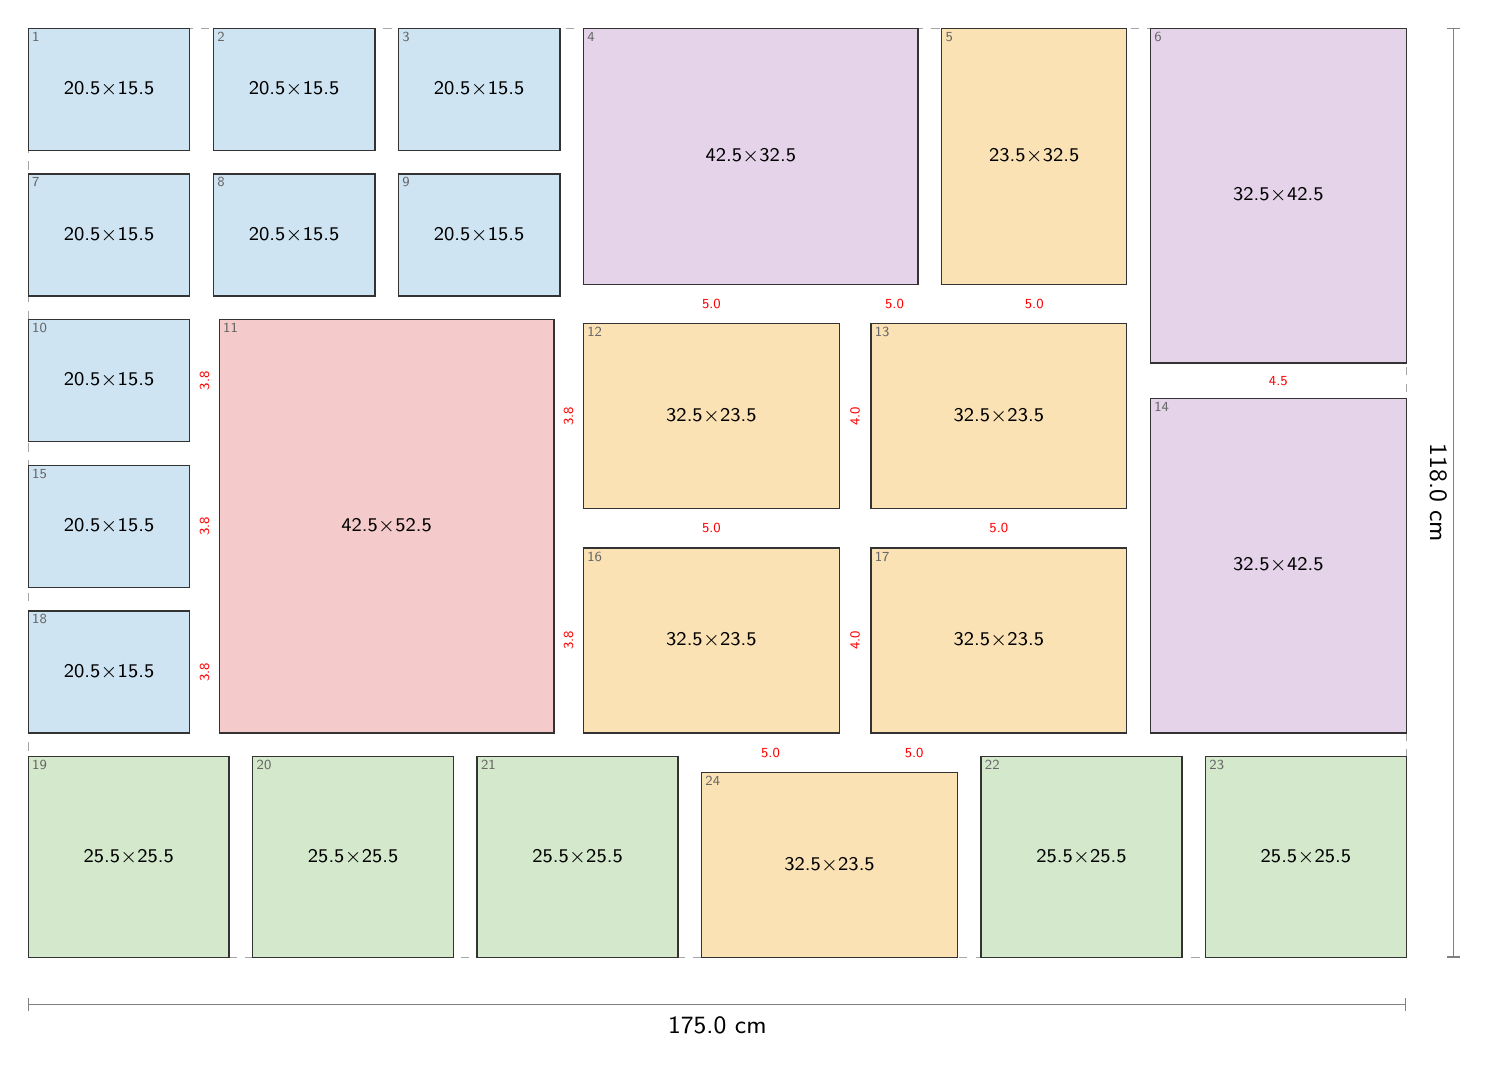
\begin{tikzpicture}[x=1mm, y=-1mm]
\draw[gray!70, dashed, line width=0.4pt] (0,0) rectangle (175.00,118.00);
\filldraw[fill=ft0, draw=black!80, line width=0.5pt] (0.00,0.00) rectangle (20.50,15.50);
\node[align=center, inner sep=0pt] at (10.25,7.75) {\scriptsize 20.5$\times$15.5};
\node[anchor=north west, inner sep=1.2pt, font=\tiny, text=black!60] at (0.00,0.00) {1};
\filldraw[fill=ft0, draw=black!80, line width=0.5pt] (23.50,0.00) rectangle (44.00,15.50);
\node[align=center, inner sep=0pt] at (33.75,7.75) {\scriptsize 20.5$\times$15.5};
\node[anchor=north west, inner sep=1.2pt, font=\tiny, text=black!60] at (23.50,0.00) {2};
\filldraw[fill=ft0, draw=black!80, line width=0.5pt] (47.00,0.00) rectangle (67.50,15.50);
\node[align=center, inner sep=0pt] at (57.25,7.75) {\scriptsize 20.5$\times$15.5};
\node[anchor=north west, inner sep=1.2pt, font=\tiny, text=black!60] at (47.00,0.00) {3};
\filldraw[fill=ft3, draw=black!80, line width=0.5pt] (70.50,0.00) rectangle (113.00,32.50);
\node[align=center, inner sep=0pt] at (91.75,16.25) {\scriptsize 42.5$\times$32.5};
\node[anchor=north west, inner sep=1.2pt, font=\tiny, text=black!60] at (70.50,0.00) {4};
\filldraw[fill=ft1, draw=black!80, line width=0.5pt] (116.00,0.00) rectangle (139.50,32.50);
\node[align=center, inner sep=0pt] at (127.75,16.25) {\scriptsize 23.5$\times$32.5};
\node[anchor=north west, inner sep=1.2pt, font=\tiny, text=black!60] at (116.00,0.00) {5};
\filldraw[fill=ft3, draw=black!80, line width=0.5pt] (142.50,0.00) rectangle (175.00,42.50);
\node[align=center, inner sep=0pt] at (158.75,21.25) {\scriptsize 32.5$\times$42.5};
\node[anchor=north west, inner sep=1.2pt, font=\tiny, text=black!60] at (142.50,0.00) {6};
\filldraw[fill=ft0, draw=black!80, line width=0.5pt] (0.00,18.50) rectangle (20.50,34.00);
\node[align=center, inner sep=0pt] at (10.25,26.25) {\scriptsize 20.5$\times$15.5};
\node[anchor=north west, inner sep=1.2pt, font=\tiny, text=black!60] at (0.00,18.50) {7};
\filldraw[fill=ft0, draw=black!80, line width=0.5pt] (23.50,18.50) rectangle (44.00,34.00);
\node[align=center, inner sep=0pt] at (33.75,26.25) {\scriptsize 20.5$\times$15.5};
\node[anchor=north west, inner sep=1.2pt, font=\tiny, text=black!60] at (23.50,18.50) {8};
\filldraw[fill=ft0, draw=black!80, line width=0.5pt] (47.00,18.50) rectangle (67.50,34.00);
\node[align=center, inner sep=0pt] at (57.25,26.25) {\scriptsize 20.5$\times$15.5};
\node[anchor=north west, inner sep=1.2pt, font=\tiny, text=black!60] at (47.00,18.50) {9};
\filldraw[fill=ft0, draw=black!80, line width=0.5pt] (0.00,37.00) rectangle (20.50,52.50);
\node[align=center, inner sep=0pt] at (10.25,44.75) {\scriptsize 20.5$\times$15.5};
\node[anchor=north west, inner sep=1.2pt, font=\tiny, text=black!60] at (0.00,37.00) {10};
\filldraw[fill=ft4, draw=black!80, line width=0.5pt] (24.25,37.00) rectangle (66.75,89.50);
\node[align=center, inner sep=0pt] at (45.50,63.25) {\scriptsize 42.5$\times$52.5};
\node[anchor=north west, inner sep=1.2pt, font=\tiny, text=black!60] at (24.25,37.00) {11};
\filldraw[fill=ft1, draw=black!80, line width=0.5pt] (70.50,37.50) rectangle (103.00,61.00);
\node[align=center, inner sep=0pt] at (86.75,49.25) {\scriptsize 32.5$\times$23.5};
\node[anchor=north west, inner sep=1.2pt, font=\tiny, text=black!60] at (70.50,37.50) {12};
\filldraw[fill=ft1, draw=black!80, line width=0.5pt] (107.00,37.50) rectangle (139.50,61.00);
\node[align=center, inner sep=0pt] at (123.25,49.25) {\scriptsize 32.5$\times$23.5};
\node[anchor=north west, inner sep=1.2pt, font=\tiny, text=black!60] at (107.00,37.50) {13};
\filldraw[fill=ft3, draw=black!80, line width=0.5pt] (142.50,47.00) rectangle (175.00,89.50);
\node[align=center, inner sep=0pt] at (158.75,68.25) {\scriptsize 32.5$\times$42.5};
\node[anchor=north west, inner sep=1.2pt, font=\tiny, text=black!60] at (142.50,47.00) {14};
\filldraw[fill=ft0, draw=black!80, line width=0.5pt] (0.00,55.50) rectangle (20.50,71.00);
\node[align=center, inner sep=0pt] at (10.25,63.25) {\scriptsize 20.5$\times$15.5};
\node[anchor=north west, inner sep=1.2pt, font=\tiny, text=black!60] at (0.00,55.50) {15};
\filldraw[fill=ft1, draw=black!80, line width=0.5pt] (70.50,66.00) rectangle (103.00,89.50);
\node[align=center, inner sep=0pt] at (86.75,77.75) {\scriptsize 32.5$\times$23.5};
\node[anchor=north west, inner sep=1.2pt, font=\tiny, text=black!60] at (70.50,66.00) {16};
\filldraw[fill=ft1, draw=black!80, line width=0.5pt] (107.00,66.00) rectangle (139.50,89.50);
\node[align=center, inner sep=0pt] at (123.25,77.75) {\scriptsize 32.5$\times$23.5};
\node[anchor=north west, inner sep=1.2pt, font=\tiny, text=black!60] at (107.00,66.00) {17};
\filldraw[fill=ft0, draw=black!80, line width=0.5pt] (0.00,74.00) rectangle (20.50,89.50);
\node[align=center, inner sep=0pt] at (10.25,81.75) {\scriptsize 20.5$\times$15.5};
\node[anchor=north west, inner sep=1.2pt, font=\tiny, text=black!60] at (0.00,74.00) {18};
\filldraw[fill=ft2, draw=black!80, line width=0.5pt] (0.00,92.50) rectangle (25.50,118.00);
\node[align=center, inner sep=0pt] at (12.75,105.25) {\scriptsize 25.5$\times$25.5};
\node[anchor=north west, inner sep=1.2pt, font=\tiny, text=black!60] at (0.00,92.50) {19};
\filldraw[fill=ft2, draw=black!80, line width=0.5pt] (28.50,92.50) rectangle (54.00,118.00);
\node[align=center, inner sep=0pt] at (41.25,105.25) {\scriptsize 25.5$\times$25.5};
\node[anchor=north west, inner sep=1.2pt, font=\tiny, text=black!60] at (28.50,92.50) {20};
\filldraw[fill=ft2, draw=black!80, line width=0.5pt] (57.00,92.50) rectangle (82.50,118.00);
\node[align=center, inner sep=0pt] at (69.75,105.25) {\scriptsize 25.5$\times$25.5};
\node[anchor=north west, inner sep=1.2pt, font=\tiny, text=black!60] at (57.00,92.50) {21};
\filldraw[fill=ft2, draw=black!80, line width=0.5pt] (121.00,92.50) rectangle (146.50,118.00);
\node[align=center, inner sep=0pt] at (133.75,105.25) {\scriptsize 25.5$\times$25.5};
\node[anchor=north west, inner sep=1.2pt, font=\tiny, text=black!60] at (121.00,92.50) {22};
\filldraw[fill=ft2, draw=black!80, line width=0.5pt] (149.50,92.50) rectangle (175.00,118.00);
\node[align=center, inner sep=0pt] at (162.25,105.25) {\scriptsize 25.5$\times$25.5};
\node[anchor=north west, inner sep=1.2pt, font=\tiny, text=black!60] at (149.50,92.50) {23};
\filldraw[fill=ft1, draw=black!80, line width=0.5pt] (85.50,94.50) rectangle (118.00,118.00);
\node[align=center, inner sep=0pt] at (101.75,106.25) {\scriptsize 32.5$\times$23.5};
\node[anchor=north west, inner sep=1.2pt, font=\tiny, text=black!60] at (85.50,94.50) {24};
\node[font=\tiny, text=red, fill=white, inner sep=0.3pt] at (86.75,35.00) {5.0};
\node[font=\tiny, text=red, fill=white, inner sep=0.3pt] at (110.00,35.00) {5.0};
\node[font=\tiny, text=red, fill=white, inner sep=0.3pt] at (127.75,35.00) {5.0};
\node[font=\tiny, text=red, fill=white, inner sep=0.3pt] at (158.75,44.75) {4.5};
\node[font=\tiny, text=red, fill=white, inner sep=0.3pt, rotate=90] at (22.38,44.75) {3.8};
\node[font=\tiny, text=red, fill=white, inner sep=0.3pt, rotate=90] at (68.62,49.25) {3.8};
\node[font=\tiny, text=red, fill=white, inner sep=0.3pt, rotate=90] at (68.62,77.75) {3.8};
\node[font=\tiny, text=red, fill=white, inner sep=0.3pt, rotate=90] at (105.00,49.25) {4.0};
\node[font=\tiny, text=red, fill=white, inner sep=0.3pt] at (86.75,63.50) {5.0};
\node[font=\tiny, text=red, fill=white, inner sep=0.3pt] at (123.25,63.50) {5.0};
\node[font=\tiny, text=red, fill=white, inner sep=0.3pt, rotate=90] at (22.38,63.25) {3.8};
\node[font=\tiny, text=red, fill=white, inner sep=0.3pt, rotate=90] at (105.00,77.75) {4.0};
\node[font=\tiny, text=red, fill=white, inner sep=0.3pt] at (94.25,92.00) {5.0};
\node[font=\tiny, text=red, fill=white, inner sep=0.3pt] at (112.50,92.00) {5.0};
\node[font=\tiny, text=red, fill=white, inner sep=0.3pt, rotate=90] at (22.38,81.75) {3.8};
\draw[Bar-Bar, gray] (0,124.00) -- (175.00,124.00) node[midway, below=1pt, font=\small, text=black] {175.0 cm};
\draw[Bar-Bar, gray] (181.00,0) -- (181.00,118.00) node[midway, right=1pt, font=\small, text=black, rotate=-90, anchor=north] {118.0 cm};
\end{tikzpicture}\\[4pt]
{\scriptsize Scale 1:10 (1 mm = 1 cm). Red numbers mark gaps that deviate from the nominal gap by more than 0.25 cm. Small grey numbers index the coordinate table.}
\end{minipage}\hfill
\begin{minipage}[t]{0.25\textwidth}\vspace{0pt}
\small
\begin{tabular}{@{}l l@{}}
\toprule
Outer size & 175.0 $\times$ 118.0 cm \\
Nominal gap & 3 cm \\
Actual gaps & 3.0 -- 5.0 cm \\
Max.\ deviation & 2.0 cm \\
Mean deviation & 0.47 cm \\
Border notches & right 4 cm \\
Corners filled & 4 / 4 \\
Frames used & 24 of 28 \\
\bottomrule
\end{tabular}

\vspace{8pt}
\scriptsize
\begin{tabular}{@{}c l l r r@{}}
\toprule
 & outer w $\times$ h (cm) & & used & have \\
\midrule
\tikz[baseline=-0.6ex]\fill[ft0,draw=black!60] (0,0) rectangle (1.2ex,1.2ex); & 20.5$\times$15.5 & L & 9 & 9 \\
\tikz[baseline=-0.6ex]\fill[ft0,draw=black!60] (0,0) rectangle (1.2ex,1.2ex); & 15.5$\times$20.5 & P & 0 & 2 \\
\tikz[baseline=-0.6ex]\fill[ft3,draw=black!60] (0,0) rectangle (1.2ex,1.2ex); & 32.5$\times$42.5 & P & 2 & 2 \\
\tikz[baseline=-0.6ex]\fill[ft3,draw=black!60] (0,0) rectangle (1.2ex,1.2ex); & 42.5$\times$32.5 & L & 1 & 1 \\
\tikz[baseline=-0.6ex]\fill[ft1,draw=black!60] (0,0) rectangle (1.2ex,1.2ex); & 32.5$\times$23.5 & L & 5 & 5 \\
\tikz[baseline=-0.6ex]\fill[ft1,draw=black!60] (0,0) rectangle (1.2ex,1.2ex); & 23.5$\times$32.5 & P & 1 & 1 \\
\tikz[baseline=-0.6ex]\fill[ft2,draw=black!60] (0,0) rectangle (1.2ex,1.2ex); & 25.5$\times$25.5 &  & 5 & 5 \\
\tikz[baseline=-0.6ex]\fill[ft4,draw=black!60] (0,0) rectangle (1.2ex,1.2ex); & 42.5$\times$52.5 & P & 1 & 1 \\
\tikz[baseline=-0.6ex]\fill[ft4,draw=black!60] (0,0) rectangle (1.2ex,1.2ex); & 52.5$\times$42.5 & L & 0 & 2 \\
\bottomrule
\end{tabular}

\vspace{8pt}
{\bfseries Positions} (top-left corner, cm)\\[2pt]
\tiny
\begin{tabular}{@{}r l r r@{}}
\toprule
\# & frame w $\times$ h & x & y \\
\midrule
1 & 20.5 $\times$ 15.5 & 0.0 & 0.0 \\
2 & 20.5 $\times$ 15.5 & 23.5 & 0.0 \\
3 & 20.5 $\times$ 15.5 & 47.0 & 0.0 \\
4 & 42.5 $\times$ 32.5 & 70.5 & 0.0 \\
5 & 23.5 $\times$ 32.5 & 116.0 & 0.0 \\
6 & 32.5 $\times$ 42.5 & 142.5 & 0.0 \\
7 & 20.5 $\times$ 15.5 & 0.0 & 18.5 \\
8 & 20.5 $\times$ 15.5 & 23.5 & 18.5 \\
9 & 20.5 $\times$ 15.5 & 47.0 & 18.5 \\
10 & 20.5 $\times$ 15.5 & 0.0 & 37.0 \\
11 & 42.5 $\times$ 52.5 & 24.2 & 37.0 \\
12 & 32.5 $\times$ 23.5 & 70.5 & 37.5 \\
13 & 32.5 $\times$ 23.5 & 107.0 & 37.5 \\
14 & 32.5 $\times$ 42.5 & 142.5 & 47.0 \\
15 & 20.5 $\times$ 15.5 & 0.0 & 55.5 \\
16 & 32.5 $\times$ 23.5 & 70.5 & 66.0 \\
17 & 32.5 $\times$ 23.5 & 107.0 & 66.0 \\
18 & 20.5 $\times$ 15.5 & 0.0 & 74.0 \\
19 & 25.5 $\times$ 25.5 & 0.0 & 92.5 \\
20 & 25.5 $\times$ 25.5 & 28.5 & 92.5 \\
21 & 25.5 $\times$ 25.5 & 57.0 & 92.5 \\
22 & 25.5 $\times$ 25.5 & 121.0 & 92.5 \\
23 & 25.5 $\times$ 25.5 & 149.5 & 92.5 \\
24 & 32.5 $\times$ 23.5 & 85.5 & 94.5 \\
\bottomrule
\end{tabular}
\end{minipage}
\clearpage

\begin{minipage}[t]{0.74\textwidth}\vspace{0pt}
{\LARGE\bfseries Layout 4}\hspace{1.5em}{\large 188.5 $\times$ 116.5 cm \quad gap 3 cm \quad 24 frames}\\[8pt]
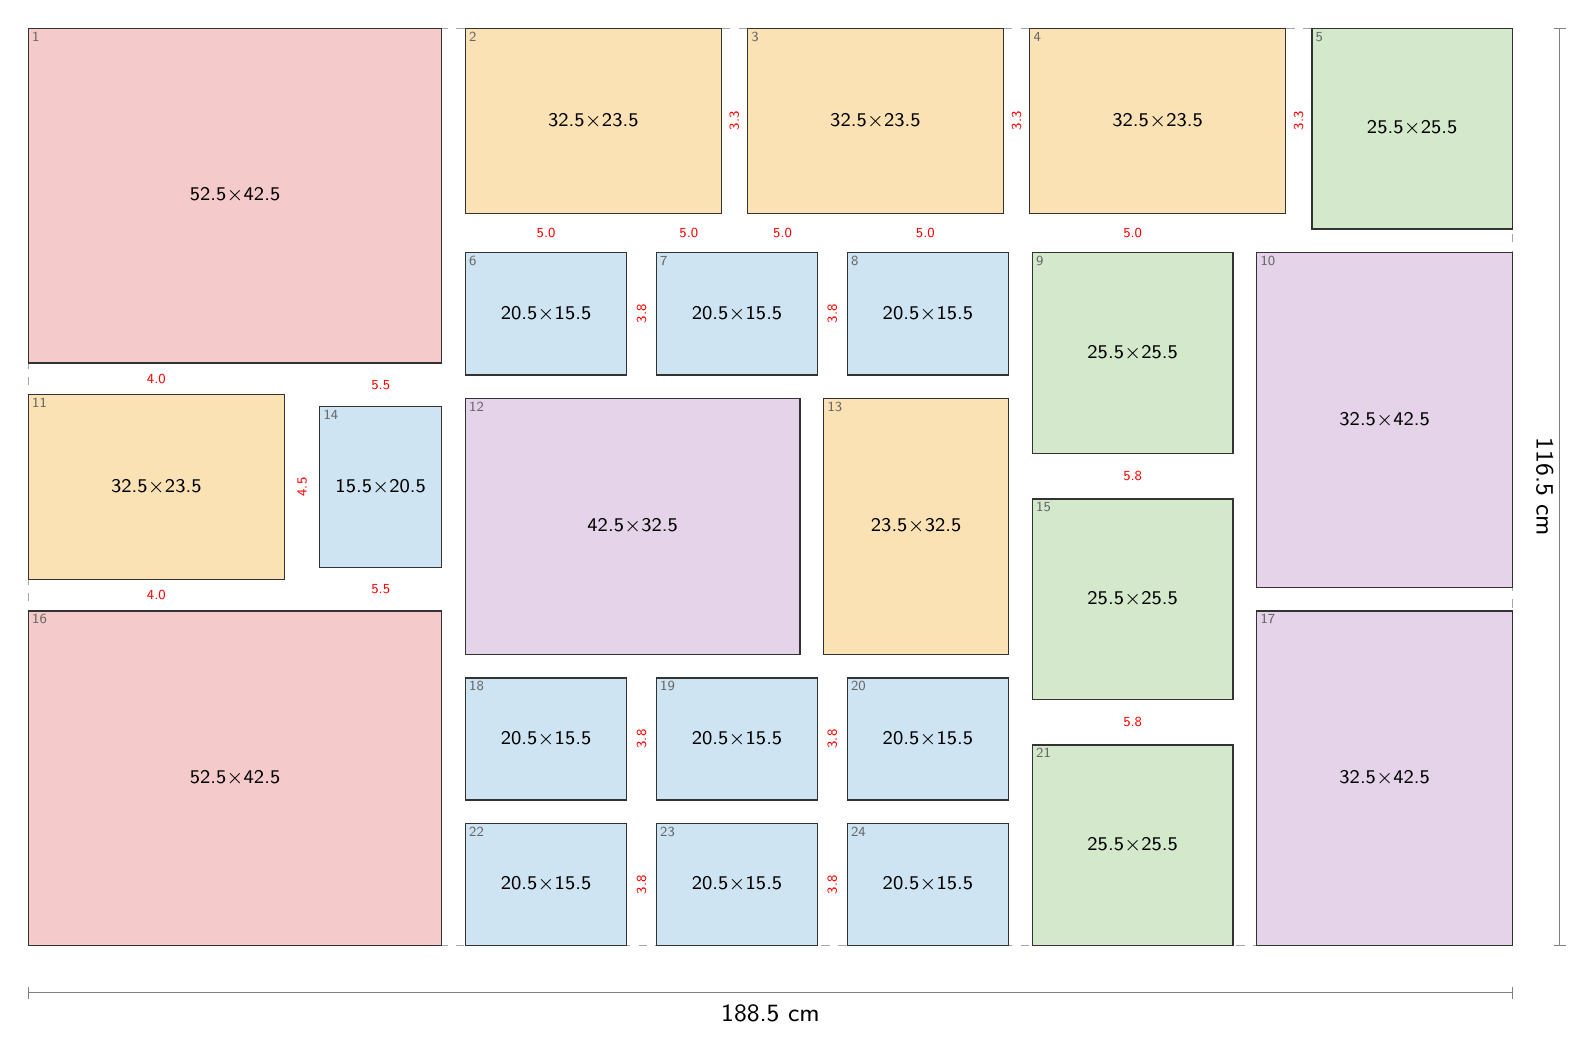
\begin{tikzpicture}[x=1mm, y=-1mm]
\draw[gray!70, dashed, line width=0.4pt] (0,0) rectangle (188.50,116.50);
\filldraw[fill=ft4, draw=black!80, line width=0.5pt] (0.00,0.00) rectangle (52.50,42.50);
\node[align=center, inner sep=0pt] at (26.25,21.25) {\scriptsize 52.5$\times$42.5};
\node[anchor=north west, inner sep=1.2pt, font=\tiny, text=black!60] at (0.00,0.00) {1};
\filldraw[fill=ft1, draw=black!80, line width=0.5pt] (55.50,0.00) rectangle (88.00,23.50);
\node[align=center, inner sep=0pt] at (71.75,11.75) {\scriptsize 32.5$\times$23.5};
\node[anchor=north west, inner sep=1.2pt, font=\tiny, text=black!60] at (55.50,0.00) {2};
\filldraw[fill=ft1, draw=black!80, line width=0.5pt] (91.33,0.00) rectangle (123.83,23.50);
\node[align=center, inner sep=0pt] at (107.58,11.75) {\scriptsize 32.5$\times$23.5};
\node[anchor=north west, inner sep=1.2pt, font=\tiny, text=black!60] at (91.33,0.00) {3};
\filldraw[fill=ft1, draw=black!80, line width=0.5pt] (127.17,0.00) rectangle (159.67,23.50);
\node[align=center, inner sep=0pt] at (143.42,11.75) {\scriptsize 32.5$\times$23.5};
\node[anchor=north west, inner sep=1.2pt, font=\tiny, text=black!60] at (127.17,0.00) {4};
\filldraw[fill=ft2, draw=black!80, line width=0.5pt] (163.00,0.00) rectangle (188.50,25.50);
\node[align=center, inner sep=0pt] at (175.75,12.75) {\scriptsize 25.5$\times$25.5};
\node[anchor=north west, inner sep=1.2pt, font=\tiny, text=black!60] at (163.00,0.00) {5};
\filldraw[fill=ft0, draw=black!80, line width=0.5pt] (55.50,28.50) rectangle (76.00,44.00);
\node[align=center, inner sep=0pt] at (65.75,36.25) {\scriptsize 20.5$\times$15.5};
\node[anchor=north west, inner sep=1.2pt, font=\tiny, text=black!60] at (55.50,28.50) {6};
\filldraw[fill=ft0, draw=black!80, line width=0.5pt] (79.75,28.50) rectangle (100.25,44.00);
\node[align=center, inner sep=0pt] at (90.00,36.25) {\scriptsize 20.5$\times$15.5};
\node[anchor=north west, inner sep=1.2pt, font=\tiny, text=black!60] at (79.75,28.50) {7};
\filldraw[fill=ft0, draw=black!80, line width=0.5pt] (104.00,28.50) rectangle (124.50,44.00);
\node[align=center, inner sep=0pt] at (114.25,36.25) {\scriptsize 20.5$\times$15.5};
\node[anchor=north west, inner sep=1.2pt, font=\tiny, text=black!60] at (104.00,28.50) {8};
\filldraw[fill=ft2, draw=black!80, line width=0.5pt] (127.50,28.50) rectangle (153.00,54.00);
\node[align=center, inner sep=0pt] at (140.25,41.25) {\scriptsize 25.5$\times$25.5};
\node[anchor=north west, inner sep=1.2pt, font=\tiny, text=black!60] at (127.50,28.50) {9};
\filldraw[fill=ft3, draw=black!80, line width=0.5pt] (156.00,28.50) rectangle (188.50,71.00);
\node[align=center, inner sep=0pt] at (172.25,49.75) {\scriptsize 32.5$\times$42.5};
\node[anchor=north west, inner sep=1.2pt, font=\tiny, text=black!60] at (156.00,28.50) {10};
\filldraw[fill=ft1, draw=black!80, line width=0.5pt] (0.00,46.50) rectangle (32.50,70.00);
\node[align=center, inner sep=0pt] at (16.25,58.25) {\scriptsize 32.5$\times$23.5};
\node[anchor=north west, inner sep=1.2pt, font=\tiny, text=black!60] at (0.00,46.50) {11};
\filldraw[fill=ft3, draw=black!80, line width=0.5pt] (55.50,47.00) rectangle (98.00,79.50);
\node[align=center, inner sep=0pt] at (76.75,63.25) {\scriptsize 42.5$\times$32.5};
\node[anchor=north west, inner sep=1.2pt, font=\tiny, text=black!60] at (55.50,47.00) {12};
\filldraw[fill=ft1, draw=black!80, line width=0.5pt] (101.00,47.00) rectangle (124.50,79.50);
\node[align=center, inner sep=0pt] at (112.75,63.25) {\scriptsize 23.5$\times$32.5};
\node[anchor=north west, inner sep=1.2pt, font=\tiny, text=black!60] at (101.00,47.00) {13};
\filldraw[fill=ft0, draw=black!80, line width=0.5pt] (37.00,48.00) rectangle (52.50,68.50);
\node[align=center, inner sep=0pt] at (44.75,58.25) {\scriptsize 15.5$\times$20.5};
\node[anchor=north west, inner sep=1.2pt, font=\tiny, text=black!60] at (37.00,48.00) {14};
\filldraw[fill=ft2, draw=black!80, line width=0.5pt] (127.50,59.75) rectangle (153.00,85.25);
\node[align=center, inner sep=0pt] at (140.25,72.50) {\scriptsize 25.5$\times$25.5};
\node[anchor=north west, inner sep=1.2pt, font=\tiny, text=black!60] at (127.50,59.75) {15};
\filldraw[fill=ft4, draw=black!80, line width=0.5pt] (0.00,74.00) rectangle (52.50,116.50);
\node[align=center, inner sep=0pt] at (26.25,95.25) {\scriptsize 52.5$\times$42.5};
\node[anchor=north west, inner sep=1.2pt, font=\tiny, text=black!60] at (0.00,74.00) {16};
\filldraw[fill=ft3, draw=black!80, line width=0.5pt] (156.00,74.00) rectangle (188.50,116.50);
\node[align=center, inner sep=0pt] at (172.25,95.25) {\scriptsize 32.5$\times$42.5};
\node[anchor=north west, inner sep=1.2pt, font=\tiny, text=black!60] at (156.00,74.00) {17};
\filldraw[fill=ft0, draw=black!80, line width=0.5pt] (55.50,82.50) rectangle (76.00,98.00);
\node[align=center, inner sep=0pt] at (65.75,90.25) {\scriptsize 20.5$\times$15.5};
\node[anchor=north west, inner sep=1.2pt, font=\tiny, text=black!60] at (55.50,82.50) {18};
\filldraw[fill=ft0, draw=black!80, line width=0.5pt] (79.75,82.50) rectangle (100.25,98.00);
\node[align=center, inner sep=0pt] at (90.00,90.25) {\scriptsize 20.5$\times$15.5};
\node[anchor=north west, inner sep=1.2pt, font=\tiny, text=black!60] at (79.75,82.50) {19};
\filldraw[fill=ft0, draw=black!80, line width=0.5pt] (104.00,82.50) rectangle (124.50,98.00);
\node[align=center, inner sep=0pt] at (114.25,90.25) {\scriptsize 20.5$\times$15.5};
\node[anchor=north west, inner sep=1.2pt, font=\tiny, text=black!60] at (104.00,82.50) {20};
\filldraw[fill=ft2, draw=black!80, line width=0.5pt] (127.50,91.00) rectangle (153.00,116.50);
\node[align=center, inner sep=0pt] at (140.25,103.75) {\scriptsize 25.5$\times$25.5};
\node[anchor=north west, inner sep=1.2pt, font=\tiny, text=black!60] at (127.50,91.00) {21};
\filldraw[fill=ft0, draw=black!80, line width=0.5pt] (55.50,101.00) rectangle (76.00,116.50);
\node[align=center, inner sep=0pt] at (65.75,108.75) {\scriptsize 20.5$\times$15.5};
\node[anchor=north west, inner sep=1.2pt, font=\tiny, text=black!60] at (55.50,101.00) {22};
\filldraw[fill=ft0, draw=black!80, line width=0.5pt] (79.75,101.00) rectangle (100.25,116.50);
\node[align=center, inner sep=0pt] at (90.00,108.75) {\scriptsize 20.5$\times$15.5};
\node[anchor=north west, inner sep=1.2pt, font=\tiny, text=black!60] at (79.75,101.00) {23};
\filldraw[fill=ft0, draw=black!80, line width=0.5pt] (104.00,101.00) rectangle (124.50,116.50);
\node[align=center, inner sep=0pt] at (114.25,108.75) {\scriptsize 20.5$\times$15.5};
\node[anchor=north west, inner sep=1.2pt, font=\tiny, text=black!60] at (104.00,101.00) {24};
\node[font=\tiny, text=red, fill=white, inner sep=0.3pt] at (16.25,44.50) {4.0};
\node[font=\tiny, text=red, fill=white, inner sep=0.3pt] at (44.75,45.25) {5.5};
\node[font=\tiny, text=red, fill=white, inner sep=0.3pt, rotate=90] at (89.67,11.75) {3.3};
\node[font=\tiny, text=red, fill=white, inner sep=0.3pt] at (65.75,26.00) {5.0};
\node[font=\tiny, text=red, fill=white, inner sep=0.3pt] at (83.88,26.00) {5.0};
\node[font=\tiny, text=red, fill=white, inner sep=0.3pt, rotate=90] at (125.50,11.75) {3.3};
\node[font=\tiny, text=red, fill=white, inner sep=0.3pt] at (95.79,26.00) {5.0};
\node[font=\tiny, text=red, fill=white, inner sep=0.3pt] at (113.92,26.00) {5.0};
\node[font=\tiny, text=red, fill=white, inner sep=0.3pt, rotate=90] at (161.33,11.75) {3.3};
\node[font=\tiny, text=red, fill=white, inner sep=0.3pt] at (140.25,26.00) {5.0};
\node[font=\tiny, text=red, fill=white, inner sep=0.3pt, rotate=90] at (77.88,36.25) {3.8};
\node[font=\tiny, text=red, fill=white, inner sep=0.3pt, rotate=90] at (102.12,36.25) {3.8};
\node[font=\tiny, text=red, fill=white, inner sep=0.3pt] at (140.25,56.88) {5.8};
\node[font=\tiny, text=red, fill=white, inner sep=0.3pt, rotate=90] at (34.75,58.25) {4.5};
\node[font=\tiny, text=red, fill=white, inner sep=0.3pt] at (16.25,72.00) {4.0};
\node[font=\tiny, text=red, fill=white, inner sep=0.3pt] at (44.75,71.25) {5.5};
\node[font=\tiny, text=red, fill=white, inner sep=0.3pt] at (140.25,88.12) {5.8};
\node[font=\tiny, text=red, fill=white, inner sep=0.3pt, rotate=90] at (77.88,90.25) {3.8};
\node[font=\tiny, text=red, fill=white, inner sep=0.3pt, rotate=90] at (102.12,90.25) {3.8};
\node[font=\tiny, text=red, fill=white, inner sep=0.3pt, rotate=90] at (77.88,108.75) {3.8};
\node[font=\tiny, text=red, fill=white, inner sep=0.3pt, rotate=90] at (102.12,108.75) {3.8};
\draw[Bar-Bar, gray] (0,122.50) -- (188.50,122.50) node[midway, below=1pt, font=\small, text=black] {188.5 cm};
\draw[Bar-Bar, gray] (194.50,0) -- (194.50,116.50) node[midway, right=1pt, font=\small, text=black, rotate=-90, anchor=north] {116.5 cm};
\end{tikzpicture}\\[4pt]
{\scriptsize Scale 1:10 (1 mm = 1 cm). Red numbers mark gaps that deviate from the nominal gap by more than 0.25 cm. Small grey numbers index the coordinate table.}
\end{minipage}\hfill
\begin{minipage}[t]{0.25\textwidth}\vspace{0pt}
\small
\begin{tabular}{@{}l l@{}}
\toprule
Outer size & 188.5 $\times$ 116.5 cm \\
Nominal gap & 3 cm \\
Actual gaps & 3.0 -- 5.8 cm \\
Max.\ deviation & 2.8 cm \\
Mean deviation & 0.61 cm \\
Border notches & none \\
Corners filled & 4 / 4 \\
Frames used & 24 of 28 \\
\bottomrule
\end{tabular}

\vspace{8pt}
\scriptsize
\begin{tabular}{@{}c l l r r@{}}
\toprule
 & outer w $\times$ h (cm) & & used & have \\
\midrule
\tikz[baseline=-0.6ex]\fill[ft0,draw=black!60] (0,0) rectangle (1.2ex,1.2ex); & 20.5$\times$15.5 & L & 9 & 9 \\
\tikz[baseline=-0.6ex]\fill[ft0,draw=black!60] (0,0) rectangle (1.2ex,1.2ex); & 15.5$\times$20.5 & P & 1 & 2 \\
\tikz[baseline=-0.6ex]\fill[ft3,draw=black!60] (0,0) rectangle (1.2ex,1.2ex); & 32.5$\times$42.5 & P & 2 & 2 \\
\tikz[baseline=-0.6ex]\fill[ft3,draw=black!60] (0,0) rectangle (1.2ex,1.2ex); & 42.5$\times$32.5 & L & 1 & 1 \\
\tikz[baseline=-0.6ex]\fill[ft1,draw=black!60] (0,0) rectangle (1.2ex,1.2ex); & 32.5$\times$23.5 & L & 4 & 5 \\
\tikz[baseline=-0.6ex]\fill[ft1,draw=black!60] (0,0) rectangle (1.2ex,1.2ex); & 23.5$\times$32.5 & P & 1 & 1 \\
\tikz[baseline=-0.6ex]\fill[ft2,draw=black!60] (0,0) rectangle (1.2ex,1.2ex); & 25.5$\times$25.5 &  & 4 & 5 \\
\tikz[baseline=-0.6ex]\fill[ft4,draw=black!60] (0,0) rectangle (1.2ex,1.2ex); & 42.5$\times$52.5 & P & 0 & 1 \\
\tikz[baseline=-0.6ex]\fill[ft4,draw=black!60] (0,0) rectangle (1.2ex,1.2ex); & 52.5$\times$42.5 & L & 2 & 2 \\
\bottomrule
\end{tabular}

\vspace{8pt}
{\bfseries Positions} (top-left corner, cm)\\[2pt]
\tiny
\begin{tabular}{@{}r l r r@{}}
\toprule
\# & frame w $\times$ h & x & y \\
\midrule
1 & 52.5 $\times$ 42.5 & 0.0 & 0.0 \\
2 & 32.5 $\times$ 23.5 & 55.5 & 0.0 \\
3 & 32.5 $\times$ 23.5 & 91.3 & 0.0 \\
4 & 32.5 $\times$ 23.5 & 127.2 & 0.0 \\
5 & 25.5 $\times$ 25.5 & 163.0 & 0.0 \\
6 & 20.5 $\times$ 15.5 & 55.5 & 28.5 \\
7 & 20.5 $\times$ 15.5 & 79.8 & 28.5 \\
8 & 20.5 $\times$ 15.5 & 104.0 & 28.5 \\
9 & 25.5 $\times$ 25.5 & 127.5 & 28.5 \\
10 & 32.5 $\times$ 42.5 & 156.0 & 28.5 \\
11 & 32.5 $\times$ 23.5 & 0.0 & 46.5 \\
12 & 42.5 $\times$ 32.5 & 55.5 & 47.0 \\
13 & 23.5 $\times$ 32.5 & 101.0 & 47.0 \\
14 & 15.5 $\times$ 20.5 & 37.0 & 48.0 \\
15 & 25.5 $\times$ 25.5 & 127.5 & 59.8 \\
16 & 52.5 $\times$ 42.5 & 0.0 & 74.0 \\
17 & 32.5 $\times$ 42.5 & 156.0 & 74.0 \\
18 & 20.5 $\times$ 15.5 & 55.5 & 82.5 \\
19 & 20.5 $\times$ 15.5 & 79.8 & 82.5 \\
20 & 20.5 $\times$ 15.5 & 104.0 & 82.5 \\
21 & 25.5 $\times$ 25.5 & 127.5 & 91.0 \\
22 & 20.5 $\times$ 15.5 & 55.5 & 101.0 \\
23 & 20.5 $\times$ 15.5 & 79.8 & 101.0 \\
24 & 20.5 $\times$ 15.5 & 104.0 & 101.0 \\
\bottomrule
\end{tabular}
\end{minipage}
\clearpage

\begin{minipage}[t]{0.74\textwidth}\vspace{0pt}
{\LARGE\bfseries Layout 5}\hspace{1.5em}{\large 179.0 $\times$ 128.0 cm \quad gap 3 cm \quad 24 frames}\\[8pt]
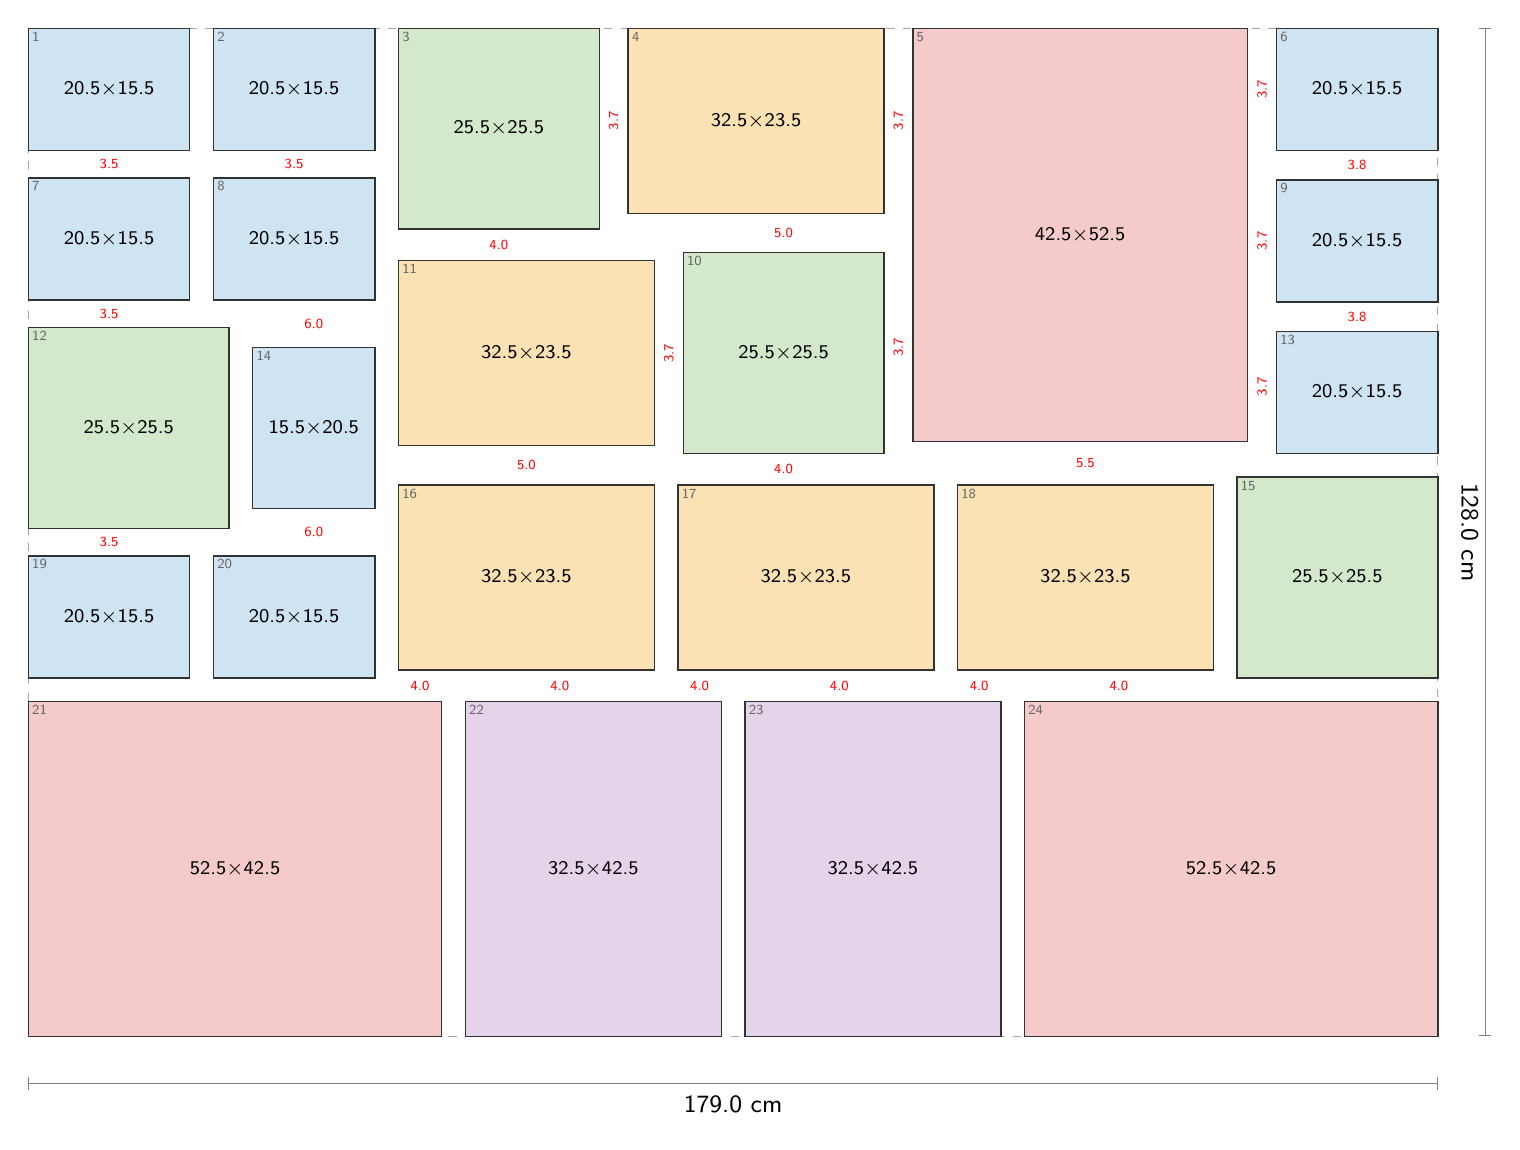
\begin{tikzpicture}[x=1mm, y=-1mm]
\draw[gray!70, dashed, line width=0.4pt] (0,0) rectangle (179.00,128.00);
\filldraw[fill=ft0, draw=black!80, line width=0.5pt] (0.00,0.00) rectangle (20.50,15.50);
\node[align=center, inner sep=0pt] at (10.25,7.75) {\scriptsize 20.5$\times$15.5};
\node[anchor=north west, inner sep=1.2pt, font=\tiny, text=black!60] at (0.00,0.00) {1};
\filldraw[fill=ft0, draw=black!80, line width=0.5pt] (23.50,0.00) rectangle (44.00,15.50);
\node[align=center, inner sep=0pt] at (33.75,7.75) {\scriptsize 20.5$\times$15.5};
\node[anchor=north west, inner sep=1.2pt, font=\tiny, text=black!60] at (23.50,0.00) {2};
\filldraw[fill=ft2, draw=black!80, line width=0.5pt] (47.00,0.00) rectangle (72.50,25.50);
\node[align=center, inner sep=0pt] at (59.75,12.75) {\scriptsize 25.5$\times$25.5};
\node[anchor=north west, inner sep=1.2pt, font=\tiny, text=black!60] at (47.00,0.00) {3};
\filldraw[fill=ft1, draw=black!80, line width=0.5pt] (76.17,0.00) rectangle (108.67,23.50);
\node[align=center, inner sep=0pt] at (92.42,11.75) {\scriptsize 32.5$\times$23.5};
\node[anchor=north west, inner sep=1.2pt, font=\tiny, text=black!60] at (76.17,0.00) {4};
\filldraw[fill=ft4, draw=black!80, line width=0.5pt] (112.33,0.00) rectangle (154.83,52.50);
\node[align=center, inner sep=0pt] at (133.58,26.25) {\scriptsize 42.5$\times$52.5};
\node[anchor=north west, inner sep=1.2pt, font=\tiny, text=black!60] at (112.33,0.00) {5};
\filldraw[fill=ft0, draw=black!80, line width=0.5pt] (158.50,0.00) rectangle (179.00,15.50);
\node[align=center, inner sep=0pt] at (168.75,7.75) {\scriptsize 20.5$\times$15.5};
\node[anchor=north west, inner sep=1.2pt, font=\tiny, text=black!60] at (158.50,0.00) {6};
\filldraw[fill=ft0, draw=black!80, line width=0.5pt] (0.00,19.00) rectangle (20.50,34.50);
\node[align=center, inner sep=0pt] at (10.25,26.75) {\scriptsize 20.5$\times$15.5};
\node[anchor=north west, inner sep=1.2pt, font=\tiny, text=black!60] at (0.00,19.00) {7};
\filldraw[fill=ft0, draw=black!80, line width=0.5pt] (23.50,19.00) rectangle (44.00,34.50);
\node[align=center, inner sep=0pt] at (33.75,26.75) {\scriptsize 20.5$\times$15.5};
\node[anchor=north west, inner sep=1.2pt, font=\tiny, text=black!60] at (23.50,19.00) {8};
\filldraw[fill=ft0, draw=black!80, line width=0.5pt] (158.50,19.25) rectangle (179.00,34.75);
\node[align=center, inner sep=0pt] at (168.75,27.00) {\scriptsize 20.5$\times$15.5};
\node[anchor=north west, inner sep=1.2pt, font=\tiny, text=black!60] at (158.50,19.25) {9};
\filldraw[fill=ft2, draw=black!80, line width=0.5pt] (83.17,28.50) rectangle (108.67,54.00);
\node[align=center, inner sep=0pt] at (95.92,41.25) {\scriptsize 25.5$\times$25.5};
\node[anchor=north west, inner sep=1.2pt, font=\tiny, text=black!60] at (83.17,28.50) {10};
\filldraw[fill=ft1, draw=black!80, line width=0.5pt] (47.00,29.50) rectangle (79.50,53.00);
\node[align=center, inner sep=0pt] at (63.25,41.25) {\scriptsize 32.5$\times$23.5};
\node[anchor=north west, inner sep=1.2pt, font=\tiny, text=black!60] at (47.00,29.50) {11};
\filldraw[fill=ft2, draw=black!80, line width=0.5pt] (0.00,38.00) rectangle (25.50,63.50);
\node[align=center, inner sep=0pt] at (12.75,50.75) {\scriptsize 25.5$\times$25.5};
\node[anchor=north west, inner sep=1.2pt, font=\tiny, text=black!60] at (0.00,38.00) {12};
\filldraw[fill=ft0, draw=black!80, line width=0.5pt] (158.50,38.50) rectangle (179.00,54.00);
\node[align=center, inner sep=0pt] at (168.75,46.25) {\scriptsize 20.5$\times$15.5};
\node[anchor=north west, inner sep=1.2pt, font=\tiny, text=black!60] at (158.50,38.50) {13};
\filldraw[fill=ft0, draw=black!80, line width=0.5pt] (28.50,40.50) rectangle (44.00,61.00);
\node[align=center, inner sep=0pt] at (36.25,50.75) {\scriptsize 15.5$\times$20.5};
\node[anchor=north west, inner sep=1.2pt, font=\tiny, text=black!60] at (28.50,40.50) {14};
\filldraw[fill=ft2, draw=black!80, line width=0.5pt] (153.50,57.00) rectangle (179.00,82.50);
\node[align=center, inner sep=0pt] at (166.25,69.75) {\scriptsize 25.5$\times$25.5};
\node[anchor=north west, inner sep=1.2pt, font=\tiny, text=black!60] at (153.50,57.00) {15};
\filldraw[fill=ft1, draw=black!80, line width=0.5pt] (47.00,58.00) rectangle (79.50,81.50);
\node[align=center, inner sep=0pt] at (63.25,69.75) {\scriptsize 32.5$\times$23.5};
\node[anchor=north west, inner sep=1.2pt, font=\tiny, text=black!60] at (47.00,58.00) {16};
\filldraw[fill=ft1, draw=black!80, line width=0.5pt] (82.50,58.00) rectangle (115.00,81.50);
\node[align=center, inner sep=0pt] at (98.75,69.75) {\scriptsize 32.5$\times$23.5};
\node[anchor=north west, inner sep=1.2pt, font=\tiny, text=black!60] at (82.50,58.00) {17};
\filldraw[fill=ft1, draw=black!80, line width=0.5pt] (118.00,58.00) rectangle (150.50,81.50);
\node[align=center, inner sep=0pt] at (134.25,69.75) {\scriptsize 32.5$\times$23.5};
\node[anchor=north west, inner sep=1.2pt, font=\tiny, text=black!60] at (118.00,58.00) {18};
\filldraw[fill=ft0, draw=black!80, line width=0.5pt] (0.00,67.00) rectangle (20.50,82.50);
\node[align=center, inner sep=0pt] at (10.25,74.75) {\scriptsize 20.5$\times$15.5};
\node[anchor=north west, inner sep=1.2pt, font=\tiny, text=black!60] at (0.00,67.00) {19};
\filldraw[fill=ft0, draw=black!80, line width=0.5pt] (23.50,67.00) rectangle (44.00,82.50);
\node[align=center, inner sep=0pt] at (33.75,74.75) {\scriptsize 20.5$\times$15.5};
\node[anchor=north west, inner sep=1.2pt, font=\tiny, text=black!60] at (23.50,67.00) {20};
\filldraw[fill=ft4, draw=black!80, line width=0.5pt] (0.00,85.50) rectangle (52.50,128.00);
\node[align=center, inner sep=0pt] at (26.25,106.75) {\scriptsize 52.5$\times$42.5};
\node[anchor=north west, inner sep=1.2pt, font=\tiny, text=black!60] at (0.00,85.50) {21};
\filldraw[fill=ft3, draw=black!80, line width=0.5pt] (55.50,85.50) rectangle (88.00,128.00);
\node[align=center, inner sep=0pt] at (71.75,106.75) {\scriptsize 32.5$\times$42.5};
\node[anchor=north west, inner sep=1.2pt, font=\tiny, text=black!60] at (55.50,85.50) {22};
\filldraw[fill=ft3, draw=black!80, line width=0.5pt] (91.00,85.50) rectangle (123.50,128.00);
\node[align=center, inner sep=0pt] at (107.25,106.75) {\scriptsize 32.5$\times$42.5};
\node[anchor=north west, inner sep=1.2pt, font=\tiny, text=black!60] at (91.00,85.50) {23};
\filldraw[fill=ft4, draw=black!80, line width=0.5pt] (126.50,85.50) rectangle (179.00,128.00);
\node[align=center, inner sep=0pt] at (152.75,106.75) {\scriptsize 52.5$\times$42.5};
\node[anchor=north west, inner sep=1.2pt, font=\tiny, text=black!60] at (126.50,85.50) {24};
\node[font=\tiny, text=red, fill=white, inner sep=0.3pt] at (10.25,17.25) {3.5};
\node[font=\tiny, text=red, fill=white, inner sep=0.3pt] at (33.75,17.25) {3.5};
\node[font=\tiny, text=red, fill=white, inner sep=0.3pt, rotate=90] at (74.33,11.75) {3.7};
\node[font=\tiny, text=red, fill=white, inner sep=0.3pt] at (59.75,27.50) {4.0};
\node[font=\tiny, text=red, fill=white, inner sep=0.3pt, rotate=90] at (110.50,11.75) {3.7};
\node[font=\tiny, text=red, fill=white, inner sep=0.3pt] at (95.92,26.00) {5.0};
\node[font=\tiny, text=red, fill=white, inner sep=0.3pt, rotate=90] at (156.67,7.75) {3.7};
\node[font=\tiny, text=red, fill=white, inner sep=0.3pt, rotate=90] at (156.67,27.00) {3.7};
\node[font=\tiny, text=red, fill=white, inner sep=0.3pt, rotate=90] at (156.67,45.50) {3.7};
\node[font=\tiny, text=red, fill=white, inner sep=0.3pt] at (134.25,55.25) {5.5};
\node[font=\tiny, text=red, fill=white, inner sep=0.3pt] at (168.75,17.38) {3.8};
\node[font=\tiny, text=red, fill=white, inner sep=0.3pt] at (10.25,36.25) {3.5};
\node[font=\tiny, text=red, fill=white, inner sep=0.3pt] at (36.25,37.50) {6.0};
\node[font=\tiny, text=red, fill=white, inner sep=0.3pt] at (168.75,36.62) {3.8};
\node[font=\tiny, text=red, fill=white, inner sep=0.3pt, rotate=90] at (110.50,40.50) {3.7};
\node[font=\tiny, text=red, fill=white, inner sep=0.3pt] at (95.92,56.00) {4.0};
\node[font=\tiny, text=red, fill=white, inner sep=0.3pt, rotate=90] at (81.33,41.25) {3.7};
\node[font=\tiny, text=red, fill=white, inner sep=0.3pt] at (63.25,55.50) {5.0};
\node[font=\tiny, text=red, fill=white, inner sep=0.3pt] at (10.25,65.25) {3.5};
\node[font=\tiny, text=red, fill=white, inner sep=0.3pt] at (36.25,64.00) {6.0};
\node[font=\tiny, text=red, fill=white, inner sep=0.3pt] at (49.75,83.50) {4.0};
\node[font=\tiny, text=red, fill=white, inner sep=0.3pt] at (67.50,83.50) {4.0};
\node[font=\tiny, text=red, fill=white, inner sep=0.3pt] at (85.25,83.50) {4.0};
\node[font=\tiny, text=red, fill=white, inner sep=0.3pt] at (103.00,83.50) {4.0};
\node[font=\tiny, text=red, fill=white, inner sep=0.3pt] at (120.75,83.50) {4.0};
\node[font=\tiny, text=red, fill=white, inner sep=0.3pt] at (138.50,83.50) {4.0};
\draw[Bar-Bar, gray] (0,134.00) -- (179.00,134.00) node[midway, below=1pt, font=\small, text=black] {179.0 cm};
\draw[Bar-Bar, gray] (185.00,0) -- (185.00,128.00) node[midway, right=1pt, font=\small, text=black, rotate=-90, anchor=north] {128.0 cm};
\end{tikzpicture}\\[4pt]
{\scriptsize Scale 1:10 (1 mm = 1 cm). Red numbers mark gaps that deviate from the nominal gap by more than 0.25 cm. Small grey numbers index the coordinate table.}
\end{minipage}\hfill
\begin{minipage}[t]{0.25\textwidth}\vspace{0pt}
\small
\begin{tabular}{@{}l l@{}}
\toprule
Outer size & 179.0 $\times$ 128.0 cm \\
Nominal gap & 3 cm \\
Actual gaps & 3.0 -- 6.0 cm \\
Max.\ deviation & 3.0 cm \\
Mean deviation & 0.64 cm \\
Border notches & none \\
Corners filled & 4 / 4 \\
Frames used & 24 of 28 \\
\bottomrule
\end{tabular}

\vspace{8pt}
\scriptsize
\begin{tabular}{@{}c l l r r@{}}
\toprule
 & outer w $\times$ h (cm) & & used & have \\
\midrule
\tikz[baseline=-0.6ex]\fill[ft0,draw=black!60] (0,0) rectangle (1.2ex,1.2ex); & 20.5$\times$15.5 & L & 9 & 9 \\
\tikz[baseline=-0.6ex]\fill[ft0,draw=black!60] (0,0) rectangle (1.2ex,1.2ex); & 15.5$\times$20.5 & P & 1 & 2 \\
\tikz[baseline=-0.6ex]\fill[ft3,draw=black!60] (0,0) rectangle (1.2ex,1.2ex); & 32.5$\times$42.5 & P & 2 & 2 \\
\tikz[baseline=-0.6ex]\fill[ft3,draw=black!60] (0,0) rectangle (1.2ex,1.2ex); & 42.5$\times$32.5 & L & 0 & 1 \\
\tikz[baseline=-0.6ex]\fill[ft1,draw=black!60] (0,0) rectangle (1.2ex,1.2ex); & 32.5$\times$23.5 & L & 5 & 5 \\
\tikz[baseline=-0.6ex]\fill[ft1,draw=black!60] (0,0) rectangle (1.2ex,1.2ex); & 23.5$\times$32.5 & P & 0 & 1 \\
\tikz[baseline=-0.6ex]\fill[ft2,draw=black!60] (0,0) rectangle (1.2ex,1.2ex); & 25.5$\times$25.5 &  & 4 & 5 \\
\tikz[baseline=-0.6ex]\fill[ft4,draw=black!60] (0,0) rectangle (1.2ex,1.2ex); & 42.5$\times$52.5 & P & 1 & 1 \\
\tikz[baseline=-0.6ex]\fill[ft4,draw=black!60] (0,0) rectangle (1.2ex,1.2ex); & 52.5$\times$42.5 & L & 2 & 2 \\
\bottomrule
\end{tabular}

\vspace{8pt}
{\bfseries Positions} (top-left corner, cm)\\[2pt]
\tiny
\begin{tabular}{@{}r l r r@{}}
\toprule
\# & frame w $\times$ h & x & y \\
\midrule
1 & 20.5 $\times$ 15.5 & 0.0 & 0.0 \\
2 & 20.5 $\times$ 15.5 & 23.5 & 0.0 \\
3 & 25.5 $\times$ 25.5 & 47.0 & 0.0 \\
4 & 32.5 $\times$ 23.5 & 76.2 & 0.0 \\
5 & 42.5 $\times$ 52.5 & 112.3 & 0.0 \\
6 & 20.5 $\times$ 15.5 & 158.5 & 0.0 \\
7 & 20.5 $\times$ 15.5 & 0.0 & 19.0 \\
8 & 20.5 $\times$ 15.5 & 23.5 & 19.0 \\
9 & 20.5 $\times$ 15.5 & 158.5 & 19.2 \\
10 & 25.5 $\times$ 25.5 & 83.2 & 28.5 \\
11 & 32.5 $\times$ 23.5 & 47.0 & 29.5 \\
12 & 25.5 $\times$ 25.5 & 0.0 & 38.0 \\
13 & 20.5 $\times$ 15.5 & 158.5 & 38.5 \\
14 & 15.5 $\times$ 20.5 & 28.5 & 40.5 \\
15 & 25.5 $\times$ 25.5 & 153.5 & 57.0 \\
16 & 32.5 $\times$ 23.5 & 47.0 & 58.0 \\
17 & 32.5 $\times$ 23.5 & 82.5 & 58.0 \\
18 & 32.5 $\times$ 23.5 & 118.0 & 58.0 \\
19 & 20.5 $\times$ 15.5 & 0.0 & 67.0 \\
20 & 20.5 $\times$ 15.5 & 23.5 & 67.0 \\
21 & 52.5 $\times$ 42.5 & 0.0 & 85.5 \\
22 & 32.5 $\times$ 42.5 & 55.5 & 85.5 \\
23 & 32.5 $\times$ 42.5 & 91.0 & 85.5 \\
24 & 52.5 $\times$ 42.5 & 126.5 & 85.5 \\
\bottomrule
\end{tabular}
\end{minipage}
\clearpage

\begin{minipage}[t]{0.74\textwidth}\vspace{0pt}
{\LARGE\bfseries Layout 6}\hspace{1.5em}{\large 189.0 $\times$ 109.0 cm \quad gap 3 cm \quad 24 frames}\\[8pt]
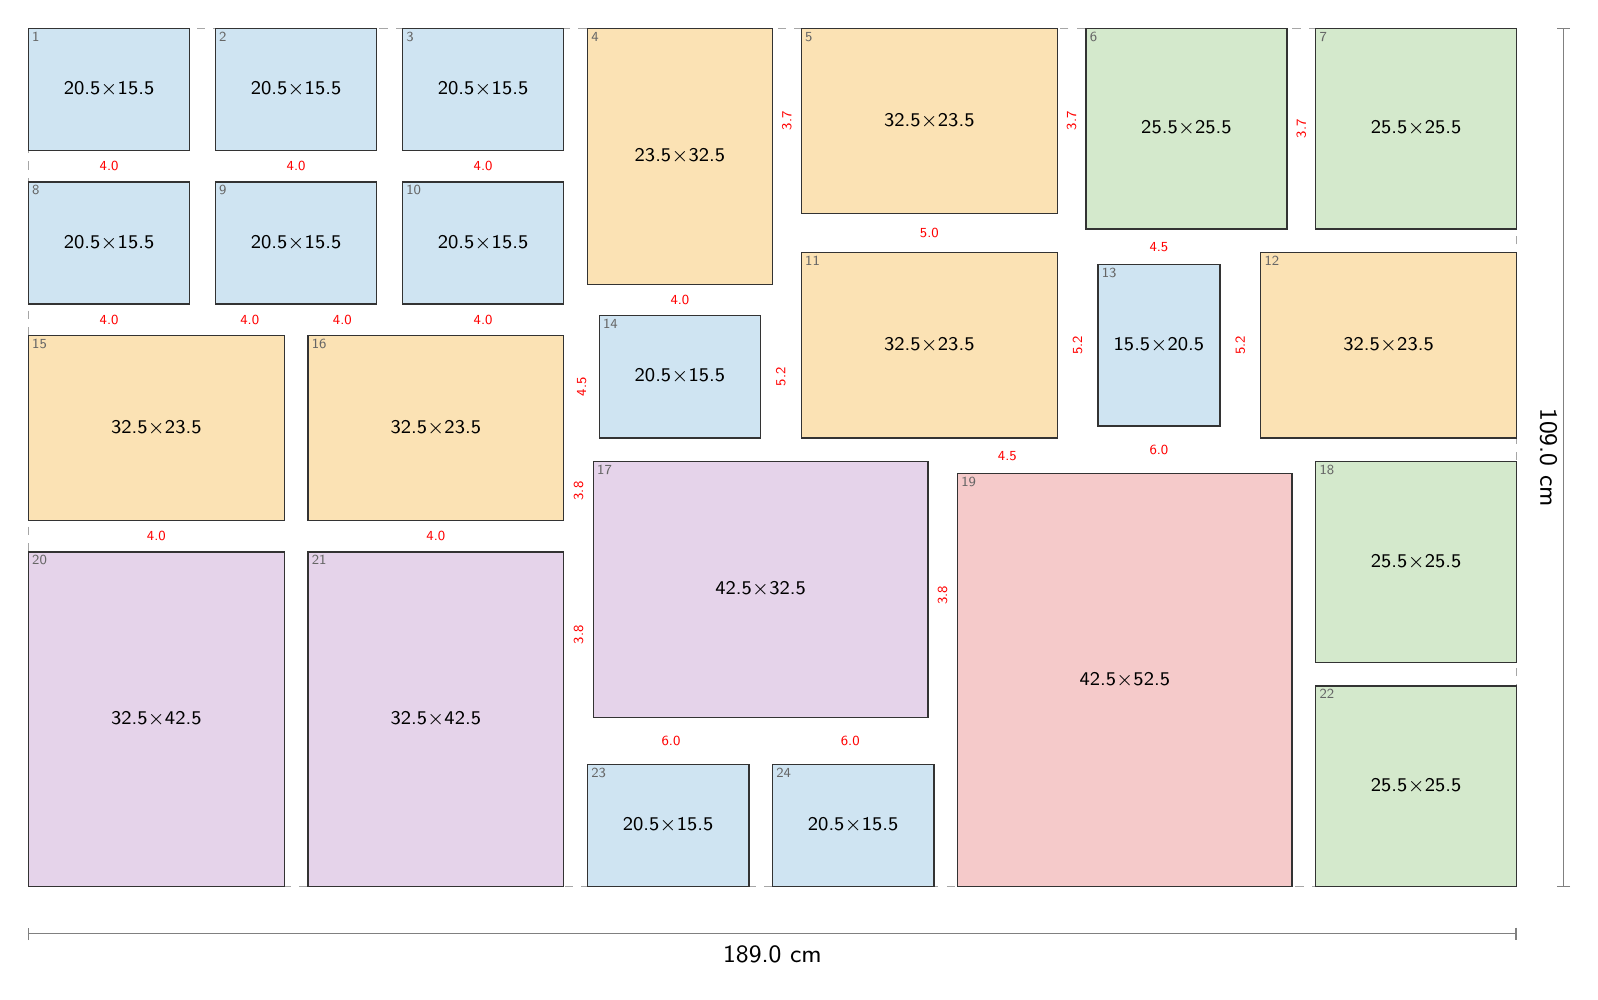
\begin{tikzpicture}[x=1mm, y=-1mm]
\draw[gray!70, dashed, line width=0.4pt] (0,0) rectangle (189.00,109.00);
\filldraw[fill=ft0, draw=black!80, line width=0.5pt] (0.00,0.00) rectangle (20.50,15.50);
\node[align=center, inner sep=0pt] at (10.25,7.75) {\scriptsize 20.5$\times$15.5};
\node[anchor=north west, inner sep=1.2pt, font=\tiny, text=black!60] at (0.00,0.00) {1};
\filldraw[fill=ft0, draw=black!80, line width=0.5pt] (23.75,0.00) rectangle (44.25,15.50);
\node[align=center, inner sep=0pt] at (34.00,7.75) {\scriptsize 20.5$\times$15.5};
\node[anchor=north west, inner sep=1.2pt, font=\tiny, text=black!60] at (23.75,0.00) {2};
\filldraw[fill=ft0, draw=black!80, line width=0.5pt] (47.50,0.00) rectangle (68.00,15.50);
\node[align=center, inner sep=0pt] at (57.75,7.75) {\scriptsize 20.5$\times$15.5};
\node[anchor=north west, inner sep=1.2pt, font=\tiny, text=black!60] at (47.50,0.00) {3};
\filldraw[fill=ft1, draw=black!80, line width=0.5pt] (71.00,0.00) rectangle (94.50,32.50);
\node[align=center, inner sep=0pt] at (82.75,16.25) {\scriptsize 23.5$\times$32.5};
\node[anchor=north west, inner sep=1.2pt, font=\tiny, text=black!60] at (71.00,0.00) {4};
\filldraw[fill=ft1, draw=black!80, line width=0.5pt] (98.17,0.00) rectangle (130.67,23.50);
\node[align=center, inner sep=0pt] at (114.42,11.75) {\scriptsize 32.5$\times$23.5};
\node[anchor=north west, inner sep=1.2pt, font=\tiny, text=black!60] at (98.17,0.00) {5};
\filldraw[fill=ft2, draw=black!80, line width=0.5pt] (134.33,0.00) rectangle (159.83,25.50);
\node[align=center, inner sep=0pt] at (147.08,12.75) {\scriptsize 25.5$\times$25.5};
\node[anchor=north west, inner sep=1.2pt, font=\tiny, text=black!60] at (134.33,0.00) {6};
\filldraw[fill=ft2, draw=black!80, line width=0.5pt] (163.50,0.00) rectangle (189.00,25.50);
\node[align=center, inner sep=0pt] at (176.25,12.75) {\scriptsize 25.5$\times$25.5};
\node[anchor=north west, inner sep=1.2pt, font=\tiny, text=black!60] at (163.50,0.00) {7};
\filldraw[fill=ft0, draw=black!80, line width=0.5pt] (0.00,19.50) rectangle (20.50,35.00);
\node[align=center, inner sep=0pt] at (10.25,27.25) {\scriptsize 20.5$\times$15.5};
\node[anchor=north west, inner sep=1.2pt, font=\tiny, text=black!60] at (0.00,19.50) {8};
\filldraw[fill=ft0, draw=black!80, line width=0.5pt] (23.75,19.50) rectangle (44.25,35.00);
\node[align=center, inner sep=0pt] at (34.00,27.25) {\scriptsize 20.5$\times$15.5};
\node[anchor=north west, inner sep=1.2pt, font=\tiny, text=black!60] at (23.75,19.50) {9};
\filldraw[fill=ft0, draw=black!80, line width=0.5pt] (47.50,19.50) rectangle (68.00,35.00);
\node[align=center, inner sep=0pt] at (57.75,27.25) {\scriptsize 20.5$\times$15.5};
\node[anchor=north west, inner sep=1.2pt, font=\tiny, text=black!60] at (47.50,19.50) {10};
\filldraw[fill=ft1, draw=black!80, line width=0.5pt] (98.17,28.50) rectangle (130.67,52.00);
\node[align=center, inner sep=0pt] at (114.42,40.25) {\scriptsize 32.5$\times$23.5};
\node[anchor=north west, inner sep=1.2pt, font=\tiny, text=black!60] at (98.17,28.50) {11};
\filldraw[fill=ft1, draw=black!80, line width=0.5pt] (156.50,28.50) rectangle (189.00,52.00);
\node[align=center, inner sep=0pt] at (172.75,40.25) {\scriptsize 32.5$\times$23.5};
\node[anchor=north west, inner sep=1.2pt, font=\tiny, text=black!60] at (156.50,28.50) {12};
\filldraw[fill=ft0, draw=black!80, line width=0.5pt] (135.83,30.00) rectangle (151.33,50.50);
\node[align=center, inner sep=0pt] at (143.58,40.25) {\scriptsize 15.5$\times$20.5};
\node[anchor=north west, inner sep=1.2pt, font=\tiny, text=black!60] at (135.83,30.00) {13};
\filldraw[fill=ft0, draw=black!80, line width=0.5pt] (72.50,36.50) rectangle (93.00,52.00);
\node[align=center, inner sep=0pt] at (82.75,44.25) {\scriptsize 20.5$\times$15.5};
\node[anchor=north west, inner sep=1.2pt, font=\tiny, text=black!60] at (72.50,36.50) {14};
\filldraw[fill=ft1, draw=black!80, line width=0.5pt] (0.00,39.00) rectangle (32.50,62.50);
\node[align=center, inner sep=0pt] at (16.25,50.75) {\scriptsize 32.5$\times$23.5};
\node[anchor=north west, inner sep=1.2pt, font=\tiny, text=black!60] at (0.00,39.00) {15};
\filldraw[fill=ft1, draw=black!80, line width=0.5pt] (35.50,39.00) rectangle (68.00,62.50);
\node[align=center, inner sep=0pt] at (51.75,50.75) {\scriptsize 32.5$\times$23.5};
\node[anchor=north west, inner sep=1.2pt, font=\tiny, text=black!60] at (35.50,39.00) {16};
\filldraw[fill=ft3, draw=black!80, line width=0.5pt] (71.75,55.00) rectangle (114.25,87.50);
\node[align=center, inner sep=0pt] at (93.00,71.25) {\scriptsize 42.5$\times$32.5};
\node[anchor=north west, inner sep=1.2pt, font=\tiny, text=black!60] at (71.75,55.00) {17};
\filldraw[fill=ft2, draw=black!80, line width=0.5pt] (163.50,55.00) rectangle (189.00,80.50);
\node[align=center, inner sep=0pt] at (176.25,67.75) {\scriptsize 25.5$\times$25.5};
\node[anchor=north west, inner sep=1.2pt, font=\tiny, text=black!60] at (163.50,55.00) {18};
\filldraw[fill=ft4, draw=black!80, line width=0.5pt] (118.00,56.50) rectangle (160.50,109.00);
\node[align=center, inner sep=0pt] at (139.25,82.75) {\scriptsize 42.5$\times$52.5};
\node[anchor=north west, inner sep=1.2pt, font=\tiny, text=black!60] at (118.00,56.50) {19};
\filldraw[fill=ft3, draw=black!80, line width=0.5pt] (0.00,66.50) rectangle (32.50,109.00);
\node[align=center, inner sep=0pt] at (16.25,87.75) {\scriptsize 32.5$\times$42.5};
\node[anchor=north west, inner sep=1.2pt, font=\tiny, text=black!60] at (0.00,66.50) {20};
\filldraw[fill=ft3, draw=black!80, line width=0.5pt] (35.50,66.50) rectangle (68.00,109.00);
\node[align=center, inner sep=0pt] at (51.75,87.75) {\scriptsize 32.5$\times$42.5};
\node[anchor=north west, inner sep=1.2pt, font=\tiny, text=black!60] at (35.50,66.50) {21};
\filldraw[fill=ft2, draw=black!80, line width=0.5pt] (163.50,83.50) rectangle (189.00,109.00);
\node[align=center, inner sep=0pt] at (176.25,96.25) {\scriptsize 25.5$\times$25.5};
\node[anchor=north west, inner sep=1.2pt, font=\tiny, text=black!60] at (163.50,83.50) {22};
\filldraw[fill=ft0, draw=black!80, line width=0.5pt] (71.00,93.50) rectangle (91.50,109.00);
\node[align=center, inner sep=0pt] at (81.25,101.25) {\scriptsize 20.5$\times$15.5};
\node[anchor=north west, inner sep=1.2pt, font=\tiny, text=black!60] at (71.00,93.50) {23};
\filldraw[fill=ft0, draw=black!80, line width=0.5pt] (94.50,93.50) rectangle (115.00,109.00);
\node[align=center, inner sep=0pt] at (104.75,101.25) {\scriptsize 20.5$\times$15.5};
\node[anchor=north west, inner sep=1.2pt, font=\tiny, text=black!60] at (94.50,93.50) {24};
\node[font=\tiny, text=red, fill=white, inner sep=0.3pt] at (10.25,17.50) {4.0};
\node[font=\tiny, text=red, fill=white, inner sep=0.3pt] at (34.00,17.50) {4.0};
\node[font=\tiny, text=red, fill=white, inner sep=0.3pt] at (57.75,17.50) {4.0};
\node[font=\tiny, text=red, fill=white, inner sep=0.3pt, rotate=90] at (96.33,11.75) {3.7};
\node[font=\tiny, text=red, fill=white, inner sep=0.3pt] at (82.75,34.50) {4.0};
\node[font=\tiny, text=red, fill=white, inner sep=0.3pt, rotate=90] at (132.50,11.75) {3.7};
\node[font=\tiny, text=red, fill=white, inner sep=0.3pt] at (114.42,26.00) {5.0};
\node[font=\tiny, text=red, fill=white, inner sep=0.3pt, rotate=90] at (161.67,12.75) {3.7};
\node[font=\tiny, text=red, fill=white, inner sep=0.3pt] at (143.58,27.75) {4.5};
\node[font=\tiny, text=red, fill=white, inner sep=0.3pt] at (10.25,37.00) {4.0};
\node[font=\tiny, text=red, fill=white, inner sep=0.3pt] at (28.12,37.00) {4.0};
\node[font=\tiny, text=red, fill=white, inner sep=0.3pt] at (39.88,37.00) {4.0};
\node[font=\tiny, text=red, fill=white, inner sep=0.3pt] at (57.75,37.00) {4.0};
\node[font=\tiny, text=red, fill=white, inner sep=0.3pt, rotate=90] at (133.25,40.25) {5.2};
\node[font=\tiny, text=red, fill=white, inner sep=0.3pt] at (124.33,54.25) {4.5};
\node[font=\tiny, text=red, fill=white, inner sep=0.3pt, rotate=90] at (153.92,40.25) {5.2};
\node[font=\tiny, text=red, fill=white, inner sep=0.3pt] at (143.58,53.50) {6.0};
\node[font=\tiny, text=red, fill=white, inner sep=0.3pt, rotate=90] at (95.58,44.25) {5.2};
\node[font=\tiny, text=red, fill=white, inner sep=0.3pt] at (16.25,64.50) {4.0};
\node[font=\tiny, text=red, fill=white, inner sep=0.3pt, rotate=90] at (70.25,45.50) {4.5};
\node[font=\tiny, text=red, fill=white, inner sep=0.3pt, rotate=90] at (69.88,58.75) {3.8};
\node[font=\tiny, text=red, fill=white, inner sep=0.3pt] at (51.75,64.50) {4.0};
\node[font=\tiny, text=red, fill=white, inner sep=0.3pt, rotate=90] at (116.12,72.00) {3.8};
\node[font=\tiny, text=red, fill=white, inner sep=0.3pt] at (81.62,90.50) {6.0};
\node[font=\tiny, text=red, fill=white, inner sep=0.3pt] at (104.38,90.50) {6.0};
\node[font=\tiny, text=red, fill=white, inner sep=0.3pt, rotate=90] at (69.88,77.00) {3.8};
\draw[Bar-Bar, gray] (0,115.00) -- (189.00,115.00) node[midway, below=1pt, font=\small, text=black] {189.0 cm};
\draw[Bar-Bar, gray] (195.00,0) -- (195.00,109.00) node[midway, right=1pt, font=\small, text=black, rotate=-90, anchor=north] {109.0 cm};
\end{tikzpicture}\\[4pt]
{\scriptsize Scale 1:10 (1 mm = 1 cm). Red numbers mark gaps that deviate from the nominal gap by more than 0.25 cm. Small grey numbers index the coordinate table.}
\end{minipage}\hfill
\begin{minipage}[t]{0.25\textwidth}\vspace{0pt}
\small
\begin{tabular}{@{}l l@{}}
\toprule
Outer size & 189.0 $\times$ 109.0 cm \\
Nominal gap & 3 cm \\
Actual gaps & 3.0 -- 6.0 cm \\
Max.\ deviation & 3.0 cm \\
Mean deviation & 0.85 cm \\
Border notches & none \\
Corners filled & 4 / 4 \\
Frames used & 24 of 28 \\
\bottomrule
\end{tabular}

\vspace{8pt}
\scriptsize
\begin{tabular}{@{}c l l r r@{}}
\toprule
 & outer w $\times$ h (cm) & & used & have \\
\midrule
\tikz[baseline=-0.6ex]\fill[ft0,draw=black!60] (0,0) rectangle (1.2ex,1.2ex); & 20.5$\times$15.5 & L & 9 & 9 \\
\tikz[baseline=-0.6ex]\fill[ft0,draw=black!60] (0,0) rectangle (1.2ex,1.2ex); & 15.5$\times$20.5 & P & 1 & 2 \\
\tikz[baseline=-0.6ex]\fill[ft3,draw=black!60] (0,0) rectangle (1.2ex,1.2ex); & 32.5$\times$42.5 & P & 2 & 2 \\
\tikz[baseline=-0.6ex]\fill[ft3,draw=black!60] (0,0) rectangle (1.2ex,1.2ex); & 42.5$\times$32.5 & L & 1 & 1 \\
\tikz[baseline=-0.6ex]\fill[ft1,draw=black!60] (0,0) rectangle (1.2ex,1.2ex); & 32.5$\times$23.5 & L & 5 & 5 \\
\tikz[baseline=-0.6ex]\fill[ft1,draw=black!60] (0,0) rectangle (1.2ex,1.2ex); & 23.5$\times$32.5 & P & 1 & 1 \\
\tikz[baseline=-0.6ex]\fill[ft2,draw=black!60] (0,0) rectangle (1.2ex,1.2ex); & 25.5$\times$25.5 &  & 4 & 5 \\
\tikz[baseline=-0.6ex]\fill[ft4,draw=black!60] (0,0) rectangle (1.2ex,1.2ex); & 42.5$\times$52.5 & P & 1 & 1 \\
\tikz[baseline=-0.6ex]\fill[ft4,draw=black!60] (0,0) rectangle (1.2ex,1.2ex); & 52.5$\times$42.5 & L & 0 & 2 \\
\bottomrule
\end{tabular}

\vspace{8pt}
{\bfseries Positions} (top-left corner, cm)\\[2pt]
\tiny
\begin{tabular}{@{}r l r r@{}}
\toprule
\# & frame w $\times$ h & x & y \\
\midrule
1 & 20.5 $\times$ 15.5 & 0.0 & 0.0 \\
2 & 20.5 $\times$ 15.5 & 23.8 & 0.0 \\
3 & 20.5 $\times$ 15.5 & 47.5 & 0.0 \\
4 & 23.5 $\times$ 32.5 & 71.0 & 0.0 \\
5 & 32.5 $\times$ 23.5 & 98.2 & 0.0 \\
6 & 25.5 $\times$ 25.5 & 134.3 & 0.0 \\
7 & 25.5 $\times$ 25.5 & 163.5 & 0.0 \\
8 & 20.5 $\times$ 15.5 & 0.0 & 19.5 \\
9 & 20.5 $\times$ 15.5 & 23.8 & 19.5 \\
10 & 20.5 $\times$ 15.5 & 47.5 & 19.5 \\
11 & 32.5 $\times$ 23.5 & 98.2 & 28.5 \\
12 & 32.5 $\times$ 23.5 & 156.5 & 28.5 \\
13 & 15.5 $\times$ 20.5 & 135.8 & 30.0 \\
14 & 20.5 $\times$ 15.5 & 72.5 & 36.5 \\
15 & 32.5 $\times$ 23.5 & 0.0 & 39.0 \\
16 & 32.5 $\times$ 23.5 & 35.5 & 39.0 \\
17 & 42.5 $\times$ 32.5 & 71.8 & 55.0 \\
18 & 25.5 $\times$ 25.5 & 163.5 & 55.0 \\
19 & 42.5 $\times$ 52.5 & 118.0 & 56.5 \\
20 & 32.5 $\times$ 42.5 & 0.0 & 66.5 \\
21 & 32.5 $\times$ 42.5 & 35.5 & 66.5 \\
22 & 25.5 $\times$ 25.5 & 163.5 & 83.5 \\
23 & 20.5 $\times$ 15.5 & 71.0 & 93.5 \\
24 & 20.5 $\times$ 15.5 & 94.5 & 93.5 \\
\bottomrule
\end{tabular}
\end{minipage}
\clearpage

\begin{minipage}[t]{0.74\textwidth}\vspace{0pt}
{\LARGE\bfseries Layout 7}\hspace{1.5em}{\large 173.5 $\times$ 118.0 cm \quad gap 3 cm \quad 23 frames}\\[8pt]
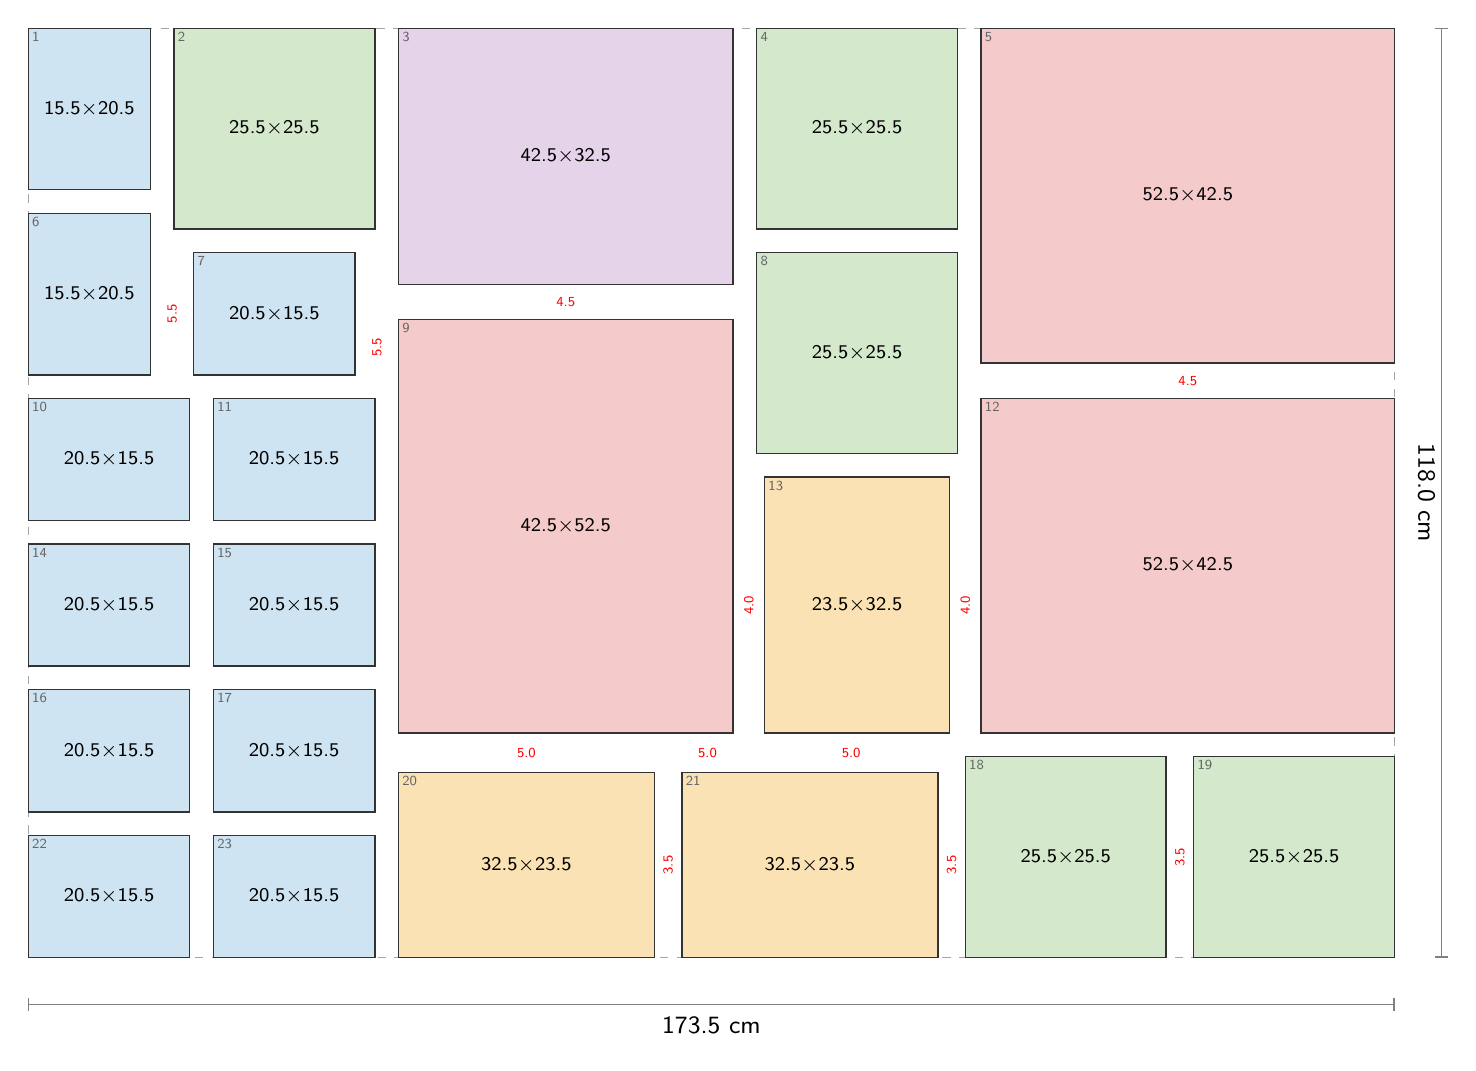
\begin{tikzpicture}[x=1mm, y=-1mm]
\draw[gray!70, dashed, line width=0.4pt] (0,0) rectangle (173.50,118.00);
\filldraw[fill=ft0, draw=black!80, line width=0.5pt] (0.00,0.00) rectangle (15.50,20.50);
\node[align=center, inner sep=0pt] at (7.75,10.25) {\scriptsize 15.5$\times$20.5};
\node[anchor=north west, inner sep=1.2pt, font=\tiny, text=black!60] at (0.00,0.00) {1};
\filldraw[fill=ft2, draw=black!80, line width=0.5pt] (18.50,0.00) rectangle (44.00,25.50);
\node[align=center, inner sep=0pt] at (31.25,12.75) {\scriptsize 25.5$\times$25.5};
\node[anchor=north west, inner sep=1.2pt, font=\tiny, text=black!60] at (18.50,0.00) {2};
\filldraw[fill=ft3, draw=black!80, line width=0.5pt] (47.00,0.00) rectangle (89.50,32.50);
\node[align=center, inner sep=0pt] at (68.25,16.25) {\scriptsize 42.5$\times$32.5};
\node[anchor=north west, inner sep=1.2pt, font=\tiny, text=black!60] at (47.00,0.00) {3};
\filldraw[fill=ft2, draw=black!80, line width=0.5pt] (92.50,0.00) rectangle (118.00,25.50);
\node[align=center, inner sep=0pt] at (105.25,12.75) {\scriptsize 25.5$\times$25.5};
\node[anchor=north west, inner sep=1.2pt, font=\tiny, text=black!60] at (92.50,0.00) {4};
\filldraw[fill=ft4, draw=black!80, line width=0.5pt] (121.00,0.00) rectangle (173.50,42.50);
\node[align=center, inner sep=0pt] at (147.25,21.25) {\scriptsize 52.5$\times$42.5};
\node[anchor=north west, inner sep=1.2pt, font=\tiny, text=black!60] at (121.00,0.00) {5};
\filldraw[fill=ft0, draw=black!80, line width=0.5pt] (0.00,23.50) rectangle (15.50,44.00);
\node[align=center, inner sep=0pt] at (7.75,33.75) {\scriptsize 15.5$\times$20.5};
\node[anchor=north west, inner sep=1.2pt, font=\tiny, text=black!60] at (0.00,23.50) {6};
\filldraw[fill=ft0, draw=black!80, line width=0.5pt] (21.00,28.50) rectangle (41.50,44.00);
\node[align=center, inner sep=0pt] at (31.25,36.25) {\scriptsize 20.5$\times$15.5};
\node[anchor=north west, inner sep=1.2pt, font=\tiny, text=black!60] at (21.00,28.50) {7};
\filldraw[fill=ft2, draw=black!80, line width=0.5pt] (92.50,28.50) rectangle (118.00,54.00);
\node[align=center, inner sep=0pt] at (105.25,41.25) {\scriptsize 25.5$\times$25.5};
\node[anchor=north west, inner sep=1.2pt, font=\tiny, text=black!60] at (92.50,28.50) {8};
\filldraw[fill=ft4, draw=black!80, line width=0.5pt] (47.00,37.00) rectangle (89.50,89.50);
\node[align=center, inner sep=0pt] at (68.25,63.25) {\scriptsize 42.5$\times$52.5};
\node[anchor=north west, inner sep=1.2pt, font=\tiny, text=black!60] at (47.00,37.00) {9};
\filldraw[fill=ft0, draw=black!80, line width=0.5pt] (0.00,47.00) rectangle (20.50,62.50);
\node[align=center, inner sep=0pt] at (10.25,54.75) {\scriptsize 20.5$\times$15.5};
\node[anchor=north west, inner sep=1.2pt, font=\tiny, text=black!60] at (0.00,47.00) {10};
\filldraw[fill=ft0, draw=black!80, line width=0.5pt] (23.50,47.00) rectangle (44.00,62.50);
\node[align=center, inner sep=0pt] at (33.75,54.75) {\scriptsize 20.5$\times$15.5};
\node[anchor=north west, inner sep=1.2pt, font=\tiny, text=black!60] at (23.50,47.00) {11};
\filldraw[fill=ft4, draw=black!80, line width=0.5pt] (121.00,47.00) rectangle (173.50,89.50);
\node[align=center, inner sep=0pt] at (147.25,68.25) {\scriptsize 52.5$\times$42.5};
\node[anchor=north west, inner sep=1.2pt, font=\tiny, text=black!60] at (121.00,47.00) {12};
\filldraw[fill=ft1, draw=black!80, line width=0.5pt] (93.50,57.00) rectangle (117.00,89.50);
\node[align=center, inner sep=0pt] at (105.25,73.25) {\scriptsize 23.5$\times$32.5};
\node[anchor=north west, inner sep=1.2pt, font=\tiny, text=black!60] at (93.50,57.00) {13};
\filldraw[fill=ft0, draw=black!80, line width=0.5pt] (0.00,65.50) rectangle (20.50,81.00);
\node[align=center, inner sep=0pt] at (10.25,73.25) {\scriptsize 20.5$\times$15.5};
\node[anchor=north west, inner sep=1.2pt, font=\tiny, text=black!60] at (0.00,65.50) {14};
\filldraw[fill=ft0, draw=black!80, line width=0.5pt] (23.50,65.50) rectangle (44.00,81.00);
\node[align=center, inner sep=0pt] at (33.75,73.25) {\scriptsize 20.5$\times$15.5};
\node[anchor=north west, inner sep=1.2pt, font=\tiny, text=black!60] at (23.50,65.50) {15};
\filldraw[fill=ft0, draw=black!80, line width=0.5pt] (0.00,84.00) rectangle (20.50,99.50);
\node[align=center, inner sep=0pt] at (10.25,91.75) {\scriptsize 20.5$\times$15.5};
\node[anchor=north west, inner sep=1.2pt, font=\tiny, text=black!60] at (0.00,84.00) {16};
\filldraw[fill=ft0, draw=black!80, line width=0.5pt] (23.50,84.00) rectangle (44.00,99.50);
\node[align=center, inner sep=0pt] at (33.75,91.75) {\scriptsize 20.5$\times$15.5};
\node[anchor=north west, inner sep=1.2pt, font=\tiny, text=black!60] at (23.50,84.00) {17};
\filldraw[fill=ft2, draw=black!80, line width=0.5pt] (119.00,92.50) rectangle (144.50,118.00);
\node[align=center, inner sep=0pt] at (131.75,105.25) {\scriptsize 25.5$\times$25.5};
\node[anchor=north west, inner sep=1.2pt, font=\tiny, text=black!60] at (119.00,92.50) {18};
\filldraw[fill=ft2, draw=black!80, line width=0.5pt] (148.00,92.50) rectangle (173.50,118.00);
\node[align=center, inner sep=0pt] at (160.75,105.25) {\scriptsize 25.5$\times$25.5};
\node[anchor=north west, inner sep=1.2pt, font=\tiny, text=black!60] at (148.00,92.50) {19};
\filldraw[fill=ft1, draw=black!80, line width=0.5pt] (47.00,94.50) rectangle (79.50,118.00);
\node[align=center, inner sep=0pt] at (63.25,106.25) {\scriptsize 32.5$\times$23.5};
\node[anchor=north west, inner sep=1.2pt, font=\tiny, text=black!60] at (47.00,94.50) {20};
\filldraw[fill=ft1, draw=black!80, line width=0.5pt] (83.00,94.50) rectangle (115.50,118.00);
\node[align=center, inner sep=0pt] at (99.25,106.25) {\scriptsize 32.5$\times$23.5};
\node[anchor=north west, inner sep=1.2pt, font=\tiny, text=black!60] at (83.00,94.50) {21};
\filldraw[fill=ft0, draw=black!80, line width=0.5pt] (0.00,102.50) rectangle (20.50,118.00);
\node[align=center, inner sep=0pt] at (10.25,110.25) {\scriptsize 20.5$\times$15.5};
\node[anchor=north west, inner sep=1.2pt, font=\tiny, text=black!60] at (0.00,102.50) {22};
\filldraw[fill=ft0, draw=black!80, line width=0.5pt] (23.50,102.50) rectangle (44.00,118.00);
\node[align=center, inner sep=0pt] at (33.75,110.25) {\scriptsize 20.5$\times$15.5};
\node[anchor=north west, inner sep=1.2pt, font=\tiny, text=black!60] at (23.50,102.50) {23};
\node[font=\tiny, text=red, fill=white, inner sep=0.3pt] at (68.25,34.75) {4.5};
\node[font=\tiny, text=red, fill=white, inner sep=0.3pt] at (147.25,44.75) {4.5};
\node[font=\tiny, text=red, fill=white, inner sep=0.3pt, rotate=90] at (18.25,36.25) {5.5};
\node[font=\tiny, text=red, fill=white, inner sep=0.3pt, rotate=90] at (44.25,40.50) {5.5};
\node[font=\tiny, text=red, fill=white, inner sep=0.3pt, rotate=90] at (91.50,73.25) {4.0};
\node[font=\tiny, text=red, fill=white, inner sep=0.3pt] at (63.25,92.00) {5.0};
\node[font=\tiny, text=red, fill=white, inner sep=0.3pt] at (86.25,92.00) {5.0};
\node[font=\tiny, text=red, fill=white, inner sep=0.3pt, rotate=90] at (119.00,73.25) {4.0};
\node[font=\tiny, text=red, fill=white, inner sep=0.3pt] at (104.50,92.00) {5.0};
\node[font=\tiny, text=red, fill=white, inner sep=0.3pt, rotate=90] at (146.25,105.25) {3.5};
\node[font=\tiny, text=red, fill=white, inner sep=0.3pt, rotate=90] at (81.25,106.25) {3.5};
\node[font=\tiny, text=red, fill=white, inner sep=0.3pt, rotate=90] at (117.25,106.25) {3.5};
\draw[Bar-Bar, gray] (0,124.00) -- (173.50,124.00) node[midway, below=1pt, font=\small, text=black] {173.5 cm};
\draw[Bar-Bar, gray] (179.50,0) -- (179.50,118.00) node[midway, right=1pt, font=\small, text=black, rotate=-90, anchor=north] {118.0 cm};
\end{tikzpicture}\\[4pt]
{\scriptsize Scale 1:10 (1 mm = 1 cm). Red numbers mark gaps that deviate from the nominal gap by more than 0.25 cm. Small grey numbers index the coordinate table.}
\end{minipage}\hfill
\begin{minipage}[t]{0.25\textwidth}\vspace{0pt}
\small
\begin{tabular}{@{}l l@{}}
\toprule
Outer size & 173.5 $\times$ 118.0 cm \\
Nominal gap & 3 cm \\
Actual gaps & 3.0 -- 5.5 cm \\
Max.\ deviation & 2.5 cm \\
Mean deviation & 0.42 cm \\
Border notches & right 4 cm \\
Corners filled & 4 / 4 \\
Frames used & 23 of 28 \\
\bottomrule
\end{tabular}

\vspace{8pt}
\scriptsize
\begin{tabular}{@{}c l l r r@{}}
\toprule
 & outer w $\times$ h (cm) & & used & have \\
\midrule
\tikz[baseline=-0.6ex]\fill[ft0,draw=black!60] (0,0) rectangle (1.2ex,1.2ex); & 20.5$\times$15.5 & L & 9 & 9 \\
\tikz[baseline=-0.6ex]\fill[ft0,draw=black!60] (0,0) rectangle (1.2ex,1.2ex); & 15.5$\times$20.5 & P & 2 & 2 \\
\tikz[baseline=-0.6ex]\fill[ft3,draw=black!60] (0,0) rectangle (1.2ex,1.2ex); & 32.5$\times$42.5 & P & 0 & 2 \\
\tikz[baseline=-0.6ex]\fill[ft3,draw=black!60] (0,0) rectangle (1.2ex,1.2ex); & 42.5$\times$32.5 & L & 1 & 1 \\
\tikz[baseline=-0.6ex]\fill[ft1,draw=black!60] (0,0) rectangle (1.2ex,1.2ex); & 32.5$\times$23.5 & L & 2 & 5 \\
\tikz[baseline=-0.6ex]\fill[ft1,draw=black!60] (0,0) rectangle (1.2ex,1.2ex); & 23.5$\times$32.5 & P & 1 & 1 \\
\tikz[baseline=-0.6ex]\fill[ft2,draw=black!60] (0,0) rectangle (1.2ex,1.2ex); & 25.5$\times$25.5 &  & 5 & 5 \\
\tikz[baseline=-0.6ex]\fill[ft4,draw=black!60] (0,0) rectangle (1.2ex,1.2ex); & 42.5$\times$52.5 & P & 1 & 1 \\
\tikz[baseline=-0.6ex]\fill[ft4,draw=black!60] (0,0) rectangle (1.2ex,1.2ex); & 52.5$\times$42.5 & L & 2 & 2 \\
\bottomrule
\end{tabular}

\vspace{8pt}
{\bfseries Positions} (top-left corner, cm)\\[2pt]
\tiny
\begin{tabular}{@{}r l r r@{}}
\toprule
\# & frame w $\times$ h & x & y \\
\midrule
1 & 15.5 $\times$ 20.5 & 0.0 & 0.0 \\
2 & 25.5 $\times$ 25.5 & 18.5 & 0.0 \\
3 & 42.5 $\times$ 32.5 & 47.0 & 0.0 \\
4 & 25.5 $\times$ 25.5 & 92.5 & 0.0 \\
5 & 52.5 $\times$ 42.5 & 121.0 & 0.0 \\
6 & 15.5 $\times$ 20.5 & 0.0 & 23.5 \\
7 & 20.5 $\times$ 15.5 & 21.0 & 28.5 \\
8 & 25.5 $\times$ 25.5 & 92.5 & 28.5 \\
9 & 42.5 $\times$ 52.5 & 47.0 & 37.0 \\
10 & 20.5 $\times$ 15.5 & 0.0 & 47.0 \\
11 & 20.5 $\times$ 15.5 & 23.5 & 47.0 \\
12 & 52.5 $\times$ 42.5 & 121.0 & 47.0 \\
13 & 23.5 $\times$ 32.5 & 93.5 & 57.0 \\
14 & 20.5 $\times$ 15.5 & 0.0 & 65.5 \\
15 & 20.5 $\times$ 15.5 & 23.5 & 65.5 \\
16 & 20.5 $\times$ 15.5 & 0.0 & 84.0 \\
17 & 20.5 $\times$ 15.5 & 23.5 & 84.0 \\
18 & 25.5 $\times$ 25.5 & 119.0 & 92.5 \\
19 & 25.5 $\times$ 25.5 & 148.0 & 92.5 \\
20 & 32.5 $\times$ 23.5 & 47.0 & 94.5 \\
21 & 32.5 $\times$ 23.5 & 83.0 & 94.5 \\
22 & 20.5 $\times$ 15.5 & 0.0 & 102.5 \\
23 & 20.5 $\times$ 15.5 & 23.5 & 102.5 \\
\bottomrule
\end{tabular}
\end{minipage}
\clearpage

\begin{minipage}[t]{0.74\textwidth}\vspace{0pt}
{\LARGE\bfseries Layout 8}\hspace{1.5em}{\large 187.0 $\times$ 108.0 cm \quad gap 3 cm \quad 22 frames}\\[8pt]
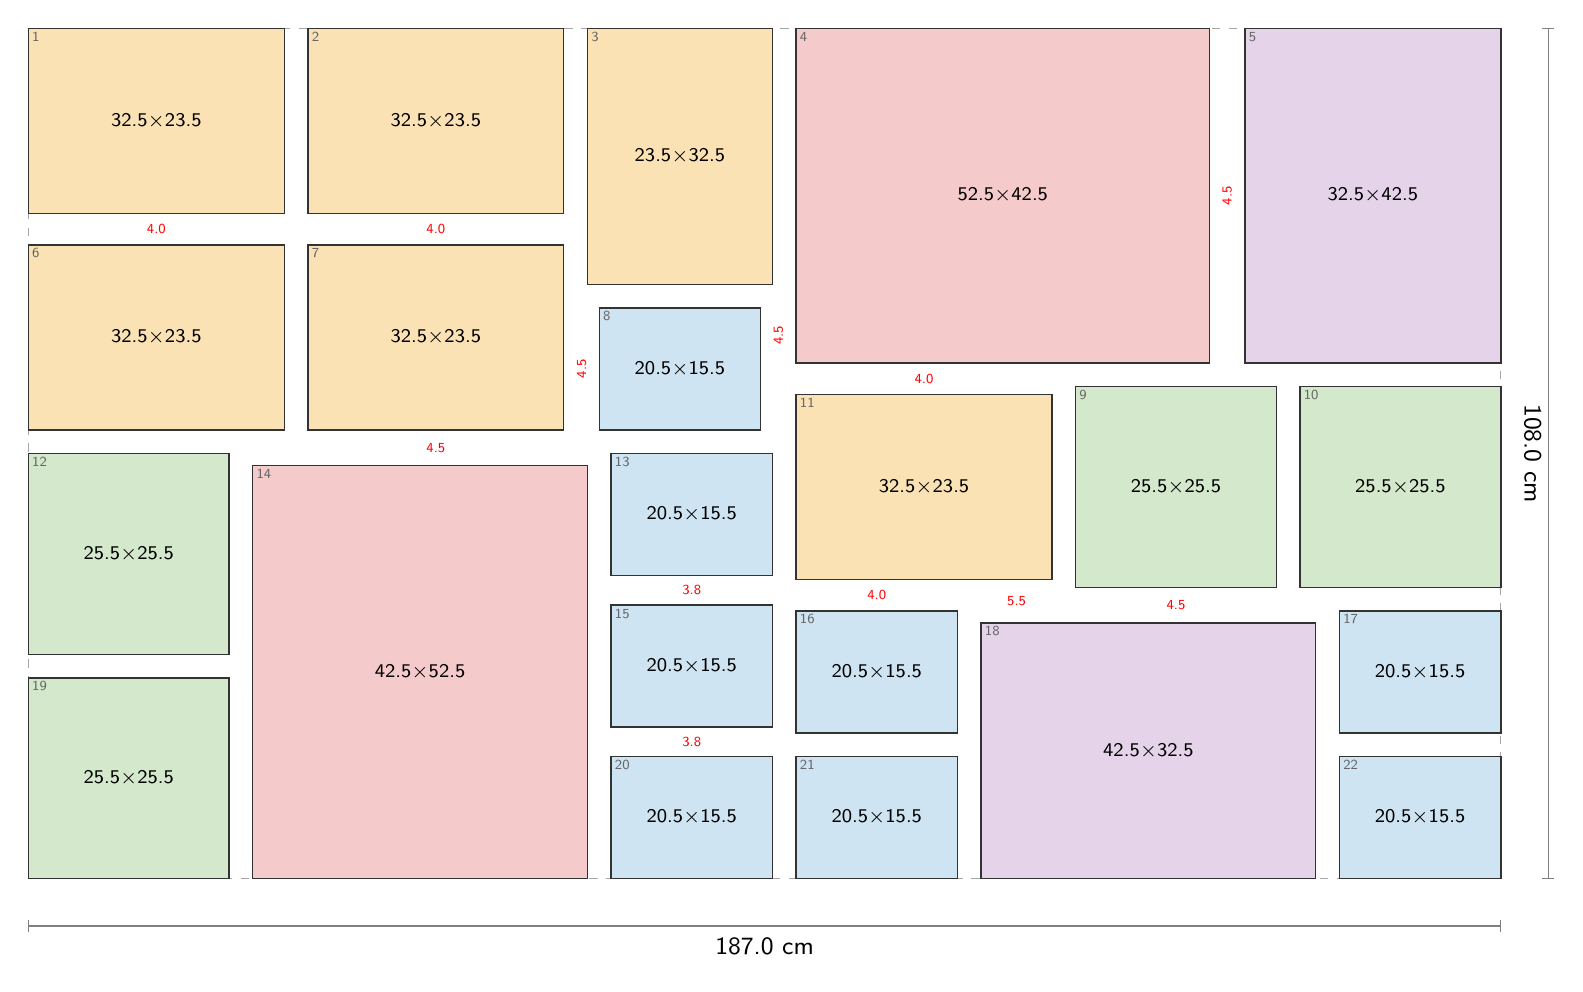
\begin{tikzpicture}[x=1mm, y=-1mm]
\draw[gray!70, dashed, line width=0.4pt] (0,0) rectangle (187.00,108.00);
\filldraw[fill=ft1, draw=black!80, line width=0.5pt] (0.00,0.00) rectangle (32.50,23.50);
\node[align=center, inner sep=0pt] at (16.25,11.75) {\scriptsize 32.5$\times$23.5};
\node[anchor=north west, inner sep=1.2pt, font=\tiny, text=black!60] at (0.00,0.00) {1};
\filldraw[fill=ft1, draw=black!80, line width=0.5pt] (35.50,0.00) rectangle (68.00,23.50);
\node[align=center, inner sep=0pt] at (51.75,11.75) {\scriptsize 32.5$\times$23.5};
\node[anchor=north west, inner sep=1.2pt, font=\tiny, text=black!60] at (35.50,0.00) {2};
\filldraw[fill=ft1, draw=black!80, line width=0.5pt] (71.00,0.00) rectangle (94.50,32.50);
\node[align=center, inner sep=0pt] at (82.75,16.25) {\scriptsize 23.5$\times$32.5};
\node[anchor=north west, inner sep=1.2pt, font=\tiny, text=black!60] at (71.00,0.00) {3};
\filldraw[fill=ft4, draw=black!80, line width=0.5pt] (97.50,0.00) rectangle (150.00,42.50);
\node[align=center, inner sep=0pt] at (123.75,21.25) {\scriptsize 52.5$\times$42.5};
\node[anchor=north west, inner sep=1.2pt, font=\tiny, text=black!60] at (97.50,0.00) {4};
\filldraw[fill=ft3, draw=black!80, line width=0.5pt] (154.50,0.00) rectangle (187.00,42.50);
\node[align=center, inner sep=0pt] at (170.75,21.25) {\scriptsize 32.5$\times$42.5};
\node[anchor=north west, inner sep=1.2pt, font=\tiny, text=black!60] at (154.50,0.00) {5};
\filldraw[fill=ft1, draw=black!80, line width=0.5pt] (0.00,27.50) rectangle (32.50,51.00);
\node[align=center, inner sep=0pt] at (16.25,39.25) {\scriptsize 32.5$\times$23.5};
\node[anchor=north west, inner sep=1.2pt, font=\tiny, text=black!60] at (0.00,27.50) {6};
\filldraw[fill=ft1, draw=black!80, line width=0.5pt] (35.50,27.50) rectangle (68.00,51.00);
\node[align=center, inner sep=0pt] at (51.75,39.25) {\scriptsize 32.5$\times$23.5};
\node[anchor=north west, inner sep=1.2pt, font=\tiny, text=black!60] at (35.50,27.50) {7};
\filldraw[fill=ft0, draw=black!80, line width=0.5pt] (72.50,35.50) rectangle (93.00,51.00);
\node[align=center, inner sep=0pt] at (82.75,43.25) {\scriptsize 20.5$\times$15.5};
\node[anchor=north west, inner sep=1.2pt, font=\tiny, text=black!60] at (72.50,35.50) {8};
\filldraw[fill=ft2, draw=black!80, line width=0.5pt] (133.00,45.50) rectangle (158.50,71.00);
\node[align=center, inner sep=0pt] at (145.75,58.25) {\scriptsize 25.5$\times$25.5};
\node[anchor=north west, inner sep=1.2pt, font=\tiny, text=black!60] at (133.00,45.50) {9};
\filldraw[fill=ft2, draw=black!80, line width=0.5pt] (161.50,45.50) rectangle (187.00,71.00);
\node[align=center, inner sep=0pt] at (174.25,58.25) {\scriptsize 25.5$\times$25.5};
\node[anchor=north west, inner sep=1.2pt, font=\tiny, text=black!60] at (161.50,45.50) {10};
\filldraw[fill=ft1, draw=black!80, line width=0.5pt] (97.50,46.50) rectangle (130.00,70.00);
\node[align=center, inner sep=0pt] at (113.75,58.25) {\scriptsize 32.5$\times$23.5};
\node[anchor=north west, inner sep=1.2pt, font=\tiny, text=black!60] at (97.50,46.50) {11};
\filldraw[fill=ft2, draw=black!80, line width=0.5pt] (0.00,54.00) rectangle (25.50,79.50);
\node[align=center, inner sep=0pt] at (12.75,66.75) {\scriptsize 25.5$\times$25.5};
\node[anchor=north west, inner sep=1.2pt, font=\tiny, text=black!60] at (0.00,54.00) {12};
\filldraw[fill=ft0, draw=black!80, line width=0.5pt] (74.00,54.00) rectangle (94.50,69.50);
\node[align=center, inner sep=0pt] at (84.25,61.75) {\scriptsize 20.5$\times$15.5};
\node[anchor=north west, inner sep=1.2pt, font=\tiny, text=black!60] at (74.00,54.00) {13};
\filldraw[fill=ft4, draw=black!80, line width=0.5pt] (28.50,55.50) rectangle (71.00,108.00);
\node[align=center, inner sep=0pt] at (49.75,81.75) {\scriptsize 42.5$\times$52.5};
\node[anchor=north west, inner sep=1.2pt, font=\tiny, text=black!60] at (28.50,55.50) {14};
\filldraw[fill=ft0, draw=black!80, line width=0.5pt] (74.00,73.25) rectangle (94.50,88.75);
\node[align=center, inner sep=0pt] at (84.25,81.00) {\scriptsize 20.5$\times$15.5};
\node[anchor=north west, inner sep=1.2pt, font=\tiny, text=black!60] at (74.00,73.25) {15};
\filldraw[fill=ft0, draw=black!80, line width=0.5pt] (97.50,74.00) rectangle (118.00,89.50);
\node[align=center, inner sep=0pt] at (107.75,81.75) {\scriptsize 20.5$\times$15.5};
\node[anchor=north west, inner sep=1.2pt, font=\tiny, text=black!60] at (97.50,74.00) {16};
\filldraw[fill=ft0, draw=black!80, line width=0.5pt] (166.50,74.00) rectangle (187.00,89.50);
\node[align=center, inner sep=0pt] at (176.75,81.75) {\scriptsize 20.5$\times$15.5};
\node[anchor=north west, inner sep=1.2pt, font=\tiny, text=black!60] at (166.50,74.00) {17};
\filldraw[fill=ft3, draw=black!80, line width=0.5pt] (121.00,75.50) rectangle (163.50,108.00);
\node[align=center, inner sep=0pt] at (142.25,91.75) {\scriptsize 42.5$\times$32.5};
\node[anchor=north west, inner sep=1.2pt, font=\tiny, text=black!60] at (121.00,75.50) {18};
\filldraw[fill=ft2, draw=black!80, line width=0.5pt] (0.00,82.50) rectangle (25.50,108.00);
\node[align=center, inner sep=0pt] at (12.75,95.25) {\scriptsize 25.5$\times$25.5};
\node[anchor=north west, inner sep=1.2pt, font=\tiny, text=black!60] at (0.00,82.50) {19};
\filldraw[fill=ft0, draw=black!80, line width=0.5pt] (74.00,92.50) rectangle (94.50,108.00);
\node[align=center, inner sep=0pt] at (84.25,100.25) {\scriptsize 20.5$\times$15.5};
\node[anchor=north west, inner sep=1.2pt, font=\tiny, text=black!60] at (74.00,92.50) {20};
\filldraw[fill=ft0, draw=black!80, line width=0.5pt] (97.50,92.50) rectangle (118.00,108.00);
\node[align=center, inner sep=0pt] at (107.75,100.25) {\scriptsize 20.5$\times$15.5};
\node[anchor=north west, inner sep=1.2pt, font=\tiny, text=black!60] at (97.50,92.50) {21};
\filldraw[fill=ft0, draw=black!80, line width=0.5pt] (166.50,92.50) rectangle (187.00,108.00);
\node[align=center, inner sep=0pt] at (176.75,100.25) {\scriptsize 20.5$\times$15.5};
\node[anchor=north west, inner sep=1.2pt, font=\tiny, text=black!60] at (166.50,92.50) {22};
\node[font=\tiny, text=red, fill=white, inner sep=0.3pt] at (16.25,25.50) {4.0};
\node[font=\tiny, text=red, fill=white, inner sep=0.3pt] at (51.75,25.50) {4.0};
\node[font=\tiny, text=red, fill=white, inner sep=0.3pt, rotate=90] at (152.25,21.25) {4.5};
\node[font=\tiny, text=red, fill=white, inner sep=0.3pt] at (113.75,44.50) {4.0};
\node[font=\tiny, text=red, fill=white, inner sep=0.3pt, rotate=90] at (70.25,43.25) {4.5};
\node[font=\tiny, text=red, fill=white, inner sep=0.3pt] at (51.75,53.25) {4.5};
\node[font=\tiny, text=red, fill=white, inner sep=0.3pt, rotate=90] at (95.25,39.00) {4.5};
\node[font=\tiny, text=red, fill=white, inner sep=0.3pt] at (145.75,73.25) {4.5};
\node[font=\tiny, text=red, fill=white, inner sep=0.3pt] at (107.75,72.00) {4.0};
\node[font=\tiny, text=red, fill=white, inner sep=0.3pt] at (125.50,72.75) {5.5};
\node[font=\tiny, text=red, fill=white, inner sep=0.3pt] at (84.25,71.38) {3.8};
\node[font=\tiny, text=red, fill=white, inner sep=0.3pt] at (84.25,90.62) {3.8};
\draw[Bar-Bar, gray] (0,114.00) -- (187.00,114.00) node[midway, below=1pt, font=\small, text=black] {187.0 cm};
\draw[Bar-Bar, gray] (193.00,0) -- (193.00,108.00) node[midway, right=1pt, font=\small, text=black, rotate=-90, anchor=north] {108.0 cm};
\end{tikzpicture}\\[4pt]
{\scriptsize Scale 1:10 (1 mm = 1 cm). Red numbers mark gaps that deviate from the nominal gap by more than 0.25 cm. Small grey numbers index the coordinate table.}
\end{minipage}\hfill
\begin{minipage}[t]{0.25\textwidth}\vspace{0pt}
\small
\begin{tabular}{@{}l l@{}}
\toprule
Outer size & 187.0 $\times$ 108.0 cm \\
Nominal gap & 3 cm \\
Actual gaps & 3.0 -- 5.5 cm \\
Max.\ deviation & 2.5 cm \\
Mean deviation & 0.39 cm \\
Border notches & top 4 cm \\
Corners filled & 4 / 4 \\
Frames used & 22 of 28 \\
\bottomrule
\end{tabular}

\vspace{8pt}
\scriptsize
\begin{tabular}{@{}c l l r r@{}}
\toprule
 & outer w $\times$ h (cm) & & used & have \\
\midrule
\tikz[baseline=-0.6ex]\fill[ft0,draw=black!60] (0,0) rectangle (1.2ex,1.2ex); & 20.5$\times$15.5 & L & 8 & 9 \\
\tikz[baseline=-0.6ex]\fill[ft0,draw=black!60] (0,0) rectangle (1.2ex,1.2ex); & 15.5$\times$20.5 & P & 0 & 2 \\
\tikz[baseline=-0.6ex]\fill[ft3,draw=black!60] (0,0) rectangle (1.2ex,1.2ex); & 32.5$\times$42.5 & P & 1 & 2 \\
\tikz[baseline=-0.6ex]\fill[ft3,draw=black!60] (0,0) rectangle (1.2ex,1.2ex); & 42.5$\times$32.5 & L & 1 & 1 \\
\tikz[baseline=-0.6ex]\fill[ft1,draw=black!60] (0,0) rectangle (1.2ex,1.2ex); & 32.5$\times$23.5 & L & 5 & 5 \\
\tikz[baseline=-0.6ex]\fill[ft1,draw=black!60] (0,0) rectangle (1.2ex,1.2ex); & 23.5$\times$32.5 & P & 1 & 1 \\
\tikz[baseline=-0.6ex]\fill[ft2,draw=black!60] (0,0) rectangle (1.2ex,1.2ex); & 25.5$\times$25.5 &  & 4 & 5 \\
\tikz[baseline=-0.6ex]\fill[ft4,draw=black!60] (0,0) rectangle (1.2ex,1.2ex); & 42.5$\times$52.5 & P & 1 & 1 \\
\tikz[baseline=-0.6ex]\fill[ft4,draw=black!60] (0,0) rectangle (1.2ex,1.2ex); & 52.5$\times$42.5 & L & 1 & 2 \\
\bottomrule
\end{tabular}

\vspace{8pt}
{\bfseries Positions} (top-left corner, cm)\\[2pt]
\tiny
\begin{tabular}{@{}r l r r@{}}
\toprule
\# & frame w $\times$ h & x & y \\
\midrule
1 & 32.5 $\times$ 23.5 & 0.0 & 0.0 \\
2 & 32.5 $\times$ 23.5 & 35.5 & 0.0 \\
3 & 23.5 $\times$ 32.5 & 71.0 & 0.0 \\
4 & 52.5 $\times$ 42.5 & 97.5 & 0.0 \\
5 & 32.5 $\times$ 42.5 & 154.5 & 0.0 \\
6 & 32.5 $\times$ 23.5 & 0.0 & 27.5 \\
7 & 32.5 $\times$ 23.5 & 35.5 & 27.5 \\
8 & 20.5 $\times$ 15.5 & 72.5 & 35.5 \\
9 & 25.5 $\times$ 25.5 & 133.0 & 45.5 \\
10 & 25.5 $\times$ 25.5 & 161.5 & 45.5 \\
11 & 32.5 $\times$ 23.5 & 97.5 & 46.5 \\
12 & 25.5 $\times$ 25.5 & 0.0 & 54.0 \\
13 & 20.5 $\times$ 15.5 & 74.0 & 54.0 \\
14 & 42.5 $\times$ 52.5 & 28.5 & 55.5 \\
15 & 20.5 $\times$ 15.5 & 74.0 & 73.2 \\
16 & 20.5 $\times$ 15.5 & 97.5 & 74.0 \\
17 & 20.5 $\times$ 15.5 & 166.5 & 74.0 \\
18 & 42.5 $\times$ 32.5 & 121.0 & 75.5 \\
19 & 25.5 $\times$ 25.5 & 0.0 & 82.5 \\
20 & 20.5 $\times$ 15.5 & 74.0 & 92.5 \\
21 & 20.5 $\times$ 15.5 & 97.5 & 92.5 \\
22 & 20.5 $\times$ 15.5 & 166.5 & 92.5 \\
\bottomrule
\end{tabular}
\end{minipage}
\clearpage

\begin{minipage}[t]{0.74\textwidth}\vspace{0pt}
{\LARGE\bfseries Layout 9}\hspace{1.5em}{\large 183.5 $\times$ 118.0 cm \quad gap 3 cm \quad 21 frames}\\[8pt]
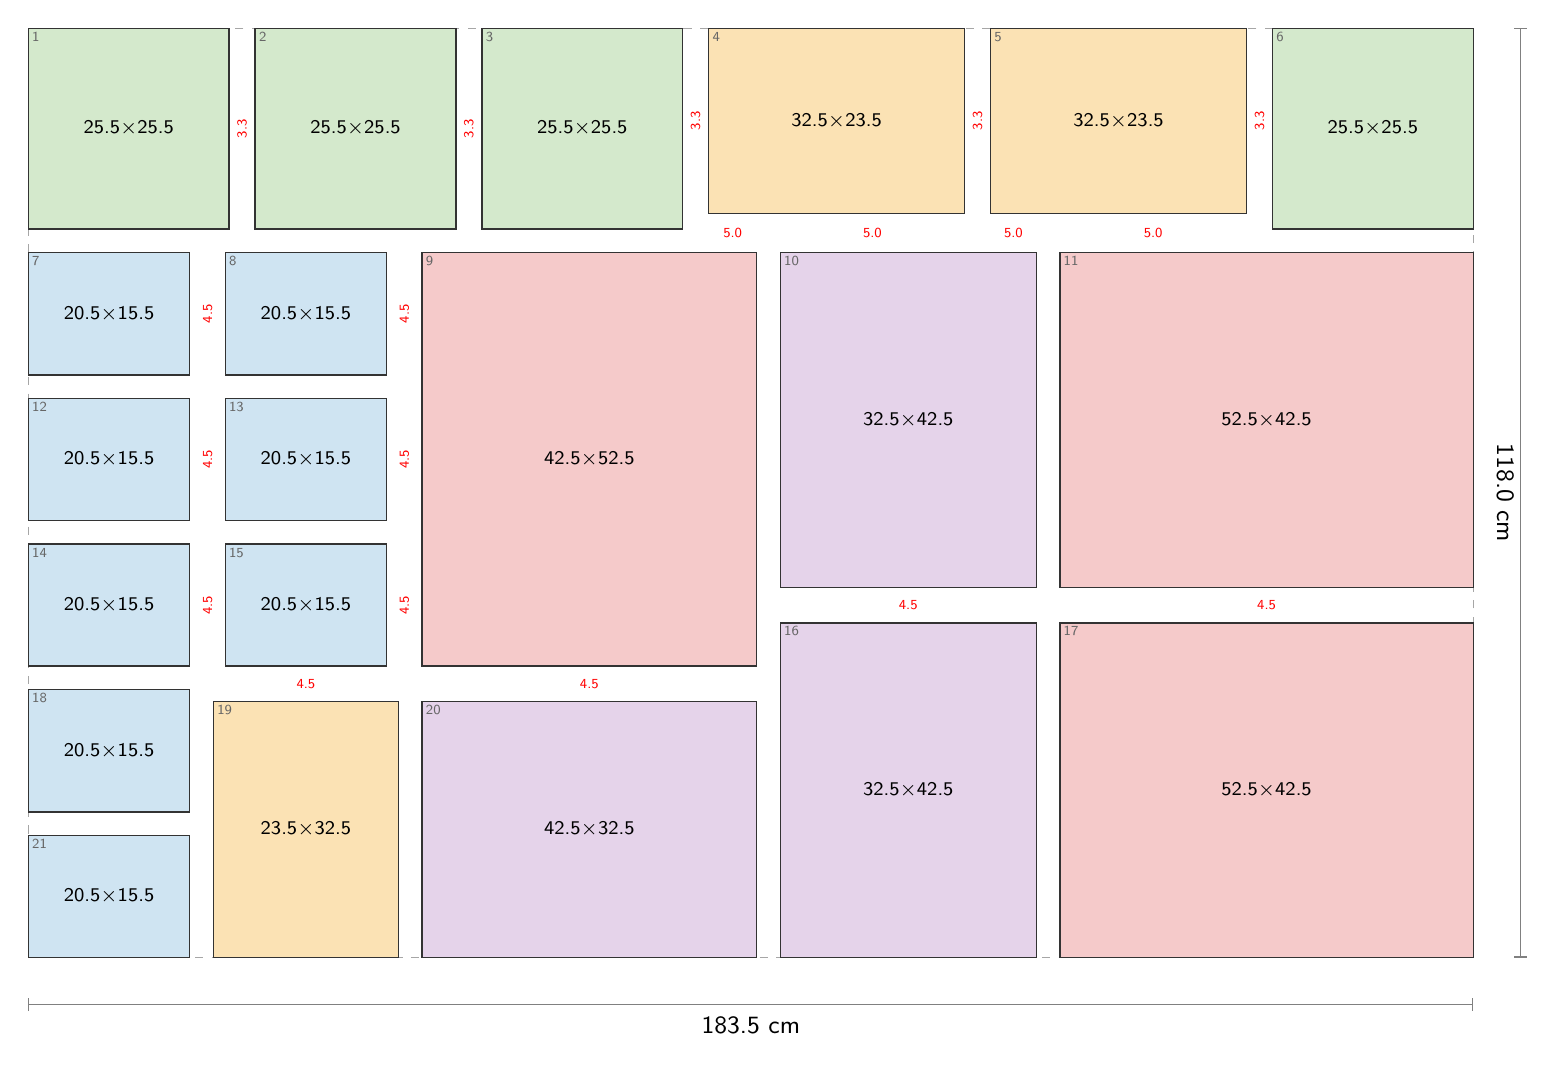
\begin{tikzpicture}[x=1mm, y=-1mm]
\draw[gray!70, dashed, line width=0.4pt] (0,0) rectangle (183.50,118.00);
\filldraw[fill=ft2, draw=black!80, line width=0.5pt] (0.00,0.00) rectangle (25.50,25.50);
\node[align=center, inner sep=0pt] at (12.75,12.75) {\scriptsize 25.5$\times$25.5};
\node[anchor=north west, inner sep=1.2pt, font=\tiny, text=black!60] at (0.00,0.00) {1};
\filldraw[fill=ft2, draw=black!80, line width=0.5pt] (28.80,0.00) rectangle (54.30,25.50);
\node[align=center, inner sep=0pt] at (41.55,12.75) {\scriptsize 25.5$\times$25.5};
\node[anchor=north west, inner sep=1.2pt, font=\tiny, text=black!60] at (28.80,0.00) {2};
\filldraw[fill=ft2, draw=black!80, line width=0.5pt] (57.60,0.00) rectangle (83.10,25.50);
\node[align=center, inner sep=0pt] at (70.35,12.75) {\scriptsize 25.5$\times$25.5};
\node[anchor=north west, inner sep=1.2pt, font=\tiny, text=black!60] at (57.60,0.00) {3};
\filldraw[fill=ft1, draw=black!80, line width=0.5pt] (86.40,0.00) rectangle (118.90,23.50);
\node[align=center, inner sep=0pt] at (102.65,11.75) {\scriptsize 32.5$\times$23.5};
\node[anchor=north west, inner sep=1.2pt, font=\tiny, text=black!60] at (86.40,0.00) {4};
\filldraw[fill=ft1, draw=black!80, line width=0.5pt] (122.20,0.00) rectangle (154.70,23.50);
\node[align=center, inner sep=0pt] at (138.45,11.75) {\scriptsize 32.5$\times$23.5};
\node[anchor=north west, inner sep=1.2pt, font=\tiny, text=black!60] at (122.20,0.00) {5};
\filldraw[fill=ft2, draw=black!80, line width=0.5pt] (158.00,0.00) rectangle (183.50,25.50);
\node[align=center, inner sep=0pt] at (170.75,12.75) {\scriptsize 25.5$\times$25.5};
\node[anchor=north west, inner sep=1.2pt, font=\tiny, text=black!60] at (158.00,0.00) {6};
\filldraw[fill=ft0, draw=black!80, line width=0.5pt] (0.00,28.50) rectangle (20.50,44.00);
\node[align=center, inner sep=0pt] at (10.25,36.25) {\scriptsize 20.5$\times$15.5};
\node[anchor=north west, inner sep=1.2pt, font=\tiny, text=black!60] at (0.00,28.50) {7};
\filldraw[fill=ft0, draw=black!80, line width=0.5pt] (25.00,28.50) rectangle (45.50,44.00);
\node[align=center, inner sep=0pt] at (35.25,36.25) {\scriptsize 20.5$\times$15.5};
\node[anchor=north west, inner sep=1.2pt, font=\tiny, text=black!60] at (25.00,28.50) {8};
\filldraw[fill=ft4, draw=black!80, line width=0.5pt] (50.00,28.50) rectangle (92.50,81.00);
\node[align=center, inner sep=0pt] at (71.25,54.75) {\scriptsize 42.5$\times$52.5};
\node[anchor=north west, inner sep=1.2pt, font=\tiny, text=black!60] at (50.00,28.50) {9};
\filldraw[fill=ft3, draw=black!80, line width=0.5pt] (95.50,28.50) rectangle (128.00,71.00);
\node[align=center, inner sep=0pt] at (111.75,49.75) {\scriptsize 32.5$\times$42.5};
\node[anchor=north west, inner sep=1.2pt, font=\tiny, text=black!60] at (95.50,28.50) {10};
\filldraw[fill=ft4, draw=black!80, line width=0.5pt] (131.00,28.50) rectangle (183.50,71.00);
\node[align=center, inner sep=0pt] at (157.25,49.75) {\scriptsize 52.5$\times$42.5};
\node[anchor=north west, inner sep=1.2pt, font=\tiny, text=black!60] at (131.00,28.50) {11};
\filldraw[fill=ft0, draw=black!80, line width=0.5pt] (0.00,47.00) rectangle (20.50,62.50);
\node[align=center, inner sep=0pt] at (10.25,54.75) {\scriptsize 20.5$\times$15.5};
\node[anchor=north west, inner sep=1.2pt, font=\tiny, text=black!60] at (0.00,47.00) {12};
\filldraw[fill=ft0, draw=black!80, line width=0.5pt] (25.00,47.00) rectangle (45.50,62.50);
\node[align=center, inner sep=0pt] at (35.25,54.75) {\scriptsize 20.5$\times$15.5};
\node[anchor=north west, inner sep=1.2pt, font=\tiny, text=black!60] at (25.00,47.00) {13};
\filldraw[fill=ft0, draw=black!80, line width=0.5pt] (0.00,65.50) rectangle (20.50,81.00);
\node[align=center, inner sep=0pt] at (10.25,73.25) {\scriptsize 20.5$\times$15.5};
\node[anchor=north west, inner sep=1.2pt, font=\tiny, text=black!60] at (0.00,65.50) {14};
\filldraw[fill=ft0, draw=black!80, line width=0.5pt] (25.00,65.50) rectangle (45.50,81.00);
\node[align=center, inner sep=0pt] at (35.25,73.25) {\scriptsize 20.5$\times$15.5};
\node[anchor=north west, inner sep=1.2pt, font=\tiny, text=black!60] at (25.00,65.50) {15};
\filldraw[fill=ft3, draw=black!80, line width=0.5pt] (95.50,75.50) rectangle (128.00,118.00);
\node[align=center, inner sep=0pt] at (111.75,96.75) {\scriptsize 32.5$\times$42.5};
\node[anchor=north west, inner sep=1.2pt, font=\tiny, text=black!60] at (95.50,75.50) {16};
\filldraw[fill=ft4, draw=black!80, line width=0.5pt] (131.00,75.50) rectangle (183.50,118.00);
\node[align=center, inner sep=0pt] at (157.25,96.75) {\scriptsize 52.5$\times$42.5};
\node[anchor=north west, inner sep=1.2pt, font=\tiny, text=black!60] at (131.00,75.50) {17};
\filldraw[fill=ft0, draw=black!80, line width=0.5pt] (0.00,84.00) rectangle (20.50,99.50);
\node[align=center, inner sep=0pt] at (10.25,91.75) {\scriptsize 20.5$\times$15.5};
\node[anchor=north west, inner sep=1.2pt, font=\tiny, text=black!60] at (0.00,84.00) {18};
\filldraw[fill=ft1, draw=black!80, line width=0.5pt] (23.50,85.50) rectangle (47.00,118.00);
\node[align=center, inner sep=0pt] at (35.25,101.75) {\scriptsize 23.5$\times$32.5};
\node[anchor=north west, inner sep=1.2pt, font=\tiny, text=black!60] at (23.50,85.50) {19};
\filldraw[fill=ft3, draw=black!80, line width=0.5pt] (50.00,85.50) rectangle (92.50,118.00);
\node[align=center, inner sep=0pt] at (71.25,101.75) {\scriptsize 42.5$\times$32.5};
\node[anchor=north west, inner sep=1.2pt, font=\tiny, text=black!60] at (50.00,85.50) {20};
\filldraw[fill=ft0, draw=black!80, line width=0.5pt] (0.00,102.50) rectangle (20.50,118.00);
\node[align=center, inner sep=0pt] at (10.25,110.25) {\scriptsize 20.5$\times$15.5};
\node[anchor=north west, inner sep=1.2pt, font=\tiny, text=black!60] at (0.00,102.50) {21};
\node[font=\tiny, text=red, fill=white, inner sep=0.3pt, rotate=90] at (27.15,12.75) {3.3};
\node[font=\tiny, text=red, fill=white, inner sep=0.3pt, rotate=90] at (55.95,12.75) {3.3};
\node[font=\tiny, text=red, fill=white, inner sep=0.3pt, rotate=90] at (84.75,11.75) {3.3};
\node[font=\tiny, text=red, fill=white, inner sep=0.3pt, rotate=90] at (120.55,11.75) {3.3};
\node[font=\tiny, text=red, fill=white, inner sep=0.3pt] at (89.45,26.00) {5.0};
\node[font=\tiny, text=red, fill=white, inner sep=0.3pt] at (107.20,26.00) {5.0};
\node[font=\tiny, text=red, fill=white, inner sep=0.3pt, rotate=90] at (156.35,11.75) {3.3};
\node[font=\tiny, text=red, fill=white, inner sep=0.3pt] at (125.10,26.00) {5.0};
\node[font=\tiny, text=red, fill=white, inner sep=0.3pt] at (142.85,26.00) {5.0};
\node[font=\tiny, text=red, fill=white, inner sep=0.3pt, rotate=90] at (22.75,36.25) {4.5};
\node[font=\tiny, text=red, fill=white, inner sep=0.3pt, rotate=90] at (47.75,36.25) {4.5};
\node[font=\tiny, text=red, fill=white, inner sep=0.3pt] at (71.25,83.25) {4.5};
\node[font=\tiny, text=red, fill=white, inner sep=0.3pt] at (111.75,73.25) {4.5};
\node[font=\tiny, text=red, fill=white, inner sep=0.3pt] at (157.25,73.25) {4.5};
\node[font=\tiny, text=red, fill=white, inner sep=0.3pt, rotate=90] at (22.75,54.75) {4.5};
\node[font=\tiny, text=red, fill=white, inner sep=0.3pt, rotate=90] at (47.75,54.75) {4.5};
\node[font=\tiny, text=red, fill=white, inner sep=0.3pt, rotate=90] at (22.75,73.25) {4.5};
\node[font=\tiny, text=red, fill=white, inner sep=0.3pt, rotate=90] at (47.75,73.25) {4.5};
\node[font=\tiny, text=red, fill=white, inner sep=0.3pt] at (35.25,83.25) {4.5};
\draw[Bar-Bar, gray] (0,124.00) -- (183.50,124.00) node[midway, below=1pt, font=\small, text=black] {183.5 cm};
\draw[Bar-Bar, gray] (189.50,0) -- (189.50,118.00) node[midway, right=1pt, font=\small, text=black, rotate=-90, anchor=north] {118.0 cm};
\end{tikzpicture}\\[4pt]
{\scriptsize Scale 1:10 (1 mm = 1 cm). Red numbers mark gaps that deviate from the nominal gap by more than 0.25 cm. Small grey numbers index the coordinate table.}
\end{minipage}\hfill
\begin{minipage}[t]{0.25\textwidth}\vspace{0pt}
\small
\begin{tabular}{@{}l l@{}}
\toprule
Outer size & 183.5 $\times$ 118.0 cm \\
Nominal gap & 3 cm \\
Actual gaps & 3.0 -- 5.0 cm \\
Max.\ deviation & 2.0 cm \\
Mean deviation & 0.66 cm \\
Border notches & right 4 cm \\
Corners filled & 4 / 4 \\
Frames used & 21 of 28 \\
\bottomrule
\end{tabular}

\vspace{8pt}
\scriptsize
\begin{tabular}{@{}c l l r r@{}}
\toprule
 & outer w $\times$ h (cm) & & used & have \\
\midrule
\tikz[baseline=-0.6ex]\fill[ft0,draw=black!60] (0,0) rectangle (1.2ex,1.2ex); & 20.5$\times$15.5 & L & 8 & 9 \\
\tikz[baseline=-0.6ex]\fill[ft0,draw=black!60] (0,0) rectangle (1.2ex,1.2ex); & 15.5$\times$20.5 & P & 0 & 2 \\
\tikz[baseline=-0.6ex]\fill[ft3,draw=black!60] (0,0) rectangle (1.2ex,1.2ex); & 32.5$\times$42.5 & P & 2 & 2 \\
\tikz[baseline=-0.6ex]\fill[ft3,draw=black!60] (0,0) rectangle (1.2ex,1.2ex); & 42.5$\times$32.5 & L & 1 & 1 \\
\tikz[baseline=-0.6ex]\fill[ft1,draw=black!60] (0,0) rectangle (1.2ex,1.2ex); & 32.5$\times$23.5 & L & 2 & 5 \\
\tikz[baseline=-0.6ex]\fill[ft1,draw=black!60] (0,0) rectangle (1.2ex,1.2ex); & 23.5$\times$32.5 & P & 1 & 1 \\
\tikz[baseline=-0.6ex]\fill[ft2,draw=black!60] (0,0) rectangle (1.2ex,1.2ex); & 25.5$\times$25.5 &  & 4 & 5 \\
\tikz[baseline=-0.6ex]\fill[ft4,draw=black!60] (0,0) rectangle (1.2ex,1.2ex); & 42.5$\times$52.5 & P & 1 & 1 \\
\tikz[baseline=-0.6ex]\fill[ft4,draw=black!60] (0,0) rectangle (1.2ex,1.2ex); & 52.5$\times$42.5 & L & 2 & 2 \\
\bottomrule
\end{tabular}

\vspace{8pt}
{\bfseries Positions} (top-left corner, cm)\\[2pt]
\tiny
\begin{tabular}{@{}r l r r@{}}
\toprule
\# & frame w $\times$ h & x & y \\
\midrule
1 & 25.5 $\times$ 25.5 & 0.0 & 0.0 \\
2 & 25.5 $\times$ 25.5 & 28.8 & 0.0 \\
3 & 25.5 $\times$ 25.5 & 57.6 & 0.0 \\
4 & 32.5 $\times$ 23.5 & 86.4 & 0.0 \\
5 & 32.5 $\times$ 23.5 & 122.2 & 0.0 \\
6 & 25.5 $\times$ 25.5 & 158.0 & 0.0 \\
7 & 20.5 $\times$ 15.5 & 0.0 & 28.5 \\
8 & 20.5 $\times$ 15.5 & 25.0 & 28.5 \\
9 & 42.5 $\times$ 52.5 & 50.0 & 28.5 \\
10 & 32.5 $\times$ 42.5 & 95.5 & 28.5 \\
11 & 52.5 $\times$ 42.5 & 131.0 & 28.5 \\
12 & 20.5 $\times$ 15.5 & 0.0 & 47.0 \\
13 & 20.5 $\times$ 15.5 & 25.0 & 47.0 \\
14 & 20.5 $\times$ 15.5 & 0.0 & 65.5 \\
15 & 20.5 $\times$ 15.5 & 25.0 & 65.5 \\
16 & 32.5 $\times$ 42.5 & 95.5 & 75.5 \\
17 & 52.5 $\times$ 42.5 & 131.0 & 75.5 \\
18 & 20.5 $\times$ 15.5 & 0.0 & 84.0 \\
19 & 23.5 $\times$ 32.5 & 23.5 & 85.5 \\
20 & 42.5 $\times$ 32.5 & 50.0 & 85.5 \\
21 & 20.5 $\times$ 15.5 & 0.0 & 102.5 \\
\bottomrule
\end{tabular}
\end{minipage}
\clearpage

\begin{minipage}[t]{0.74\textwidth}\vspace{0pt}
{\LARGE\bfseries Layout 10}\hspace{1.5em}{\large 179.0 $\times$ 126.0 cm \quad gap 3 cm \quad 25 frames}\\[8pt]
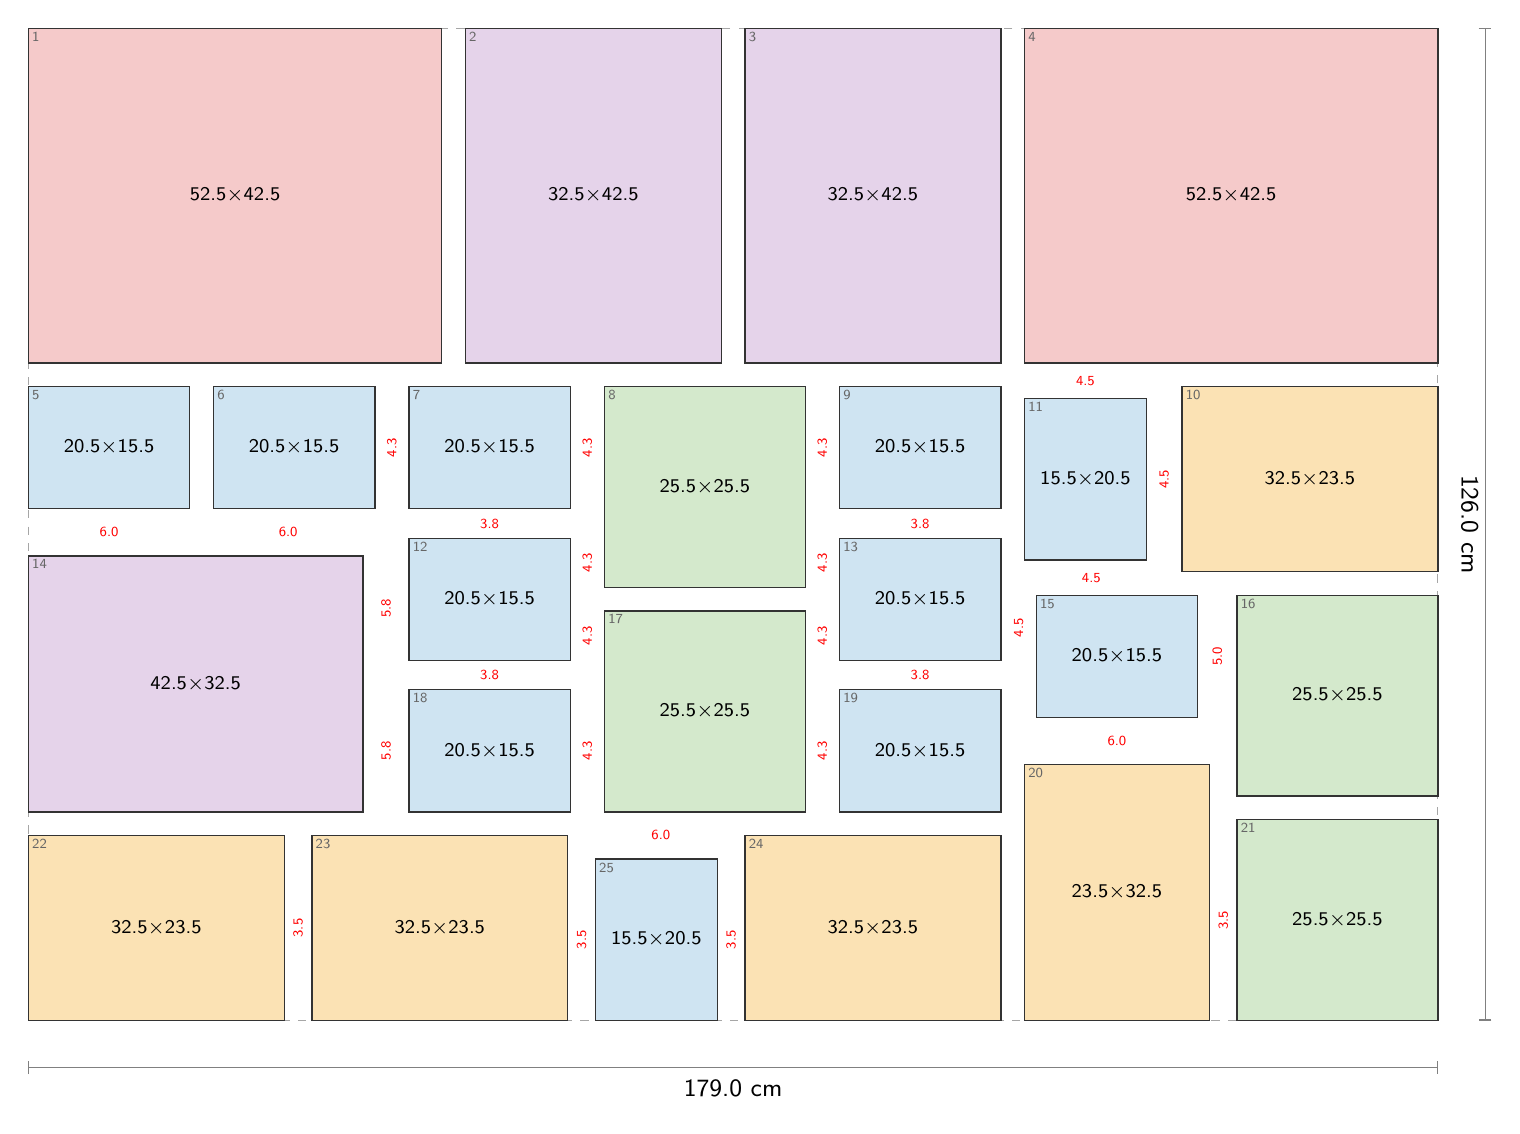
\begin{tikzpicture}[x=1mm, y=-1mm]
\draw[gray!70, dashed, line width=0.4pt] (0,0) rectangle (179.00,126.00);
\filldraw[fill=ft4, draw=black!80, line width=0.5pt] (0.00,0.00) rectangle (52.50,42.50);
\node[align=center, inner sep=0pt] at (26.25,21.25) {\scriptsize 52.5$\times$42.5};
\node[anchor=north west, inner sep=1.2pt, font=\tiny, text=black!60] at (0.00,0.00) {1};
\filldraw[fill=ft3, draw=black!80, line width=0.5pt] (55.50,0.00) rectangle (88.00,42.50);
\node[align=center, inner sep=0pt] at (71.75,21.25) {\scriptsize 32.5$\times$42.5};
\node[anchor=north west, inner sep=1.2pt, font=\tiny, text=black!60] at (55.50,0.00) {2};
\filldraw[fill=ft3, draw=black!80, line width=0.5pt] (91.00,0.00) rectangle (123.50,42.50);
\node[align=center, inner sep=0pt] at (107.25,21.25) {\scriptsize 32.5$\times$42.5};
\node[anchor=north west, inner sep=1.2pt, font=\tiny, text=black!60] at (91.00,0.00) {3};
\filldraw[fill=ft4, draw=black!80, line width=0.5pt] (126.50,0.00) rectangle (179.00,42.50);
\node[align=center, inner sep=0pt] at (152.75,21.25) {\scriptsize 52.5$\times$42.5};
\node[anchor=north west, inner sep=1.2pt, font=\tiny, text=black!60] at (126.50,0.00) {4};
\filldraw[fill=ft0, draw=black!80, line width=0.5pt] (0.00,45.50) rectangle (20.50,61.00);
\node[align=center, inner sep=0pt] at (10.25,53.25) {\scriptsize 20.5$\times$15.5};
\node[anchor=north west, inner sep=1.2pt, font=\tiny, text=black!60] at (0.00,45.50) {5};
\filldraw[fill=ft0, draw=black!80, line width=0.5pt] (23.50,45.50) rectangle (44.00,61.00);
\node[align=center, inner sep=0pt] at (33.75,53.25) {\scriptsize 20.5$\times$15.5};
\node[anchor=north west, inner sep=1.2pt, font=\tiny, text=black!60] at (23.50,45.50) {6};
\filldraw[fill=ft0, draw=black!80, line width=0.5pt] (48.33,45.50) rectangle (68.83,61.00);
\node[align=center, inner sep=0pt] at (58.58,53.25) {\scriptsize 20.5$\times$15.5};
\node[anchor=north west, inner sep=1.2pt, font=\tiny, text=black!60] at (48.33,45.50) {7};
\filldraw[fill=ft2, draw=black!80, line width=0.5pt] (73.17,45.50) rectangle (98.67,71.00);
\node[align=center, inner sep=0pt] at (85.92,58.25) {\scriptsize 25.5$\times$25.5};
\node[anchor=north west, inner sep=1.2pt, font=\tiny, text=black!60] at (73.17,45.50) {8};
\filldraw[fill=ft0, draw=black!80, line width=0.5pt] (103.00,45.50) rectangle (123.50,61.00);
\node[align=center, inner sep=0pt] at (113.25,53.25) {\scriptsize 20.5$\times$15.5};
\node[anchor=north west, inner sep=1.2pt, font=\tiny, text=black!60] at (103.00,45.50) {9};
\filldraw[fill=ft1, draw=black!80, line width=0.5pt] (146.50,45.50) rectangle (179.00,69.00);
\node[align=center, inner sep=0pt] at (162.75,57.25) {\scriptsize 32.5$\times$23.5};
\node[anchor=north west, inner sep=1.2pt, font=\tiny, text=black!60] at (146.50,45.50) {10};
\filldraw[fill=ft0, draw=black!80, line width=0.5pt] (126.50,47.00) rectangle (142.00,67.50);
\node[align=center, inner sep=0pt] at (134.25,57.25) {\scriptsize 15.5$\times$20.5};
\node[anchor=north west, inner sep=1.2pt, font=\tiny, text=black!60] at (126.50,47.00) {11};
\filldraw[fill=ft0, draw=black!80, line width=0.5pt] (48.33,64.75) rectangle (68.83,80.25);
\node[align=center, inner sep=0pt] at (58.58,72.50) {\scriptsize 20.5$\times$15.5};
\node[anchor=north west, inner sep=1.2pt, font=\tiny, text=black!60] at (48.33,64.75) {12};
\filldraw[fill=ft0, draw=black!80, line width=0.5pt] (103.00,64.75) rectangle (123.50,80.25);
\node[align=center, inner sep=0pt] at (113.25,72.50) {\scriptsize 20.5$\times$15.5};
\node[anchor=north west, inner sep=1.2pt, font=\tiny, text=black!60] at (103.00,64.75) {13};
\filldraw[fill=ft3, draw=black!80, line width=0.5pt] (0.00,67.00) rectangle (42.50,99.50);
\node[align=center, inner sep=0pt] at (21.25,83.25) {\scriptsize 42.5$\times$32.5};
\node[anchor=north west, inner sep=1.2pt, font=\tiny, text=black!60] at (0.00,67.00) {14};
\filldraw[fill=ft0, draw=black!80, line width=0.5pt] (128.00,72.00) rectangle (148.50,87.50);
\node[align=center, inner sep=0pt] at (138.25,79.75) {\scriptsize 20.5$\times$15.5};
\node[anchor=north west, inner sep=1.2pt, font=\tiny, text=black!60] at (128.00,72.00) {15};
\filldraw[fill=ft2, draw=black!80, line width=0.5pt] (153.50,72.00) rectangle (179.00,97.50);
\node[align=center, inner sep=0pt] at (166.25,84.75) {\scriptsize 25.5$\times$25.5};
\node[anchor=north west, inner sep=1.2pt, font=\tiny, text=black!60] at (153.50,72.00) {16};
\filldraw[fill=ft2, draw=black!80, line width=0.5pt] (73.17,74.00) rectangle (98.67,99.50);
\node[align=center, inner sep=0pt] at (85.92,86.75) {\scriptsize 25.5$\times$25.5};
\node[anchor=north west, inner sep=1.2pt, font=\tiny, text=black!60] at (73.17,74.00) {17};
\filldraw[fill=ft0, draw=black!80, line width=0.5pt] (48.33,84.00) rectangle (68.83,99.50);
\node[align=center, inner sep=0pt] at (58.58,91.75) {\scriptsize 20.5$\times$15.5};
\node[anchor=north west, inner sep=1.2pt, font=\tiny, text=black!60] at (48.33,84.00) {18};
\filldraw[fill=ft0, draw=black!80, line width=0.5pt] (103.00,84.00) rectangle (123.50,99.50);
\node[align=center, inner sep=0pt] at (113.25,91.75) {\scriptsize 20.5$\times$15.5};
\node[anchor=north west, inner sep=1.2pt, font=\tiny, text=black!60] at (103.00,84.00) {19};
\filldraw[fill=ft1, draw=black!80, line width=0.5pt] (126.50,93.50) rectangle (150.00,126.00);
\node[align=center, inner sep=0pt] at (138.25,109.75) {\scriptsize 23.5$\times$32.5};
\node[anchor=north west, inner sep=1.2pt, font=\tiny, text=black!60] at (126.50,93.50) {20};
\filldraw[fill=ft2, draw=black!80, line width=0.5pt] (153.50,100.50) rectangle (179.00,126.00);
\node[align=center, inner sep=0pt] at (166.25,113.25) {\scriptsize 25.5$\times$25.5};
\node[anchor=north west, inner sep=1.2pt, font=\tiny, text=black!60] at (153.50,100.50) {21};
\filldraw[fill=ft1, draw=black!80, line width=0.5pt] (0.00,102.50) rectangle (32.50,126.00);
\node[align=center, inner sep=0pt] at (16.25,114.25) {\scriptsize 32.5$\times$23.5};
\node[anchor=north west, inner sep=1.2pt, font=\tiny, text=black!60] at (0.00,102.50) {22};
\filldraw[fill=ft1, draw=black!80, line width=0.5pt] (36.00,102.50) rectangle (68.50,126.00);
\node[align=center, inner sep=0pt] at (52.25,114.25) {\scriptsize 32.5$\times$23.5};
\node[anchor=north west, inner sep=1.2pt, font=\tiny, text=black!60] at (36.00,102.50) {23};
\filldraw[fill=ft1, draw=black!80, line width=0.5pt] (91.00,102.50) rectangle (123.50,126.00);
\node[align=center, inner sep=0pt] at (107.25,114.25) {\scriptsize 32.5$\times$23.5};
\node[anchor=north west, inner sep=1.2pt, font=\tiny, text=black!60] at (91.00,102.50) {24};
\filldraw[fill=ft0, draw=black!80, line width=0.5pt] (72.00,105.50) rectangle (87.50,126.00);
\node[align=center, inner sep=0pt] at (79.75,115.75) {\scriptsize 15.5$\times$20.5};
\node[anchor=north west, inner sep=1.2pt, font=\tiny, text=black!60] at (72.00,105.50) {25};
\node[font=\tiny, text=red, fill=white, inner sep=0.3pt] at (134.25,44.75) {4.5};
\node[font=\tiny, text=red, fill=white, inner sep=0.3pt] at (10.25,64.00) {6.0};
\node[font=\tiny, text=red, fill=white, inner sep=0.3pt, rotate=90] at (46.17,53.25) {4.3};
\node[font=\tiny, text=red, fill=white, inner sep=0.3pt] at (33.00,64.00) {6.0};
\node[font=\tiny, text=red, fill=white, inner sep=0.3pt, rotate=90] at (71.00,53.25) {4.3};
\node[font=\tiny, text=red, fill=white, inner sep=0.3pt] at (58.58,62.88) {3.8};
\node[font=\tiny, text=red, fill=white, inner sep=0.3pt, rotate=90] at (100.83,53.25) {4.3};
\node[font=\tiny, text=red, fill=white, inner sep=0.3pt, rotate=90] at (100.83,67.88) {4.3};
\node[font=\tiny, text=red, fill=white, inner sep=0.3pt] at (113.25,62.88) {3.8};
\node[font=\tiny, text=red, fill=white, inner sep=0.3pt, rotate=90] at (144.25,57.25) {4.5};
\node[font=\tiny, text=red, fill=white, inner sep=0.3pt] at (135.00,69.75) {4.5};
\node[font=\tiny, text=red, fill=white, inner sep=0.3pt, rotate=90] at (71.00,67.88) {4.3};
\node[font=\tiny, text=red, fill=white, inner sep=0.3pt, rotate=90] at (71.00,77.12) {4.3};
\node[font=\tiny, text=red, fill=white, inner sep=0.3pt] at (58.58,82.12) {3.8};
\node[font=\tiny, text=red, fill=white, inner sep=0.3pt, rotate=90] at (125.75,76.12) {4.5};
\node[font=\tiny, text=red, fill=white, inner sep=0.3pt] at (113.25,82.12) {3.8};
\node[font=\tiny, text=red, fill=white, inner sep=0.3pt, rotate=90] at (45.42,73.62) {5.8};
\node[font=\tiny, text=red, fill=white, inner sep=0.3pt, rotate=90] at (45.42,91.75) {5.8};
\node[font=\tiny, text=red, fill=white, inner sep=0.3pt, rotate=90] at (151.00,79.75) {5.0};
\node[font=\tiny, text=red, fill=white, inner sep=0.3pt] at (138.25,90.50) {6.0};
\node[font=\tiny, text=red, fill=white, inner sep=0.3pt, rotate=90] at (100.83,77.12) {4.3};
\node[font=\tiny, text=red, fill=white, inner sep=0.3pt, rotate=90] at (100.83,91.75) {4.3};
\node[font=\tiny, text=red, fill=white, inner sep=0.3pt] at (80.33,102.50) {6.0};
\node[font=\tiny, text=red, fill=white, inner sep=0.3pt, rotate=90] at (71.00,91.75) {4.3};
\node[font=\tiny, text=red, fill=white, inner sep=0.3pt, rotate=90] at (151.75,113.25) {3.5};
\node[font=\tiny, text=red, fill=white, inner sep=0.3pt, rotate=90] at (34.25,114.25) {3.5};
\node[font=\tiny, text=red, fill=white, inner sep=0.3pt, rotate=90] at (70.25,115.75) {3.5};
\node[font=\tiny, text=red, fill=white, inner sep=0.3pt, rotate=90] at (89.25,115.75) {3.5};
\draw[Bar-Bar, gray] (0,132.00) -- (179.00,132.00) node[midway, below=1pt, font=\small, text=black] {179.0 cm};
\draw[Bar-Bar, gray] (185.00,0) -- (185.00,126.00) node[midway, right=1pt, font=\small, text=black, rotate=-90, anchor=north] {126.0 cm};
\end{tikzpicture}\\[4pt]
{\scriptsize Scale 1:10 (1 mm = 1 cm). Red numbers mark gaps that deviate from the nominal gap by more than 0.25 cm. Small grey numbers index the coordinate table.}
\end{minipage}\hfill
\begin{minipage}[t]{0.25\textwidth}\vspace{0pt}
\small
\begin{tabular}{@{}l l@{}}
\toprule
Outer size & 179.0 $\times$ 126.0 cm \\
Nominal gap & 3 cm \\
Actual gaps & 3.0 -- 6.0 cm \\
Max.\ deviation & 3.0 cm \\
Mean deviation & 0.85 cm \\
Border notches & left 6 cm \\
Corners filled & 4 / 4 \\
Frames used & 25 of 28 \\
\bottomrule
\end{tabular}

\vspace{8pt}
\scriptsize
\begin{tabular}{@{}c l l r r@{}}
\toprule
 & outer w $\times$ h (cm) & & used & have \\
\midrule
\tikz[baseline=-0.6ex]\fill[ft0,draw=black!60] (0,0) rectangle (1.2ex,1.2ex); & 20.5$\times$15.5 & L & 9 & 9 \\
\tikz[baseline=-0.6ex]\fill[ft0,draw=black!60] (0,0) rectangle (1.2ex,1.2ex); & 15.5$\times$20.5 & P & 2 & 2 \\
\tikz[baseline=-0.6ex]\fill[ft3,draw=black!60] (0,0) rectangle (1.2ex,1.2ex); & 32.5$\times$42.5 & P & 2 & 2 \\
\tikz[baseline=-0.6ex]\fill[ft3,draw=black!60] (0,0) rectangle (1.2ex,1.2ex); & 42.5$\times$32.5 & L & 1 & 1 \\
\tikz[baseline=-0.6ex]\fill[ft1,draw=black!60] (0,0) rectangle (1.2ex,1.2ex); & 32.5$\times$23.5 & L & 4 & 5 \\
\tikz[baseline=-0.6ex]\fill[ft1,draw=black!60] (0,0) rectangle (1.2ex,1.2ex); & 23.5$\times$32.5 & P & 1 & 1 \\
\tikz[baseline=-0.6ex]\fill[ft2,draw=black!60] (0,0) rectangle (1.2ex,1.2ex); & 25.5$\times$25.5 &  & 4 & 5 \\
\tikz[baseline=-0.6ex]\fill[ft4,draw=black!60] (0,0) rectangle (1.2ex,1.2ex); & 42.5$\times$52.5 & P & 0 & 1 \\
\tikz[baseline=-0.6ex]\fill[ft4,draw=black!60] (0,0) rectangle (1.2ex,1.2ex); & 52.5$\times$42.5 & L & 2 & 2 \\
\bottomrule
\end{tabular}

\vspace{8pt}
{\bfseries Positions} (top-left corner, cm)\\[2pt]
\tiny
\begin{tabular}{@{}r l r r@{}}
\toprule
\# & frame w $\times$ h & x & y \\
\midrule
1 & 52.5 $\times$ 42.5 & 0.0 & 0.0 \\
2 & 32.5 $\times$ 42.5 & 55.5 & 0.0 \\
3 & 32.5 $\times$ 42.5 & 91.0 & 0.0 \\
4 & 52.5 $\times$ 42.5 & 126.5 & 0.0 \\
5 & 20.5 $\times$ 15.5 & 0.0 & 45.5 \\
6 & 20.5 $\times$ 15.5 & 23.5 & 45.5 \\
7 & 20.5 $\times$ 15.5 & 48.3 & 45.5 \\
8 & 25.5 $\times$ 25.5 & 73.2 & 45.5 \\
9 & 20.5 $\times$ 15.5 & 103.0 & 45.5 \\
10 & 32.5 $\times$ 23.5 & 146.5 & 45.5 \\
11 & 15.5 $\times$ 20.5 & 126.5 & 47.0 \\
12 & 20.5 $\times$ 15.5 & 48.3 & 64.8 \\
13 & 20.5 $\times$ 15.5 & 103.0 & 64.8 \\
14 & 42.5 $\times$ 32.5 & 0.0 & 67.0 \\
15 & 20.5 $\times$ 15.5 & 128.0 & 72.0 \\
16 & 25.5 $\times$ 25.5 & 153.5 & 72.0 \\
17 & 25.5 $\times$ 25.5 & 73.2 & 74.0 \\
18 & 20.5 $\times$ 15.5 & 48.3 & 84.0 \\
19 & 20.5 $\times$ 15.5 & 103.0 & 84.0 \\
20 & 23.5 $\times$ 32.5 & 126.5 & 93.5 \\
21 & 25.5 $\times$ 25.5 & 153.5 & 100.5 \\
22 & 32.5 $\times$ 23.5 & 0.0 & 102.5 \\
23 & 32.5 $\times$ 23.5 & 36.0 & 102.5 \\
24 & 32.5 $\times$ 23.5 & 91.0 & 102.5 \\
25 & 15.5 $\times$ 20.5 & 72.0 & 105.5 \\
\bottomrule
\end{tabular}
\end{minipage}
\clearpage

\begin{minipage}[t]{0.74\textwidth}\vspace{0pt}
{\LARGE\bfseries Layout 11}\hspace{1.5em}{\large 181.5 $\times$ 125.0 cm \quad gap 3 cm \quad 25 frames}\\[8pt]
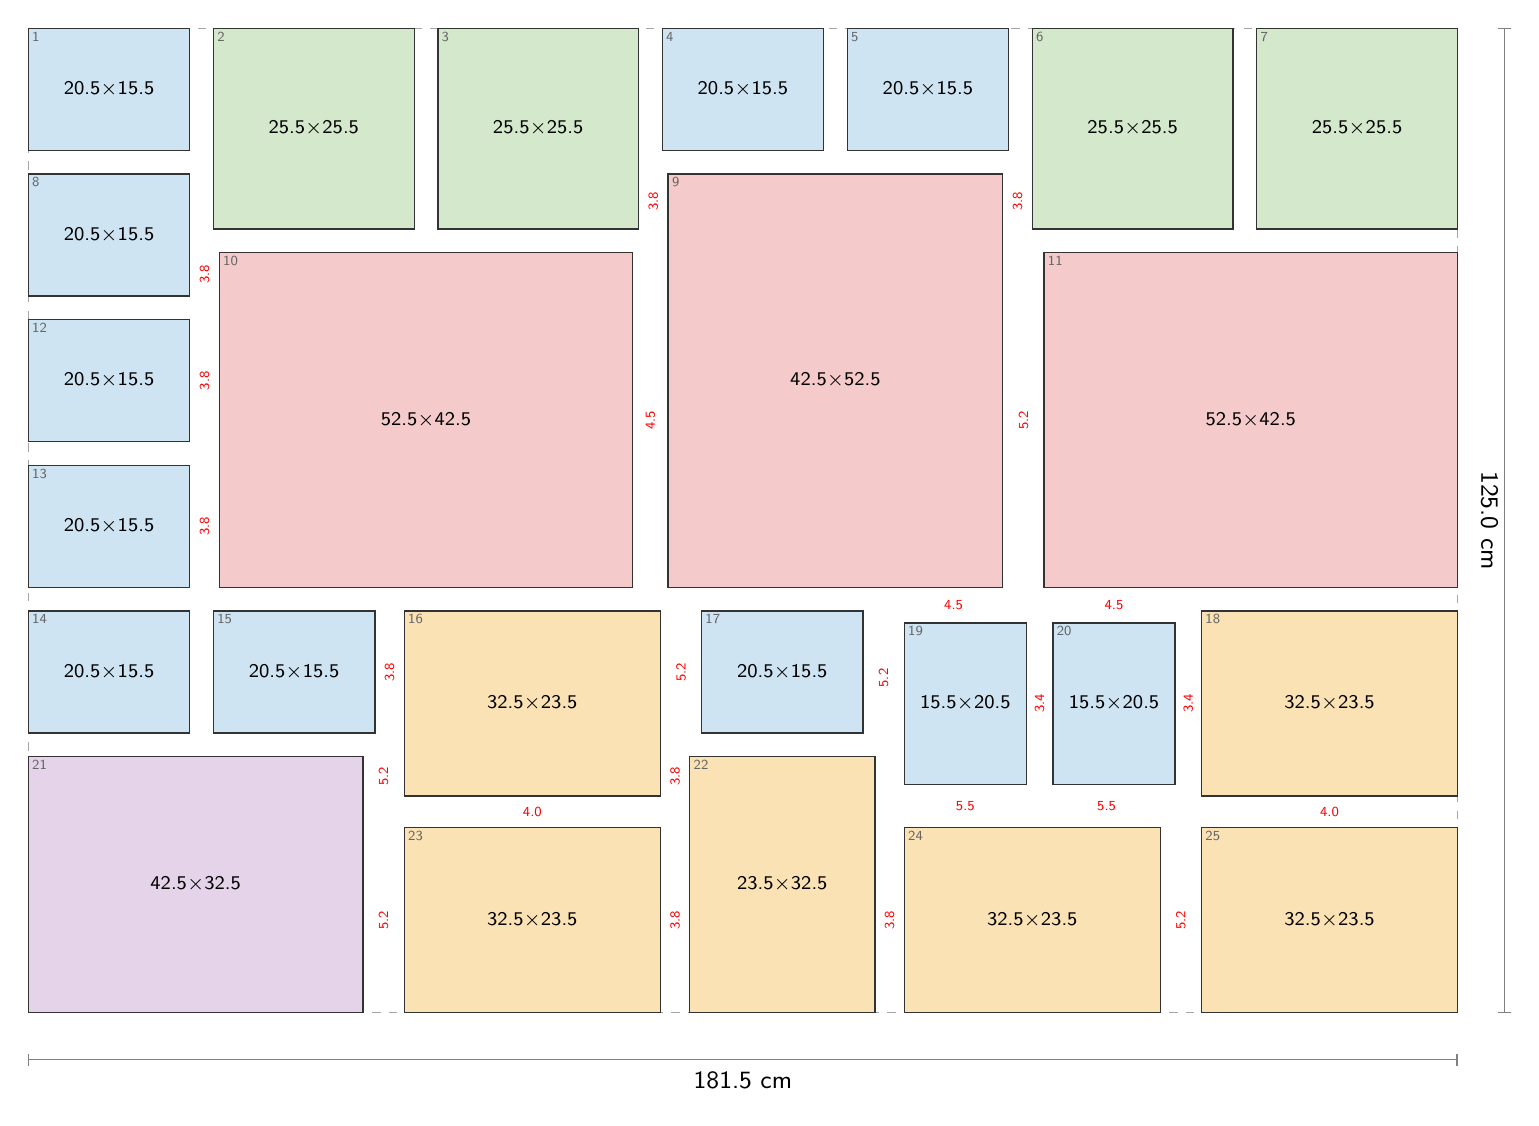
\begin{tikzpicture}[x=1mm, y=-1mm]
\draw[gray!70, dashed, line width=0.4pt] (0,0) rectangle (181.50,125.00);
\filldraw[fill=ft0, draw=black!80, line width=0.5pt] (0.00,0.00) rectangle (20.50,15.50);
\node[align=center, inner sep=0pt] at (10.25,7.75) {\scriptsize 20.5$\times$15.5};
\node[anchor=north west, inner sep=1.2pt, font=\tiny, text=black!60] at (0.00,0.00) {1};
\filldraw[fill=ft2, draw=black!80, line width=0.5pt] (23.50,0.00) rectangle (49.00,25.50);
\node[align=center, inner sep=0pt] at (36.25,12.75) {\scriptsize 25.5$\times$25.5};
\node[anchor=north west, inner sep=1.2pt, font=\tiny, text=black!60] at (23.50,0.00) {2};
\filldraw[fill=ft2, draw=black!80, line width=0.5pt] (52.00,0.00) rectangle (77.50,25.50);
\node[align=center, inner sep=0pt] at (64.75,12.75) {\scriptsize 25.5$\times$25.5};
\node[anchor=north west, inner sep=1.2pt, font=\tiny, text=black!60] at (52.00,0.00) {3};
\filldraw[fill=ft0, draw=black!80, line width=0.5pt] (80.50,0.00) rectangle (101.00,15.50);
\node[align=center, inner sep=0pt] at (90.75,7.75) {\scriptsize 20.5$\times$15.5};
\node[anchor=north west, inner sep=1.2pt, font=\tiny, text=black!60] at (80.50,0.00) {4};
\filldraw[fill=ft0, draw=black!80, line width=0.5pt] (104.00,0.00) rectangle (124.50,15.50);
\node[align=center, inner sep=0pt] at (114.25,7.75) {\scriptsize 20.5$\times$15.5};
\node[anchor=north west, inner sep=1.2pt, font=\tiny, text=black!60] at (104.00,0.00) {5};
\filldraw[fill=ft2, draw=black!80, line width=0.5pt] (127.50,0.00) rectangle (153.00,25.50);
\node[align=center, inner sep=0pt] at (140.25,12.75) {\scriptsize 25.5$\times$25.5};
\node[anchor=north west, inner sep=1.2pt, font=\tiny, text=black!60] at (127.50,0.00) {6};
\filldraw[fill=ft2, draw=black!80, line width=0.5pt] (156.00,0.00) rectangle (181.50,25.50);
\node[align=center, inner sep=0pt] at (168.75,12.75) {\scriptsize 25.5$\times$25.5};
\node[anchor=north west, inner sep=1.2pt, font=\tiny, text=black!60] at (156.00,0.00) {7};
\filldraw[fill=ft0, draw=black!80, line width=0.5pt] (0.00,18.50) rectangle (20.50,34.00);
\node[align=center, inner sep=0pt] at (10.25,26.25) {\scriptsize 20.5$\times$15.5};
\node[anchor=north west, inner sep=1.2pt, font=\tiny, text=black!60] at (0.00,18.50) {8};
\filldraw[fill=ft4, draw=black!80, line width=0.5pt] (81.25,18.50) rectangle (123.75,71.00);
\node[align=center, inner sep=0pt] at (102.50,44.75) {\scriptsize 42.5$\times$52.5};
\node[anchor=north west, inner sep=1.2pt, font=\tiny, text=black!60] at (81.25,18.50) {9};
\filldraw[fill=ft4, draw=black!80, line width=0.5pt] (24.25,28.50) rectangle (76.75,71.00);
\node[align=center, inner sep=0pt] at (50.50,49.75) {\scriptsize 52.5$\times$42.5};
\node[anchor=north west, inner sep=1.2pt, font=\tiny, text=black!60] at (24.25,28.50) {10};
\filldraw[fill=ft4, draw=black!80, line width=0.5pt] (129.00,28.50) rectangle (181.50,71.00);
\node[align=center, inner sep=0pt] at (155.25,49.75) {\scriptsize 52.5$\times$42.5};
\node[anchor=north west, inner sep=1.2pt, font=\tiny, text=black!60] at (129.00,28.50) {11};
\filldraw[fill=ft0, draw=black!80, line width=0.5pt] (0.00,37.00) rectangle (20.50,52.50);
\node[align=center, inner sep=0pt] at (10.25,44.75) {\scriptsize 20.5$\times$15.5};
\node[anchor=north west, inner sep=1.2pt, font=\tiny, text=black!60] at (0.00,37.00) {12};
\filldraw[fill=ft0, draw=black!80, line width=0.5pt] (0.00,55.50) rectangle (20.50,71.00);
\node[align=center, inner sep=0pt] at (10.25,63.25) {\scriptsize 20.5$\times$15.5};
\node[anchor=north west, inner sep=1.2pt, font=\tiny, text=black!60] at (0.00,55.50) {13};
\filldraw[fill=ft0, draw=black!80, line width=0.5pt] (0.00,74.00) rectangle (20.50,89.50);
\node[align=center, inner sep=0pt] at (10.25,81.75) {\scriptsize 20.5$\times$15.5};
\node[anchor=north west, inner sep=1.2pt, font=\tiny, text=black!60] at (0.00,74.00) {14};
\filldraw[fill=ft0, draw=black!80, line width=0.5pt] (23.50,74.00) rectangle (44.00,89.50);
\node[align=center, inner sep=0pt] at (33.75,81.75) {\scriptsize 20.5$\times$15.5};
\node[anchor=north west, inner sep=1.2pt, font=\tiny, text=black!60] at (23.50,74.00) {15};
\filldraw[fill=ft1, draw=black!80, line width=0.5pt] (47.75,74.00) rectangle (80.25,97.50);
\node[align=center, inner sep=0pt] at (64.00,85.75) {\scriptsize 32.5$\times$23.5};
\node[anchor=north west, inner sep=1.2pt, font=\tiny, text=black!60] at (47.75,74.00) {16};
\filldraw[fill=ft0, draw=black!80, line width=0.5pt] (85.50,74.00) rectangle (106.00,89.50);
\node[align=center, inner sep=0pt] at (95.75,81.75) {\scriptsize 20.5$\times$15.5};
\node[anchor=north west, inner sep=1.2pt, font=\tiny, text=black!60] at (85.50,74.00) {17};
\filldraw[fill=ft1, draw=black!80, line width=0.5pt] (149.00,74.00) rectangle (181.50,97.50);
\node[align=center, inner sep=0pt] at (165.25,85.75) {\scriptsize 32.5$\times$23.5};
\node[anchor=north west, inner sep=1.2pt, font=\tiny, text=black!60] at (149.00,74.00) {18};
\filldraw[fill=ft0, draw=black!80, line width=0.5pt] (111.25,75.50) rectangle (126.75,96.00);
\node[align=center, inner sep=0pt] at (119.00,85.75) {\scriptsize 15.5$\times$20.5};
\node[anchor=north west, inner sep=1.2pt, font=\tiny, text=black!60] at (111.25,75.50) {19};
\filldraw[fill=ft0, draw=black!80, line width=0.5pt] (130.12,75.50) rectangle (145.62,96.00);
\node[align=center, inner sep=0pt] at (137.88,85.75) {\scriptsize 15.5$\times$20.5};
\node[anchor=north west, inner sep=1.2pt, font=\tiny, text=black!60] at (130.12,75.50) {20};
\filldraw[fill=ft3, draw=black!80, line width=0.5pt] (0.00,92.50) rectangle (42.50,125.00);
\node[align=center, inner sep=0pt] at (21.25,108.75) {\scriptsize 42.5$\times$32.5};
\node[anchor=north west, inner sep=1.2pt, font=\tiny, text=black!60] at (0.00,92.50) {21};
\filldraw[fill=ft1, draw=black!80, line width=0.5pt] (84.00,92.50) rectangle (107.50,125.00);
\node[align=center, inner sep=0pt] at (95.75,108.75) {\scriptsize 23.5$\times$32.5};
\node[anchor=north west, inner sep=1.2pt, font=\tiny, text=black!60] at (84.00,92.50) {22};
\filldraw[fill=ft1, draw=black!80, line width=0.5pt] (47.75,101.50) rectangle (80.25,125.00);
\node[align=center, inner sep=0pt] at (64.00,113.25) {\scriptsize 32.5$\times$23.5};
\node[anchor=north west, inner sep=1.2pt, font=\tiny, text=black!60] at (47.75,101.50) {23};
\filldraw[fill=ft1, draw=black!80, line width=0.5pt] (111.25,101.50) rectangle (143.75,125.00);
\node[align=center, inner sep=0pt] at (127.50,113.25) {\scriptsize 32.5$\times$23.5};
\node[anchor=north west, inner sep=1.2pt, font=\tiny, text=black!60] at (111.25,101.50) {24};
\filldraw[fill=ft1, draw=black!80, line width=0.5pt] (149.00,101.50) rectangle (181.50,125.00);
\node[align=center, inner sep=0pt] at (165.25,113.25) {\scriptsize 32.5$\times$23.5};
\node[anchor=north west, inner sep=1.2pt, font=\tiny, text=black!60] at (149.00,101.50) {25};
\node[font=\tiny, text=red, fill=white, inner sep=0.3pt, rotate=90] at (79.38,22.00) {3.8};
\node[font=\tiny, text=red, fill=white, inner sep=0.3pt, rotate=90] at (22.38,31.25) {3.8};
\node[font=\tiny, text=red, fill=white, inner sep=0.3pt, rotate=90] at (125.62,22.00) {3.8};
\node[font=\tiny, text=red, fill=white, inner sep=0.3pt, rotate=90] at (126.38,49.75) {5.2};
\node[font=\tiny, text=red, fill=white, inner sep=0.3pt] at (117.50,73.25) {4.5};
\node[font=\tiny, text=red, fill=white, inner sep=0.3pt, rotate=90] at (79.00,49.75) {4.5};
\node[font=\tiny, text=red, fill=white, inner sep=0.3pt] at (137.88,73.25) {4.5};
\node[font=\tiny, text=red, fill=white, inner sep=0.3pt, rotate=90] at (22.38,44.75) {3.8};
\node[font=\tiny, text=red, fill=white, inner sep=0.3pt, rotate=90] at (22.38,63.25) {3.8};
\node[font=\tiny, text=red, fill=white, inner sep=0.3pt, rotate=90] at (45.88,81.75) {3.8};
\node[font=\tiny, text=red, fill=white, inner sep=0.3pt, rotate=90] at (82.88,81.75) {5.2};
\node[font=\tiny, text=red, fill=white, inner sep=0.3pt, rotate=90] at (82.12,95.00) {3.8};
\node[font=\tiny, text=red, fill=white, inner sep=0.3pt] at (64.00,99.50) {4.0};
\node[font=\tiny, text=red, fill=white, inner sep=0.3pt, rotate=90] at (108.62,82.50) {5.2};
\node[font=\tiny, text=red, fill=white, inner sep=0.3pt] at (165.25,99.50) {4.0};
\node[font=\tiny, text=red, fill=white, inner sep=0.3pt, rotate=90] at (128.44,85.75) {3.4};
\node[font=\tiny, text=red, fill=white, inner sep=0.3pt] at (119.00,98.75) {5.5};
\node[font=\tiny, text=red, fill=white, inner sep=0.3pt, rotate=90] at (147.31,85.75) {3.4};
\node[font=\tiny, text=red, fill=white, inner sep=0.3pt] at (136.94,98.75) {5.5};
\node[font=\tiny, text=red, fill=white, inner sep=0.3pt, rotate=90] at (45.12,95.00) {5.2};
\node[font=\tiny, text=red, fill=white, inner sep=0.3pt, rotate=90] at (45.12,113.25) {5.2};
\node[font=\tiny, text=red, fill=white, inner sep=0.3pt, rotate=90] at (109.38,113.25) {3.8};
\node[font=\tiny, text=red, fill=white, inner sep=0.3pt, rotate=90] at (82.12,113.25) {3.8};
\node[font=\tiny, text=red, fill=white, inner sep=0.3pt, rotate=90] at (146.38,113.25) {5.2};
\draw[Bar-Bar, gray] (0,131.00) -- (181.50,131.00) node[midway, below=1pt, font=\small, text=black] {181.5 cm};
\draw[Bar-Bar, gray] (187.50,0) -- (187.50,125.00) node[midway, right=1pt, font=\small, text=black, rotate=-90, anchor=north] {125.0 cm};
\end{tikzpicture}\\[4pt]
{\scriptsize Scale 1:10 (1 mm = 1 cm). Red numbers mark gaps that deviate from the nominal gap by more than 0.25 cm. Small grey numbers index the coordinate table.}
\end{minipage}\hfill
\begin{minipage}[t]{0.25\textwidth}\vspace{0pt}
\small
\begin{tabular}{@{}l l@{}}
\toprule
Outer size & 181.5 $\times$ 125.0 cm \\
Nominal gap & 3 cm \\
Actual gaps & 3.0 -- 5.5 cm \\
Max.\ deviation & 2.5 cm \\
Mean deviation & 0.66 cm \\
Border notches & bottom 10 cm \\
Corners filled & 4 / 4 \\
Frames used & 25 of 28 \\
\bottomrule
\end{tabular}

\vspace{8pt}
\scriptsize
\begin{tabular}{@{}c l l r r@{}}
\toprule
 & outer w $\times$ h (cm) & & used & have \\
\midrule
\tikz[baseline=-0.6ex]\fill[ft0,draw=black!60] (0,0) rectangle (1.2ex,1.2ex); & 20.5$\times$15.5 & L & 9 & 9 \\
\tikz[baseline=-0.6ex]\fill[ft0,draw=black!60] (0,0) rectangle (1.2ex,1.2ex); & 15.5$\times$20.5 & P & 2 & 2 \\
\tikz[baseline=-0.6ex]\fill[ft3,draw=black!60] (0,0) rectangle (1.2ex,1.2ex); & 32.5$\times$42.5 & P & 0 & 2 \\
\tikz[baseline=-0.6ex]\fill[ft3,draw=black!60] (0,0) rectangle (1.2ex,1.2ex); & 42.5$\times$32.5 & L & 1 & 1 \\
\tikz[baseline=-0.6ex]\fill[ft1,draw=black!60] (0,0) rectangle (1.2ex,1.2ex); & 32.5$\times$23.5 & L & 5 & 5 \\
\tikz[baseline=-0.6ex]\fill[ft1,draw=black!60] (0,0) rectangle (1.2ex,1.2ex); & 23.5$\times$32.5 & P & 1 & 1 \\
\tikz[baseline=-0.6ex]\fill[ft2,draw=black!60] (0,0) rectangle (1.2ex,1.2ex); & 25.5$\times$25.5 &  & 4 & 5 \\
\tikz[baseline=-0.6ex]\fill[ft4,draw=black!60] (0,0) rectangle (1.2ex,1.2ex); & 42.5$\times$52.5 & P & 1 & 1 \\
\tikz[baseline=-0.6ex]\fill[ft4,draw=black!60] (0,0) rectangle (1.2ex,1.2ex); & 52.5$\times$42.5 & L & 2 & 2 \\
\bottomrule
\end{tabular}

\vspace{8pt}
{\bfseries Positions} (top-left corner, cm)\\[2pt]
\tiny
\begin{tabular}{@{}r l r r@{}}
\toprule
\# & frame w $\times$ h & x & y \\
\midrule
1 & 20.5 $\times$ 15.5 & 0.0 & 0.0 \\
2 & 25.5 $\times$ 25.5 & 23.5 & 0.0 \\
3 & 25.5 $\times$ 25.5 & 52.0 & 0.0 \\
4 & 20.5 $\times$ 15.5 & 80.5 & 0.0 \\
5 & 20.5 $\times$ 15.5 & 104.0 & 0.0 \\
6 & 25.5 $\times$ 25.5 & 127.5 & 0.0 \\
7 & 25.5 $\times$ 25.5 & 156.0 & 0.0 \\
8 & 20.5 $\times$ 15.5 & 0.0 & 18.5 \\
9 & 42.5 $\times$ 52.5 & 81.2 & 18.5 \\
10 & 52.5 $\times$ 42.5 & 24.2 & 28.5 \\
11 & 52.5 $\times$ 42.5 & 129.0 & 28.5 \\
12 & 20.5 $\times$ 15.5 & 0.0 & 37.0 \\
13 & 20.5 $\times$ 15.5 & 0.0 & 55.5 \\
14 & 20.5 $\times$ 15.5 & 0.0 & 74.0 \\
15 & 20.5 $\times$ 15.5 & 23.5 & 74.0 \\
16 & 32.5 $\times$ 23.5 & 47.8 & 74.0 \\
17 & 20.5 $\times$ 15.5 & 85.5 & 74.0 \\
18 & 32.5 $\times$ 23.5 & 149.0 & 74.0 \\
19 & 15.5 $\times$ 20.5 & 111.2 & 75.5 \\
20 & 15.5 $\times$ 20.5 & 130.1 & 75.5 \\
21 & 42.5 $\times$ 32.5 & 0.0 & 92.5 \\
22 & 23.5 $\times$ 32.5 & 84.0 & 92.5 \\
23 & 32.5 $\times$ 23.5 & 47.8 & 101.5 \\
24 & 32.5 $\times$ 23.5 & 111.2 & 101.5 \\
25 & 32.5 $\times$ 23.5 & 149.0 & 101.5 \\
\bottomrule
\end{tabular}
\end{minipage}
\clearpage

\begin{minipage}[t]{0.74\textwidth}\vspace{0pt}
{\LARGE\bfseries Layout 12}\hspace{1.5em}{\large 181.5 $\times$ 128.0 cm \quad gap 3 cm \quad 25 frames}\\[8pt]
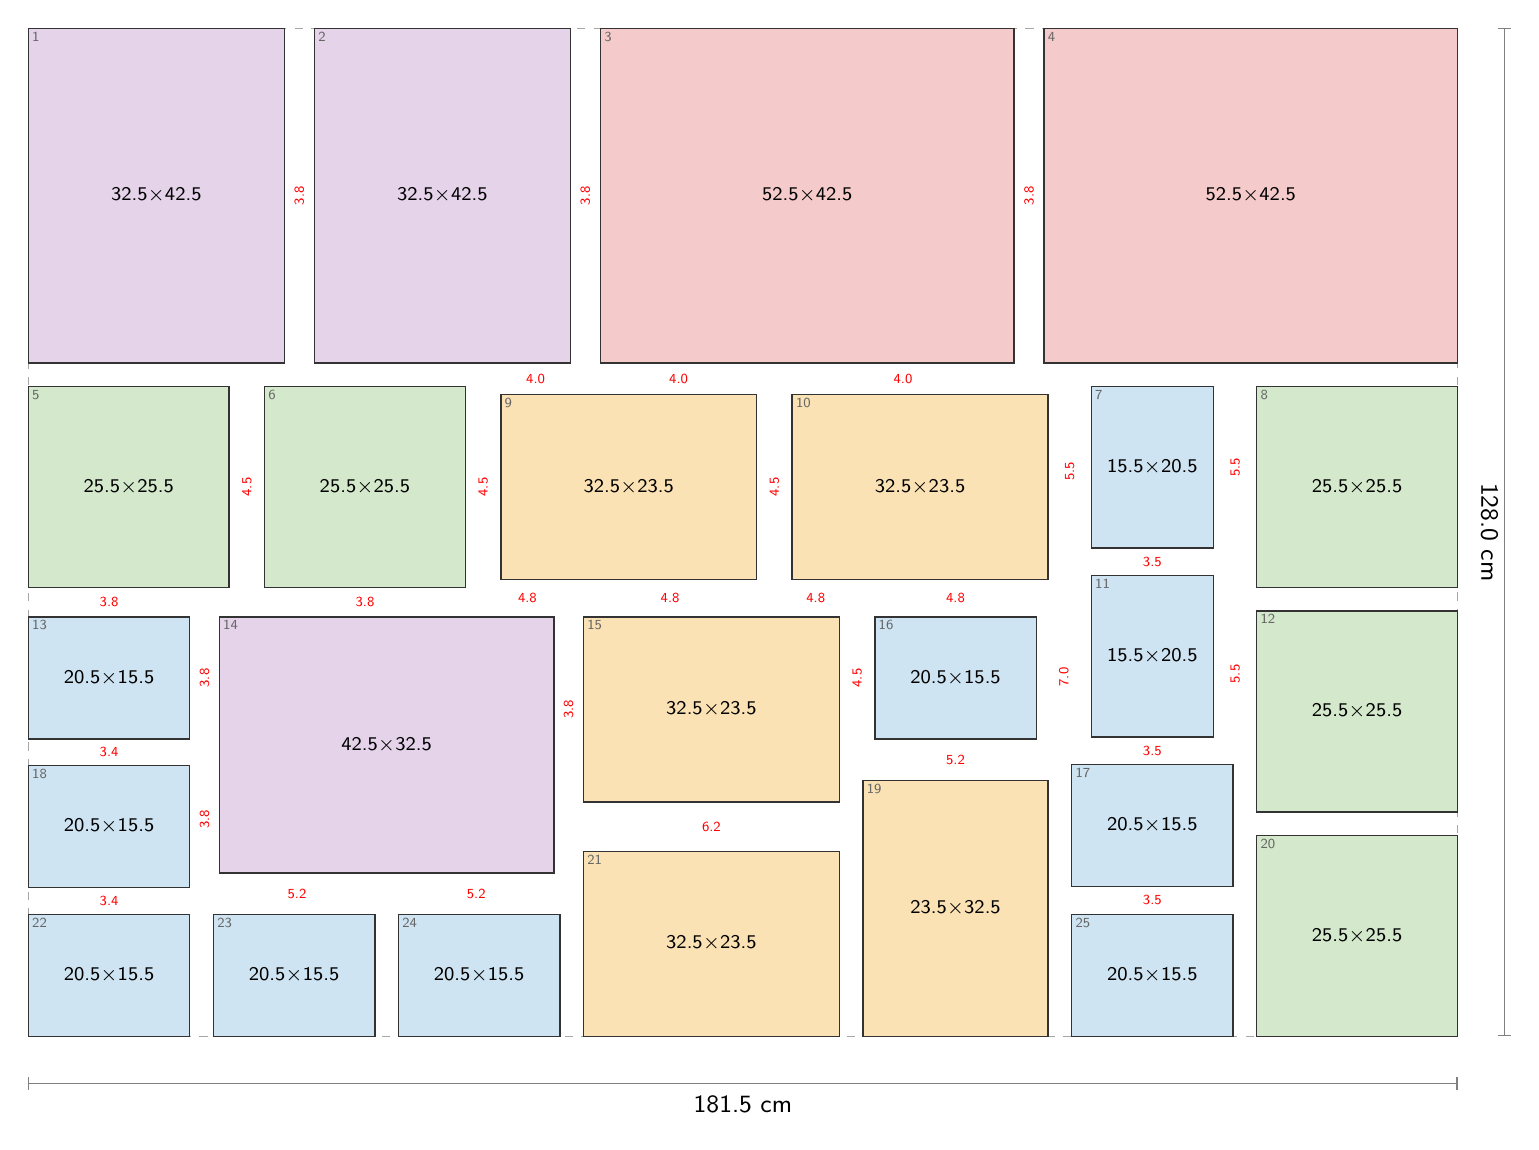
\begin{tikzpicture}[x=1mm, y=-1mm]
\draw[gray!70, dashed, line width=0.4pt] (0,0) rectangle (181.50,128.00);
\filldraw[fill=ft3, draw=black!80, line width=0.5pt] (0.00,0.00) rectangle (32.50,42.50);
\node[align=center, inner sep=0pt] at (16.25,21.25) {\scriptsize 32.5$\times$42.5};
\node[anchor=north west, inner sep=1.2pt, font=\tiny, text=black!60] at (0.00,0.00) {1};
\filldraw[fill=ft3, draw=black!80, line width=0.5pt] (36.33,0.00) rectangle (68.83,42.50);
\node[align=center, inner sep=0pt] at (52.58,21.25) {\scriptsize 32.5$\times$42.5};
\node[anchor=north west, inner sep=1.2pt, font=\tiny, text=black!60] at (36.33,0.00) {2};
\filldraw[fill=ft4, draw=black!80, line width=0.5pt] (72.67,0.00) rectangle (125.17,42.50);
\node[align=center, inner sep=0pt] at (98.92,21.25) {\scriptsize 52.5$\times$42.5};
\node[anchor=north west, inner sep=1.2pt, font=\tiny, text=black!60] at (72.67,0.00) {3};
\filldraw[fill=ft4, draw=black!80, line width=0.5pt] (129.00,0.00) rectangle (181.50,42.50);
\node[align=center, inner sep=0pt] at (155.25,21.25) {\scriptsize 52.5$\times$42.5};
\node[anchor=north west, inner sep=1.2pt, font=\tiny, text=black!60] at (129.00,0.00) {4};
\filldraw[fill=ft2, draw=black!80, line width=0.5pt] (0.00,45.50) rectangle (25.50,71.00);
\node[align=center, inner sep=0pt] at (12.75,58.25) {\scriptsize 25.5$\times$25.5};
\node[anchor=north west, inner sep=1.2pt, font=\tiny, text=black!60] at (0.00,45.50) {5};
\filldraw[fill=ft2, draw=black!80, line width=0.5pt] (30.00,45.50) rectangle (55.50,71.00);
\node[align=center, inner sep=0pt] at (42.75,58.25) {\scriptsize 25.5$\times$25.5};
\node[anchor=north west, inner sep=1.2pt, font=\tiny, text=black!60] at (30.00,45.50) {6};
\filldraw[fill=ft0, draw=black!80, line width=0.5pt] (135.00,45.50) rectangle (150.50,66.00);
\node[align=center, inner sep=0pt] at (142.75,55.75) {\scriptsize 15.5$\times$20.5};
\node[anchor=north west, inner sep=1.2pt, font=\tiny, text=black!60] at (135.00,45.50) {7};
\filldraw[fill=ft2, draw=black!80, line width=0.5pt] (156.00,45.50) rectangle (181.50,71.00);
\node[align=center, inner sep=0pt] at (168.75,58.25) {\scriptsize 25.5$\times$25.5};
\node[anchor=north west, inner sep=1.2pt, font=\tiny, text=black!60] at (156.00,45.50) {8};
\filldraw[fill=ft1, draw=black!80, line width=0.5pt] (60.00,46.50) rectangle (92.50,70.00);
\node[align=center, inner sep=0pt] at (76.25,58.25) {\scriptsize 32.5$\times$23.5};
\node[anchor=north west, inner sep=1.2pt, font=\tiny, text=black!60] at (60.00,46.50) {9};
\filldraw[fill=ft1, draw=black!80, line width=0.5pt] (97.00,46.50) rectangle (129.50,70.00);
\node[align=center, inner sep=0pt] at (113.25,58.25) {\scriptsize 32.5$\times$23.5};
\node[anchor=north west, inner sep=1.2pt, font=\tiny, text=black!60] at (97.00,46.50) {10};
\filldraw[fill=ft0, draw=black!80, line width=0.5pt] (135.00,69.50) rectangle (150.50,90.00);
\node[align=center, inner sep=0pt] at (142.75,79.75) {\scriptsize 15.5$\times$20.5};
\node[anchor=north west, inner sep=1.2pt, font=\tiny, text=black!60] at (135.00,69.50) {11};
\filldraw[fill=ft2, draw=black!80, line width=0.5pt] (156.00,74.00) rectangle (181.50,99.50);
\node[align=center, inner sep=0pt] at (168.75,86.75) {\scriptsize 25.5$\times$25.5};
\node[anchor=north west, inner sep=1.2pt, font=\tiny, text=black!60] at (156.00,74.00) {12};
\filldraw[fill=ft0, draw=black!80, line width=0.5pt] (0.00,74.75) rectangle (20.50,90.25);
\node[align=center, inner sep=0pt] at (10.25,82.50) {\scriptsize 20.5$\times$15.5};
\node[anchor=north west, inner sep=1.2pt, font=\tiny, text=black!60] at (0.00,74.75) {13};
\filldraw[fill=ft3, draw=black!80, line width=0.5pt] (24.25,74.75) rectangle (66.75,107.25);
\node[align=center, inner sep=0pt] at (45.50,91.00) {\scriptsize 42.5$\times$32.5};
\node[anchor=north west, inner sep=1.2pt, font=\tiny, text=black!60] at (24.25,74.75) {14};
\filldraw[fill=ft1, draw=black!80, line width=0.5pt] (70.50,74.75) rectangle (103.00,98.25);
\node[align=center, inner sep=0pt] at (86.75,86.50) {\scriptsize 32.5$\times$23.5};
\node[anchor=north west, inner sep=1.2pt, font=\tiny, text=black!60] at (70.50,74.75) {15};
\filldraw[fill=ft0, draw=black!80, line width=0.5pt] (107.50,74.75) rectangle (128.00,90.25);
\node[align=center, inner sep=0pt] at (117.75,82.50) {\scriptsize 20.5$\times$15.5};
\node[anchor=north west, inner sep=1.2pt, font=\tiny, text=black!60] at (107.50,74.75) {16};
\filldraw[fill=ft0, draw=black!80, line width=0.5pt] (132.50,93.50) rectangle (153.00,109.00);
\node[align=center, inner sep=0pt] at (142.75,101.25) {\scriptsize 20.5$\times$15.5};
\node[anchor=north west, inner sep=1.2pt, font=\tiny, text=black!60] at (132.50,93.50) {17};
\filldraw[fill=ft0, draw=black!80, line width=0.5pt] (0.00,93.62) rectangle (20.50,109.12);
\node[align=center, inner sep=0pt] at (10.25,101.38) {\scriptsize 20.5$\times$15.5};
\node[anchor=north west, inner sep=1.2pt, font=\tiny, text=black!60] at (0.00,93.62) {18};
\filldraw[fill=ft1, draw=black!80, line width=0.5pt] (106.00,95.50) rectangle (129.50,128.00);
\node[align=center, inner sep=0pt] at (117.75,111.75) {\scriptsize 23.5$\times$32.5};
\node[anchor=north west, inner sep=1.2pt, font=\tiny, text=black!60] at (106.00,95.50) {19};
\filldraw[fill=ft2, draw=black!80, line width=0.5pt] (156.00,102.50) rectangle (181.50,128.00);
\node[align=center, inner sep=0pt] at (168.75,115.25) {\scriptsize 25.5$\times$25.5};
\node[anchor=north west, inner sep=1.2pt, font=\tiny, text=black!60] at (156.00,102.50) {20};
\filldraw[fill=ft1, draw=black!80, line width=0.5pt] (70.50,104.50) rectangle (103.00,128.00);
\node[align=center, inner sep=0pt] at (86.75,116.25) {\scriptsize 32.5$\times$23.5};
\node[anchor=north west, inner sep=1.2pt, font=\tiny, text=black!60] at (70.50,104.50) {21};
\filldraw[fill=ft0, draw=black!80, line width=0.5pt] (0.00,112.50) rectangle (20.50,128.00);
\node[align=center, inner sep=0pt] at (10.25,120.25) {\scriptsize 20.5$\times$15.5};
\node[anchor=north west, inner sep=1.2pt, font=\tiny, text=black!60] at (0.00,112.50) {22};
\filldraw[fill=ft0, draw=black!80, line width=0.5pt] (23.50,112.50) rectangle (44.00,128.00);
\node[align=center, inner sep=0pt] at (33.75,120.25) {\scriptsize 20.5$\times$15.5};
\node[anchor=north west, inner sep=1.2pt, font=\tiny, text=black!60] at (23.50,112.50) {23};
\filldraw[fill=ft0, draw=black!80, line width=0.5pt] (47.00,112.50) rectangle (67.50,128.00);
\node[align=center, inner sep=0pt] at (57.25,120.25) {\scriptsize 20.5$\times$15.5};
\node[anchor=north west, inner sep=1.2pt, font=\tiny, text=black!60] at (47.00,112.50) {24};
\filldraw[fill=ft0, draw=black!80, line width=0.5pt] (132.50,112.50) rectangle (153.00,128.00);
\node[align=center, inner sep=0pt] at (142.75,120.25) {\scriptsize 20.5$\times$15.5};
\node[anchor=north west, inner sep=1.2pt, font=\tiny, text=black!60] at (132.50,112.50) {25};
\node[font=\tiny, text=red, fill=white, inner sep=0.3pt, rotate=90] at (34.42,21.25) {3.8};
\node[font=\tiny, text=red, fill=white, inner sep=0.3pt, rotate=90] at (70.75,21.25) {3.8};
\node[font=\tiny, text=red, fill=white, inner sep=0.3pt] at (64.42,44.50) {4.0};
\node[font=\tiny, text=red, fill=white, inner sep=0.3pt, rotate=90] at (127.08,21.25) {3.8};
\node[font=\tiny, text=red, fill=white, inner sep=0.3pt] at (82.58,44.50) {4.0};
\node[font=\tiny, text=red, fill=white, inner sep=0.3pt] at (111.08,44.50) {4.0};
\node[font=\tiny, text=red, fill=white, inner sep=0.3pt, rotate=90] at (27.75,58.25) {4.5};
\node[font=\tiny, text=red, fill=white, inner sep=0.3pt] at (10.25,72.88) {3.8};
\node[font=\tiny, text=red, fill=white, inner sep=0.3pt, rotate=90] at (57.75,58.25) {4.5};
\node[font=\tiny, text=red, fill=white, inner sep=0.3pt] at (42.75,72.88) {3.8};
\node[font=\tiny, text=red, fill=white, inner sep=0.3pt, rotate=90] at (153.25,55.75) {5.5};
\node[font=\tiny, text=red, fill=white, inner sep=0.3pt] at (142.75,67.75) {3.5};
\node[font=\tiny, text=red, fill=white, inner sep=0.3pt, rotate=90] at (94.75,58.25) {4.5};
\node[font=\tiny, text=red, fill=white, inner sep=0.3pt] at (63.38,72.38) {4.8};
\node[font=\tiny, text=red, fill=white, inner sep=0.3pt] at (81.50,72.38) {4.8};
\node[font=\tiny, text=red, fill=white, inner sep=0.3pt, rotate=90] at (132.25,56.25) {5.5};
\node[font=\tiny, text=red, fill=white, inner sep=0.3pt] at (100.00,72.38) {4.8};
\node[font=\tiny, text=red, fill=white, inner sep=0.3pt] at (117.75,72.38) {4.8};
\node[font=\tiny, text=red, fill=white, inner sep=0.3pt, rotate=90] at (153.25,82.00) {5.5};
\node[font=\tiny, text=red, fill=white, inner sep=0.3pt] at (142.75,91.75) {3.5};
\node[font=\tiny, text=red, fill=white, inner sep=0.3pt, rotate=90] at (22.38,82.50) {3.8};
\node[font=\tiny, text=red, fill=white, inner sep=0.3pt] at (10.25,91.94) {3.4};
\node[font=\tiny, text=red, fill=white, inner sep=0.3pt, rotate=90] at (68.62,86.50) {3.8};
\node[font=\tiny, text=red, fill=white, inner sep=0.3pt] at (34.12,109.88) {5.2};
\node[font=\tiny, text=red, fill=white, inner sep=0.3pt] at (56.88,109.88) {5.2};
\node[font=\tiny, text=red, fill=white, inner sep=0.3pt, rotate=90] at (105.25,82.50) {4.5};
\node[font=\tiny, text=red, fill=white, inner sep=0.3pt] at (86.75,101.38) {6.2};
\node[font=\tiny, text=red, fill=white, inner sep=0.3pt, rotate=90] at (131.50,82.38) {7.0};
\node[font=\tiny, text=red, fill=white, inner sep=0.3pt] at (117.75,92.88) {5.2};
\node[font=\tiny, text=red, fill=white, inner sep=0.3pt] at (142.75,110.75) {3.5};
\node[font=\tiny, text=red, fill=white, inner sep=0.3pt, rotate=90] at (22.38,100.44) {3.8};
\node[font=\tiny, text=red, fill=white, inner sep=0.3pt] at (10.25,110.81) {3.4};
\draw[Bar-Bar, gray] (0,134.00) -- (181.50,134.00) node[midway, below=1pt, font=\small, text=black] {181.5 cm};
\draw[Bar-Bar, gray] (187.50,0) -- (187.50,128.00) node[midway, right=1pt, font=\small, text=black, rotate=-90, anchor=north] {128.0 cm};
\end{tikzpicture}\\[4pt]
{\scriptsize Scale 1:10 (1 mm = 1 cm). Red numbers mark gaps that deviate from the nominal gap by more than 0.25 cm. Small grey numbers index the coordinate table.}
\end{minipage}\hfill
\begin{minipage}[t]{0.25\textwidth}\vspace{0pt}
\small
\begin{tabular}{@{}l l@{}}
\toprule
Outer size & 181.5 $\times$ 128.0 cm \\
Nominal gap & 3 cm \\
Actual gaps & 3.0 -- 7.0 cm \\
Max.\ deviation & 4.0 cm \\
Mean deviation & 0.98 cm \\
Border notches & none \\
Corners filled & 4 / 4 \\
Frames used & 25 of 28 \\
\bottomrule
\end{tabular}

\vspace{8pt}
\scriptsize
\begin{tabular}{@{}c l l r r@{}}
\toprule
 & outer w $\times$ h (cm) & & used & have \\
\midrule
\tikz[baseline=-0.6ex]\fill[ft0,draw=black!60] (0,0) rectangle (1.2ex,1.2ex); & 20.5$\times$15.5 & L & 8 & 9 \\
\tikz[baseline=-0.6ex]\fill[ft0,draw=black!60] (0,0) rectangle (1.2ex,1.2ex); & 15.5$\times$20.5 & P & 2 & 2 \\
\tikz[baseline=-0.6ex]\fill[ft3,draw=black!60] (0,0) rectangle (1.2ex,1.2ex); & 32.5$\times$42.5 & P & 2 & 2 \\
\tikz[baseline=-0.6ex]\fill[ft3,draw=black!60] (0,0) rectangle (1.2ex,1.2ex); & 42.5$\times$32.5 & L & 1 & 1 \\
\tikz[baseline=-0.6ex]\fill[ft1,draw=black!60] (0,0) rectangle (1.2ex,1.2ex); & 32.5$\times$23.5 & L & 4 & 5 \\
\tikz[baseline=-0.6ex]\fill[ft1,draw=black!60] (0,0) rectangle (1.2ex,1.2ex); & 23.5$\times$32.5 & P & 1 & 1 \\
\tikz[baseline=-0.6ex]\fill[ft2,draw=black!60] (0,0) rectangle (1.2ex,1.2ex); & 25.5$\times$25.5 &  & 5 & 5 \\
\tikz[baseline=-0.6ex]\fill[ft4,draw=black!60] (0,0) rectangle (1.2ex,1.2ex); & 42.5$\times$52.5 & P & 0 & 1 \\
\tikz[baseline=-0.6ex]\fill[ft4,draw=black!60] (0,0) rectangle (1.2ex,1.2ex); & 52.5$\times$42.5 & L & 2 & 2 \\
\bottomrule
\end{tabular}

\vspace{8pt}
{\bfseries Positions} (top-left corner, cm)\\[2pt]
\tiny
\begin{tabular}{@{}r l r r@{}}
\toprule
\# & frame w $\times$ h & x & y \\
\midrule
1 & 32.5 $\times$ 42.5 & 0.0 & 0.0 \\
2 & 32.5 $\times$ 42.5 & 36.3 & 0.0 \\
3 & 52.5 $\times$ 42.5 & 72.7 & 0.0 \\
4 & 52.5 $\times$ 42.5 & 129.0 & 0.0 \\
5 & 25.5 $\times$ 25.5 & 0.0 & 45.5 \\
6 & 25.5 $\times$ 25.5 & 30.0 & 45.5 \\
7 & 15.5 $\times$ 20.5 & 135.0 & 45.5 \\
8 & 25.5 $\times$ 25.5 & 156.0 & 45.5 \\
9 & 32.5 $\times$ 23.5 & 60.0 & 46.5 \\
10 & 32.5 $\times$ 23.5 & 97.0 & 46.5 \\
11 & 15.5 $\times$ 20.5 & 135.0 & 69.5 \\
12 & 25.5 $\times$ 25.5 & 156.0 & 74.0 \\
13 & 20.5 $\times$ 15.5 & 0.0 & 74.8 \\
14 & 42.5 $\times$ 32.5 & 24.2 & 74.8 \\
15 & 32.5 $\times$ 23.5 & 70.5 & 74.8 \\
16 & 20.5 $\times$ 15.5 & 107.5 & 74.8 \\
17 & 20.5 $\times$ 15.5 & 132.5 & 93.5 \\
18 & 20.5 $\times$ 15.5 & 0.0 & 93.6 \\
19 & 23.5 $\times$ 32.5 & 106.0 & 95.5 \\
20 & 25.5 $\times$ 25.5 & 156.0 & 102.5 \\
21 & 32.5 $\times$ 23.5 & 70.5 & 104.5 \\
22 & 20.5 $\times$ 15.5 & 0.0 & 112.5 \\
23 & 20.5 $\times$ 15.5 & 23.5 & 112.5 \\
24 & 20.5 $\times$ 15.5 & 47.0 & 112.5 \\
25 & 20.5 $\times$ 15.5 & 132.5 & 112.5 \\
\bottomrule
\end{tabular}
\end{minipage}
\clearpage

\begin{minipage}[t]{0.74\textwidth}\vspace{0pt}
{\LARGE\bfseries Layout 13}\hspace{1.5em}{\large 175.0 $\times$ 118.0 cm \quad gap 3 cm \quad 24 frames}\\[8pt]
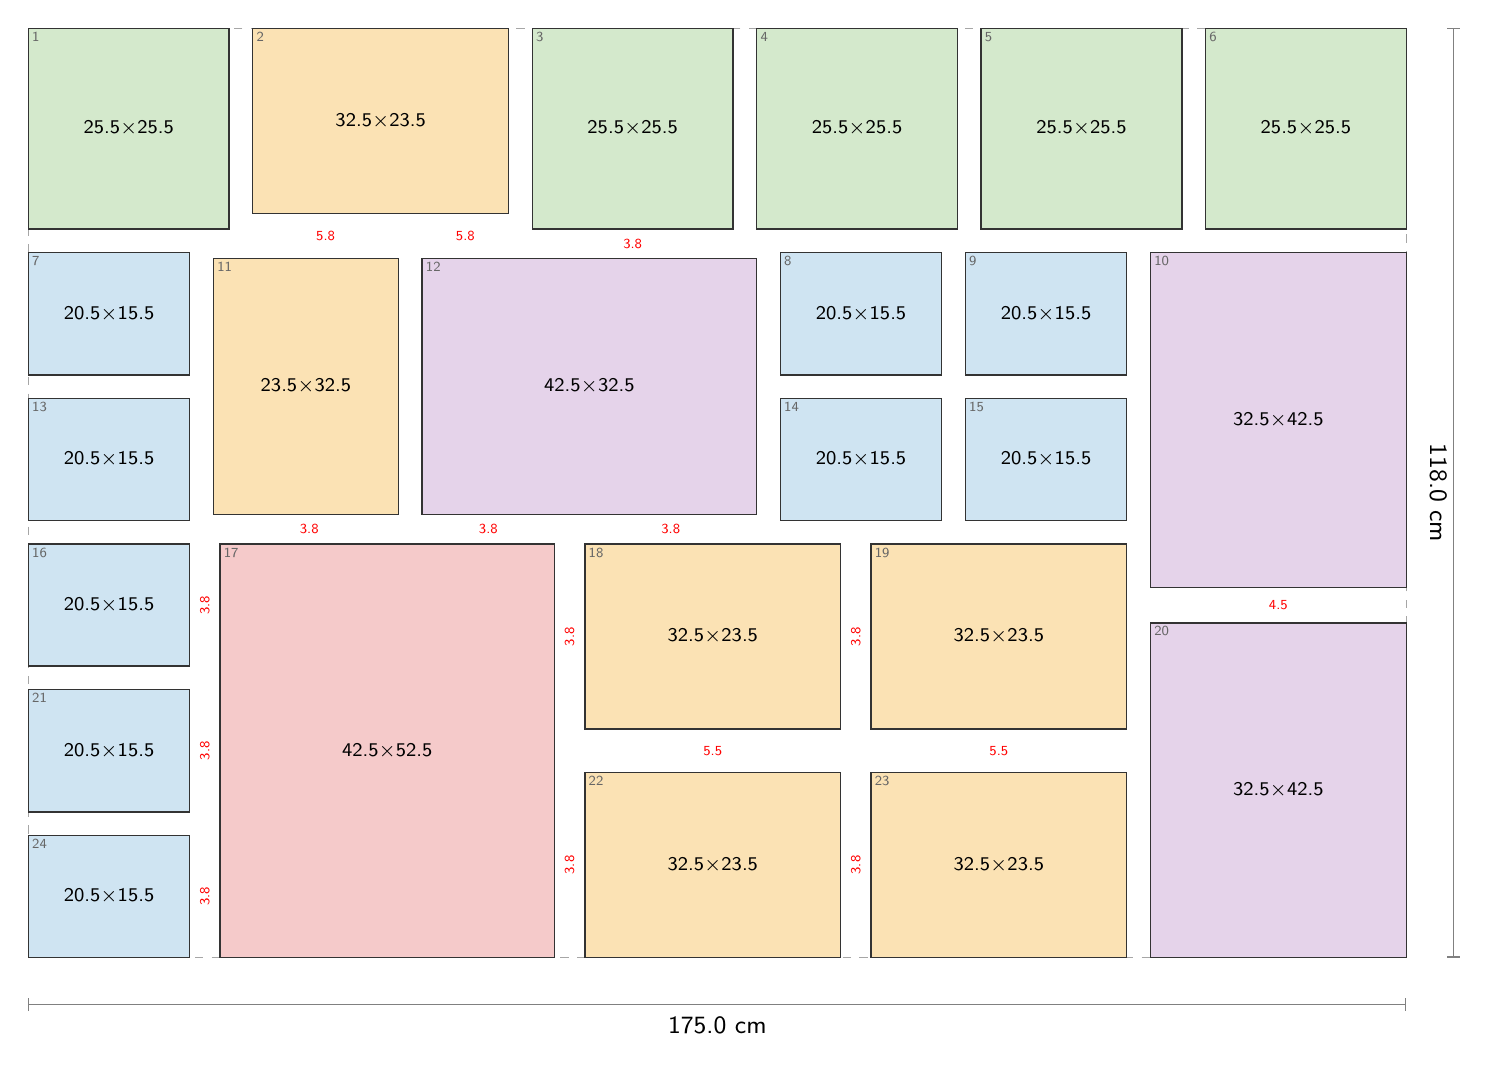
\begin{tikzpicture}[x=1mm, y=-1mm]
\draw[gray!70, dashed, line width=0.4pt] (0,0) rectangle (175.00,118.00);
\filldraw[fill=ft2, draw=black!80, line width=0.5pt] (0.00,0.00) rectangle (25.50,25.50);
\node[align=center, inner sep=0pt] at (12.75,12.75) {\scriptsize 25.5$\times$25.5};
\node[anchor=north west, inner sep=1.2pt, font=\tiny, text=black!60] at (0.00,0.00) {1};
\filldraw[fill=ft1, draw=black!80, line width=0.5pt] (28.50,0.00) rectangle (61.00,23.50);
\node[align=center, inner sep=0pt] at (44.75,11.75) {\scriptsize 32.5$\times$23.5};
\node[anchor=north west, inner sep=1.2pt, font=\tiny, text=black!60] at (28.50,0.00) {2};
\filldraw[fill=ft2, draw=black!80, line width=0.5pt] (64.00,0.00) rectangle (89.50,25.50);
\node[align=center, inner sep=0pt] at (76.75,12.75) {\scriptsize 25.5$\times$25.5};
\node[anchor=north west, inner sep=1.2pt, font=\tiny, text=black!60] at (64.00,0.00) {3};
\filldraw[fill=ft2, draw=black!80, line width=0.5pt] (92.50,0.00) rectangle (118.00,25.50);
\node[align=center, inner sep=0pt] at (105.25,12.75) {\scriptsize 25.5$\times$25.5};
\node[anchor=north west, inner sep=1.2pt, font=\tiny, text=black!60] at (92.50,0.00) {4};
\filldraw[fill=ft2, draw=black!80, line width=0.5pt] (121.00,0.00) rectangle (146.50,25.50);
\node[align=center, inner sep=0pt] at (133.75,12.75) {\scriptsize 25.5$\times$25.5};
\node[anchor=north west, inner sep=1.2pt, font=\tiny, text=black!60] at (121.00,0.00) {5};
\filldraw[fill=ft2, draw=black!80, line width=0.5pt] (149.50,0.00) rectangle (175.00,25.50);
\node[align=center, inner sep=0pt] at (162.25,12.75) {\scriptsize 25.5$\times$25.5};
\node[anchor=north west, inner sep=1.2pt, font=\tiny, text=black!60] at (149.50,0.00) {6};
\filldraw[fill=ft0, draw=black!80, line width=0.5pt] (0.00,28.50) rectangle (20.50,44.00);
\node[align=center, inner sep=0pt] at (10.25,36.25) {\scriptsize 20.5$\times$15.5};
\node[anchor=north west, inner sep=1.2pt, font=\tiny, text=black!60] at (0.00,28.50) {7};
\filldraw[fill=ft0, draw=black!80, line width=0.5pt] (95.50,28.50) rectangle (116.00,44.00);
\node[align=center, inner sep=0pt] at (105.75,36.25) {\scriptsize 20.5$\times$15.5};
\node[anchor=north west, inner sep=1.2pt, font=\tiny, text=black!60] at (95.50,28.50) {8};
\filldraw[fill=ft0, draw=black!80, line width=0.5pt] (119.00,28.50) rectangle (139.50,44.00);
\node[align=center, inner sep=0pt] at (129.25,36.25) {\scriptsize 20.5$\times$15.5};
\node[anchor=north west, inner sep=1.2pt, font=\tiny, text=black!60] at (119.00,28.50) {9};
\filldraw[fill=ft3, draw=black!80, line width=0.5pt] (142.50,28.50) rectangle (175.00,71.00);
\node[align=center, inner sep=0pt] at (158.75,49.75) {\scriptsize 32.5$\times$42.5};
\node[anchor=north west, inner sep=1.2pt, font=\tiny, text=black!60] at (142.50,28.50) {10};
\filldraw[fill=ft1, draw=black!80, line width=0.5pt] (23.50,29.25) rectangle (47.00,61.75);
\node[align=center, inner sep=0pt] at (35.25,45.50) {\scriptsize 23.5$\times$32.5};
\node[anchor=north west, inner sep=1.2pt, font=\tiny, text=black!60] at (23.50,29.25) {11};
\filldraw[fill=ft3, draw=black!80, line width=0.5pt] (50.00,29.25) rectangle (92.50,61.75);
\node[align=center, inner sep=0pt] at (71.25,45.50) {\scriptsize 42.5$\times$32.5};
\node[anchor=north west, inner sep=1.2pt, font=\tiny, text=black!60] at (50.00,29.25) {12};
\filldraw[fill=ft0, draw=black!80, line width=0.5pt] (0.00,47.00) rectangle (20.50,62.50);
\node[align=center, inner sep=0pt] at (10.25,54.75) {\scriptsize 20.5$\times$15.5};
\node[anchor=north west, inner sep=1.2pt, font=\tiny, text=black!60] at (0.00,47.00) {13};
\filldraw[fill=ft0, draw=black!80, line width=0.5pt] (95.50,47.00) rectangle (116.00,62.50);
\node[align=center, inner sep=0pt] at (105.75,54.75) {\scriptsize 20.5$\times$15.5};
\node[anchor=north west, inner sep=1.2pt, font=\tiny, text=black!60] at (95.50,47.00) {14};
\filldraw[fill=ft0, draw=black!80, line width=0.5pt] (119.00,47.00) rectangle (139.50,62.50);
\node[align=center, inner sep=0pt] at (129.25,54.75) {\scriptsize 20.5$\times$15.5};
\node[anchor=north west, inner sep=1.2pt, font=\tiny, text=black!60] at (119.00,47.00) {15};
\filldraw[fill=ft0, draw=black!80, line width=0.5pt] (0.00,65.50) rectangle (20.50,81.00);
\node[align=center, inner sep=0pt] at (10.25,73.25) {\scriptsize 20.5$\times$15.5};
\node[anchor=north west, inner sep=1.2pt, font=\tiny, text=black!60] at (0.00,65.50) {16};
\filldraw[fill=ft4, draw=black!80, line width=0.5pt] (24.33,65.50) rectangle (66.83,118.00);
\node[align=center, inner sep=0pt] at (45.58,91.75) {\scriptsize 42.5$\times$52.5};
\node[anchor=north west, inner sep=1.2pt, font=\tiny, text=black!60] at (24.33,65.50) {17};
\filldraw[fill=ft1, draw=black!80, line width=0.5pt] (70.67,65.50) rectangle (103.17,89.00);
\node[align=center, inner sep=0pt] at (86.92,77.25) {\scriptsize 32.5$\times$23.5};
\node[anchor=north west, inner sep=1.2pt, font=\tiny, text=black!60] at (70.67,65.50) {18};
\filldraw[fill=ft1, draw=black!80, line width=0.5pt] (107.00,65.50) rectangle (139.50,89.00);
\node[align=center, inner sep=0pt] at (123.25,77.25) {\scriptsize 32.5$\times$23.5};
\node[anchor=north west, inner sep=1.2pt, font=\tiny, text=black!60] at (107.00,65.50) {19};
\filldraw[fill=ft3, draw=black!80, line width=0.5pt] (142.50,75.50) rectangle (175.00,118.00);
\node[align=center, inner sep=0pt] at (158.75,96.75) {\scriptsize 32.5$\times$42.5};
\node[anchor=north west, inner sep=1.2pt, font=\tiny, text=black!60] at (142.50,75.50) {20};
\filldraw[fill=ft0, draw=black!80, line width=0.5pt] (0.00,84.00) rectangle (20.50,99.50);
\node[align=center, inner sep=0pt] at (10.25,91.75) {\scriptsize 20.5$\times$15.5};
\node[anchor=north west, inner sep=1.2pt, font=\tiny, text=black!60] at (0.00,84.00) {21};
\filldraw[fill=ft1, draw=black!80, line width=0.5pt] (70.67,94.50) rectangle (103.17,118.00);
\node[align=center, inner sep=0pt] at (86.92,106.25) {\scriptsize 32.5$\times$23.5};
\node[anchor=north west, inner sep=1.2pt, font=\tiny, text=black!60] at (70.67,94.50) {22};
\filldraw[fill=ft1, draw=black!80, line width=0.5pt] (107.00,94.50) rectangle (139.50,118.00);
\node[align=center, inner sep=0pt] at (123.25,106.25) {\scriptsize 32.5$\times$23.5};
\node[anchor=north west, inner sep=1.2pt, font=\tiny, text=black!60] at (107.00,94.50) {23};
\filldraw[fill=ft0, draw=black!80, line width=0.5pt] (0.00,102.50) rectangle (20.50,118.00);
\node[align=center, inner sep=0pt] at (10.25,110.25) {\scriptsize 20.5$\times$15.5};
\node[anchor=north west, inner sep=1.2pt, font=\tiny, text=black!60] at (0.00,102.50) {24};
\node[font=\tiny, text=red, fill=white, inner sep=0.3pt] at (37.75,26.38) {5.8};
\node[font=\tiny, text=red, fill=white, inner sep=0.3pt] at (55.50,26.38) {5.8};
\node[font=\tiny, text=red, fill=white, inner sep=0.3pt] at (76.75,27.38) {3.8};
\node[font=\tiny, text=red, fill=white, inner sep=0.3pt] at (158.75,73.25) {4.5};
\node[font=\tiny, text=red, fill=white, inner sep=0.3pt] at (35.67,63.62) {3.8};
\node[font=\tiny, text=red, fill=white, inner sep=0.3pt] at (58.42,63.62) {3.8};
\node[font=\tiny, text=red, fill=white, inner sep=0.3pt] at (81.58,63.62) {3.8};
\node[font=\tiny, text=red, fill=white, inner sep=0.3pt, rotate=90] at (22.42,73.25) {3.8};
\node[font=\tiny, text=red, fill=white, inner sep=0.3pt, rotate=90] at (68.75,77.25) {3.8};
\node[font=\tiny, text=red, fill=white, inner sep=0.3pt, rotate=90] at (68.75,106.25) {3.8};
\node[font=\tiny, text=red, fill=white, inner sep=0.3pt, rotate=90] at (105.08,77.25) {3.8};
\node[font=\tiny, text=red, fill=white, inner sep=0.3pt] at (86.92,91.75) {5.5};
\node[font=\tiny, text=red, fill=white, inner sep=0.3pt] at (123.25,91.75) {5.5};
\node[font=\tiny, text=red, fill=white, inner sep=0.3pt, rotate=90] at (22.42,91.75) {3.8};
\node[font=\tiny, text=red, fill=white, inner sep=0.3pt, rotate=90] at (105.08,106.25) {3.8};
\node[font=\tiny, text=red, fill=white, inner sep=0.3pt, rotate=90] at (22.42,110.25) {3.8};
\draw[Bar-Bar, gray] (0,124.00) -- (175.00,124.00) node[midway, below=1pt, font=\small, text=black] {175.0 cm};
\draw[Bar-Bar, gray] (181.00,0) -- (181.00,118.00) node[midway, right=1pt, font=\small, text=black, rotate=-90, anchor=north] {118.0 cm};
\end{tikzpicture}\\[4pt]
{\scriptsize Scale 1:10 (1 mm = 1 cm). Red numbers mark gaps that deviate from the nominal gap by more than 0.25 cm. Small grey numbers index the coordinate table.}
\end{minipage}\hfill
\begin{minipage}[t]{0.25\textwidth}\vspace{0pt}
\small
\begin{tabular}{@{}l l@{}}
\toprule
Outer size & 175.0 $\times$ 118.0 cm \\
Nominal gap & 3 cm \\
Actual gaps & 3.0 -- 5.8 cm \\
Max.\ deviation & 2.8 cm \\
Mean deviation & 0.45 cm \\
Border notches & right 4 cm \\
Corners filled & 4 / 4 \\
Frames used & 24 of 28 \\
\bottomrule
\end{tabular}

\vspace{8pt}
\scriptsize
\begin{tabular}{@{}c l l r r@{}}
\toprule
 & outer w $\times$ h (cm) & & used & have \\
\midrule
\tikz[baseline=-0.6ex]\fill[ft0,draw=black!60] (0,0) rectangle (1.2ex,1.2ex); & 20.5$\times$15.5 & L & 9 & 9 \\
\tikz[baseline=-0.6ex]\fill[ft0,draw=black!60] (0,0) rectangle (1.2ex,1.2ex); & 15.5$\times$20.5 & P & 0 & 2 \\
\tikz[baseline=-0.6ex]\fill[ft3,draw=black!60] (0,0) rectangle (1.2ex,1.2ex); & 32.5$\times$42.5 & P & 2 & 2 \\
\tikz[baseline=-0.6ex]\fill[ft3,draw=black!60] (0,0) rectangle (1.2ex,1.2ex); & 42.5$\times$32.5 & L & 1 & 1 \\
\tikz[baseline=-0.6ex]\fill[ft1,draw=black!60] (0,0) rectangle (1.2ex,1.2ex); & 32.5$\times$23.5 & L & 5 & 5 \\
\tikz[baseline=-0.6ex]\fill[ft1,draw=black!60] (0,0) rectangle (1.2ex,1.2ex); & 23.5$\times$32.5 & P & 1 & 1 \\
\tikz[baseline=-0.6ex]\fill[ft2,draw=black!60] (0,0) rectangle (1.2ex,1.2ex); & 25.5$\times$25.5 &  & 5 & 5 \\
\tikz[baseline=-0.6ex]\fill[ft4,draw=black!60] (0,0) rectangle (1.2ex,1.2ex); & 42.5$\times$52.5 & P & 1 & 1 \\
\tikz[baseline=-0.6ex]\fill[ft4,draw=black!60] (0,0) rectangle (1.2ex,1.2ex); & 52.5$\times$42.5 & L & 0 & 2 \\
\bottomrule
\end{tabular}

\vspace{8pt}
{\bfseries Positions} (top-left corner, cm)\\[2pt]
\tiny
\begin{tabular}{@{}r l r r@{}}
\toprule
\# & frame w $\times$ h & x & y \\
\midrule
1 & 25.5 $\times$ 25.5 & 0.0 & 0.0 \\
2 & 32.5 $\times$ 23.5 & 28.5 & 0.0 \\
3 & 25.5 $\times$ 25.5 & 64.0 & 0.0 \\
4 & 25.5 $\times$ 25.5 & 92.5 & 0.0 \\
5 & 25.5 $\times$ 25.5 & 121.0 & 0.0 \\
6 & 25.5 $\times$ 25.5 & 149.5 & 0.0 \\
7 & 20.5 $\times$ 15.5 & 0.0 & 28.5 \\
8 & 20.5 $\times$ 15.5 & 95.5 & 28.5 \\
9 & 20.5 $\times$ 15.5 & 119.0 & 28.5 \\
10 & 32.5 $\times$ 42.5 & 142.5 & 28.5 \\
11 & 23.5 $\times$ 32.5 & 23.5 & 29.2 \\
12 & 42.5 $\times$ 32.5 & 50.0 & 29.2 \\
13 & 20.5 $\times$ 15.5 & 0.0 & 47.0 \\
14 & 20.5 $\times$ 15.5 & 95.5 & 47.0 \\
15 & 20.5 $\times$ 15.5 & 119.0 & 47.0 \\
16 & 20.5 $\times$ 15.5 & 0.0 & 65.5 \\
17 & 42.5 $\times$ 52.5 & 24.3 & 65.5 \\
18 & 32.5 $\times$ 23.5 & 70.7 & 65.5 \\
19 & 32.5 $\times$ 23.5 & 107.0 & 65.5 \\
20 & 32.5 $\times$ 42.5 & 142.5 & 75.5 \\
21 & 20.5 $\times$ 15.5 & 0.0 & 84.0 \\
22 & 32.5 $\times$ 23.5 & 70.7 & 94.5 \\
23 & 32.5 $\times$ 23.5 & 107.0 & 94.5 \\
24 & 20.5 $\times$ 15.5 & 0.0 & 102.5 \\
\bottomrule
\end{tabular}
\end{minipage}
\clearpage

\begin{minipage}[t]{0.74\textwidth}\vspace{0pt}
{\LARGE\bfseries Layout 14}\hspace{1.5em}{\large 178.5 $\times$ 126.5 cm \quad gap 3 cm \quad 24 frames}\\[8pt]
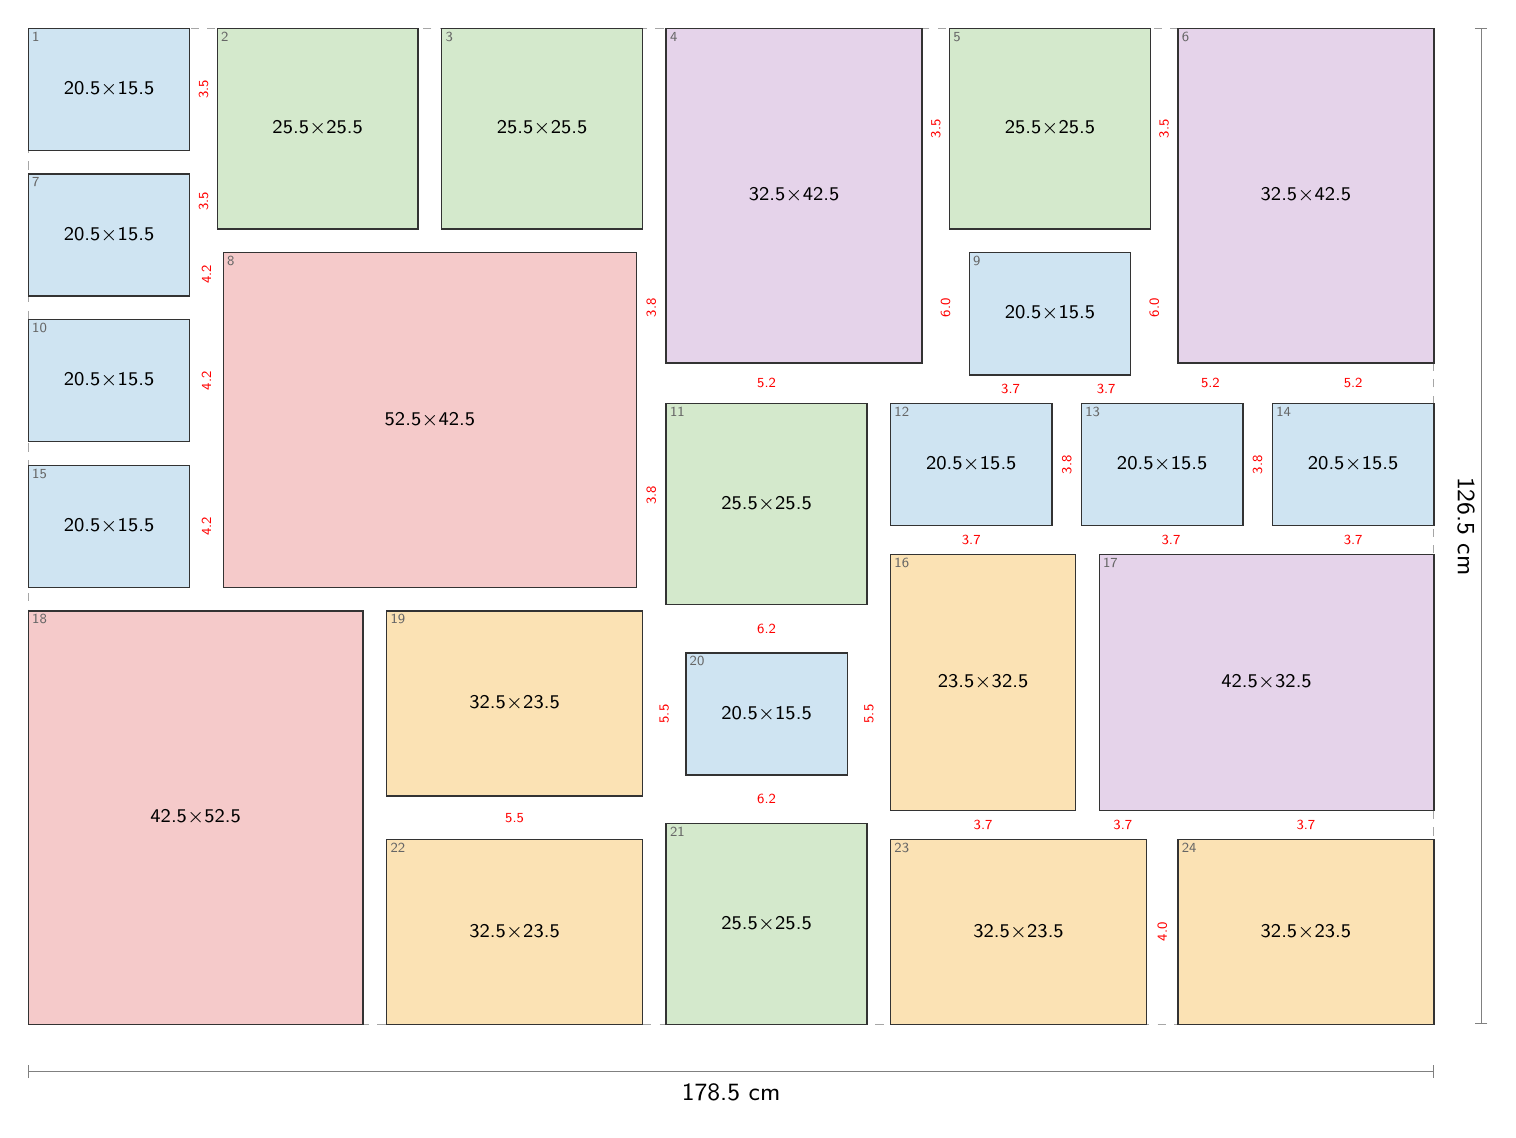
\begin{tikzpicture}[x=1mm, y=-1mm]
\draw[gray!70, dashed, line width=0.4pt] (0,0) rectangle (178.50,126.50);
\filldraw[fill=ft0, draw=black!80, line width=0.5pt] (0.00,0.00) rectangle (20.50,15.50);
\node[align=center, inner sep=0pt] at (10.25,7.75) {\scriptsize 20.5$\times$15.5};
\node[anchor=north west, inner sep=1.2pt, font=\tiny, text=black!60] at (0.00,0.00) {1};
\filldraw[fill=ft2, draw=black!80, line width=0.5pt] (24.00,0.00) rectangle (49.50,25.50);
\node[align=center, inner sep=0pt] at (36.75,12.75) {\scriptsize 25.5$\times$25.5};
\node[anchor=north west, inner sep=1.2pt, font=\tiny, text=black!60] at (24.00,0.00) {2};
\filldraw[fill=ft2, draw=black!80, line width=0.5pt] (52.50,0.00) rectangle (78.00,25.50);
\node[align=center, inner sep=0pt] at (65.25,12.75) {\scriptsize 25.5$\times$25.5};
\node[anchor=north west, inner sep=1.2pt, font=\tiny, text=black!60] at (52.50,0.00) {3};
\filldraw[fill=ft3, draw=black!80, line width=0.5pt] (81.00,0.00) rectangle (113.50,42.50);
\node[align=center, inner sep=0pt] at (97.25,21.25) {\scriptsize 32.5$\times$42.5};
\node[anchor=north west, inner sep=1.2pt, font=\tiny, text=black!60] at (81.00,0.00) {4};
\filldraw[fill=ft2, draw=black!80, line width=0.5pt] (117.00,0.00) rectangle (142.50,25.50);
\node[align=center, inner sep=0pt] at (129.75,12.75) {\scriptsize 25.5$\times$25.5};
\node[anchor=north west, inner sep=1.2pt, font=\tiny, text=black!60] at (117.00,0.00) {5};
\filldraw[fill=ft3, draw=black!80, line width=0.5pt] (146.00,0.00) rectangle (178.50,42.50);
\node[align=center, inner sep=0pt] at (162.25,21.25) {\scriptsize 32.5$\times$42.5};
\node[anchor=north west, inner sep=1.2pt, font=\tiny, text=black!60] at (146.00,0.00) {6};
\filldraw[fill=ft0, draw=black!80, line width=0.5pt] (0.00,18.50) rectangle (20.50,34.00);
\node[align=center, inner sep=0pt] at (10.25,26.25) {\scriptsize 20.5$\times$15.5};
\node[anchor=north west, inner sep=1.2pt, font=\tiny, text=black!60] at (0.00,18.50) {7};
\filldraw[fill=ft4, draw=black!80, line width=0.5pt] (24.75,28.50) rectangle (77.25,71.00);
\node[align=center, inner sep=0pt] at (51.00,49.75) {\scriptsize 52.5$\times$42.5};
\node[anchor=north west, inner sep=1.2pt, font=\tiny, text=black!60] at (24.75,28.50) {8};
\filldraw[fill=ft0, draw=black!80, line width=0.5pt] (119.50,28.50) rectangle (140.00,44.00);
\node[align=center, inner sep=0pt] at (129.75,36.25) {\scriptsize 20.5$\times$15.5};
\node[anchor=north west, inner sep=1.2pt, font=\tiny, text=black!60] at (119.50,28.50) {9};
\filldraw[fill=ft0, draw=black!80, line width=0.5pt] (0.00,37.00) rectangle (20.50,52.50);
\node[align=center, inner sep=0pt] at (10.25,44.75) {\scriptsize 20.5$\times$15.5};
\node[anchor=north west, inner sep=1.2pt, font=\tiny, text=black!60] at (0.00,37.00) {10};
\filldraw[fill=ft2, draw=black!80, line width=0.5pt] (81.00,47.67) rectangle (106.50,73.17);
\node[align=center, inner sep=0pt] at (93.75,60.42) {\scriptsize 25.5$\times$25.5};
\node[anchor=north west, inner sep=1.2pt, font=\tiny, text=black!60] at (81.00,47.67) {11};
\filldraw[fill=ft0, draw=black!80, line width=0.5pt] (109.50,47.67) rectangle (130.00,63.17);
\node[align=center, inner sep=0pt] at (119.75,55.42) {\scriptsize 20.5$\times$15.5};
\node[anchor=north west, inner sep=1.2pt, font=\tiny, text=black!60] at (109.50,47.67) {12};
\filldraw[fill=ft0, draw=black!80, line width=0.5pt] (133.75,47.67) rectangle (154.25,63.17);
\node[align=center, inner sep=0pt] at (144.00,55.42) {\scriptsize 20.5$\times$15.5};
\node[anchor=north west, inner sep=1.2pt, font=\tiny, text=black!60] at (133.75,47.67) {13};
\filldraw[fill=ft0, draw=black!80, line width=0.5pt] (158.00,47.67) rectangle (178.50,63.17);
\node[align=center, inner sep=0pt] at (168.25,55.42) {\scriptsize 20.5$\times$15.5};
\node[anchor=north west, inner sep=1.2pt, font=\tiny, text=black!60] at (158.00,47.67) {14};
\filldraw[fill=ft0, draw=black!80, line width=0.5pt] (0.00,55.50) rectangle (20.50,71.00);
\node[align=center, inner sep=0pt] at (10.25,63.25) {\scriptsize 20.5$\times$15.5};
\node[anchor=north west, inner sep=1.2pt, font=\tiny, text=black!60] at (0.00,55.50) {15};
\filldraw[fill=ft1, draw=black!80, line width=0.5pt] (109.50,66.83) rectangle (133.00,99.33);
\node[align=center, inner sep=0pt] at (121.25,83.08) {\scriptsize 23.5$\times$32.5};
\node[anchor=north west, inner sep=1.2pt, font=\tiny, text=black!60] at (109.50,66.83) {16};
\filldraw[fill=ft3, draw=black!80, line width=0.5pt] (136.00,66.83) rectangle (178.50,99.33);
\node[align=center, inner sep=0pt] at (157.25,83.08) {\scriptsize 42.5$\times$32.5};
\node[anchor=north west, inner sep=1.2pt, font=\tiny, text=black!60] at (136.00,66.83) {17};
\filldraw[fill=ft4, draw=black!80, line width=0.5pt] (0.00,74.00) rectangle (42.50,126.50);
\node[align=center, inner sep=0pt] at (21.25,100.25) {\scriptsize 42.5$\times$52.5};
\node[anchor=north west, inner sep=1.2pt, font=\tiny, text=black!60] at (0.00,74.00) {18};
\filldraw[fill=ft1, draw=black!80, line width=0.5pt] (45.50,74.00) rectangle (78.00,97.50);
\node[align=center, inner sep=0pt] at (61.75,85.75) {\scriptsize 32.5$\times$23.5};
\node[anchor=north west, inner sep=1.2pt, font=\tiny, text=black!60] at (45.50,74.00) {19};
\filldraw[fill=ft0, draw=black!80, line width=0.5pt] (83.50,79.33) rectangle (104.00,94.83);
\node[align=center, inner sep=0pt] at (93.75,87.08) {\scriptsize 20.5$\times$15.5};
\node[anchor=north west, inner sep=1.2pt, font=\tiny, text=black!60] at (83.50,79.33) {20};
\filldraw[fill=ft2, draw=black!80, line width=0.5pt] (81.00,101.00) rectangle (106.50,126.50);
\node[align=center, inner sep=0pt] at (93.75,113.75) {\scriptsize 25.5$\times$25.5};
\node[anchor=north west, inner sep=1.2pt, font=\tiny, text=black!60] at (81.00,101.00) {21};
\filldraw[fill=ft1, draw=black!80, line width=0.5pt] (45.50,103.00) rectangle (78.00,126.50);
\node[align=center, inner sep=0pt] at (61.75,114.75) {\scriptsize 32.5$\times$23.5};
\node[anchor=north west, inner sep=1.2pt, font=\tiny, text=black!60] at (45.50,103.00) {22};
\filldraw[fill=ft1, draw=black!80, line width=0.5pt] (109.50,103.00) rectangle (142.00,126.50);
\node[align=center, inner sep=0pt] at (125.75,114.75) {\scriptsize 32.5$\times$23.5};
\node[anchor=north west, inner sep=1.2pt, font=\tiny, text=black!60] at (109.50,103.00) {23};
\filldraw[fill=ft1, draw=black!80, line width=0.5pt] (146.00,103.00) rectangle (178.50,126.50);
\node[align=center, inner sep=0pt] at (162.25,114.75) {\scriptsize 32.5$\times$23.5};
\node[anchor=north west, inner sep=1.2pt, font=\tiny, text=black!60] at (146.00,103.00) {24};
\node[font=\tiny, text=red, fill=white, inner sep=0.3pt, rotate=90] at (22.25,7.75) {3.5};
\node[font=\tiny, text=red, fill=white, inner sep=0.3pt, rotate=90] at (115.25,12.75) {3.5};
\node[font=\tiny, text=red, fill=white, inner sep=0.3pt, rotate=90] at (116.50,35.50) {6.0};
\node[font=\tiny, text=red, fill=white, inner sep=0.3pt] at (93.75,45.08) {5.2};
\node[font=\tiny, text=red, fill=white, inner sep=0.3pt, rotate=90] at (144.25,12.75) {3.5};
\node[font=\tiny, text=red, fill=white, inner sep=0.3pt] at (150.12,45.08) {5.2};
\node[font=\tiny, text=red, fill=white, inner sep=0.3pt] at (168.25,45.08) {5.2};
\node[font=\tiny, text=red, fill=white, inner sep=0.3pt, rotate=90] at (22.25,22.00) {3.5};
\node[font=\tiny, text=red, fill=white, inner sep=0.3pt, rotate=90] at (22.62,31.25) {4.2};
\node[font=\tiny, text=red, fill=white, inner sep=0.3pt, rotate=90] at (79.12,35.50) {3.8};
\node[font=\tiny, text=red, fill=white, inner sep=0.3pt, rotate=90] at (79.12,59.33) {3.8};
\node[font=\tiny, text=red, fill=white, inner sep=0.3pt, rotate=90] at (143.00,35.50) {6.0};
\node[font=\tiny, text=red, fill=white, inner sep=0.3pt] at (124.75,45.83) {3.7};
\node[font=\tiny, text=red, fill=white, inner sep=0.3pt] at (136.88,45.83) {3.7};
\node[font=\tiny, text=red, fill=white, inner sep=0.3pt, rotate=90] at (22.62,44.75) {4.2};
\node[font=\tiny, text=red, fill=white, inner sep=0.3pt] at (93.75,76.25) {6.2};
\node[font=\tiny, text=red, fill=white, inner sep=0.3pt, rotate=90] at (131.88,55.42) {3.8};
\node[font=\tiny, text=red, fill=white, inner sep=0.3pt] at (119.75,65.00) {3.7};
\node[font=\tiny, text=red, fill=white, inner sep=0.3pt, rotate=90] at (156.12,55.42) {3.8};
\node[font=\tiny, text=red, fill=white, inner sep=0.3pt] at (145.12,65.00) {3.7};
\node[font=\tiny, text=red, fill=white, inner sep=0.3pt] at (168.25,65.00) {3.7};
\node[font=\tiny, text=red, fill=white, inner sep=0.3pt, rotate=90] at (22.62,63.25) {4.2};
\node[font=\tiny, text=red, fill=white, inner sep=0.3pt] at (121.25,101.17) {3.7};
\node[font=\tiny, text=red, fill=white, inner sep=0.3pt] at (139.00,101.17) {3.7};
\node[font=\tiny, text=red, fill=white, inner sep=0.3pt] at (162.25,101.17) {3.7};
\node[font=\tiny, text=red, fill=white, inner sep=0.3pt, rotate=90] at (80.75,87.08) {5.5};
\node[font=\tiny, text=red, fill=white, inner sep=0.3pt] at (61.75,100.25) {5.5};
\node[font=\tiny, text=red, fill=white, inner sep=0.3pt, rotate=90] at (106.75,87.08) {5.5};
\node[font=\tiny, text=red, fill=white, inner sep=0.3pt] at (93.75,97.92) {6.2};
\node[font=\tiny, text=red, fill=white, inner sep=0.3pt, rotate=90] at (144.00,114.75) {4.0};
\draw[Bar-Bar, gray] (0,132.50) -- (178.50,132.50) node[midway, below=1pt, font=\small, text=black] {178.5 cm};
\draw[Bar-Bar, gray] (184.50,0) -- (184.50,126.50) node[midway, right=1pt, font=\small, text=black, rotate=-90, anchor=north] {126.5 cm};
\end{tikzpicture}\\[4pt]
{\scriptsize Scale 1:10 (1 mm = 1 cm). Red numbers mark gaps that deviate from the nominal gap by more than 0.25 cm. Small grey numbers index the coordinate table.}
\end{minipage}\hfill
\begin{minipage}[t]{0.25\textwidth}\vspace{0pt}
\small
\begin{tabular}{@{}l l@{}}
\toprule
Outer size & 178.5 $\times$ 126.5 cm \\
Nominal gap & 3 cm \\
Actual gaps & 3.0 -- 6.2 cm \\
Max.\ deviation & 3.2 cm \\
Mean deviation & 0.86 cm \\
Border notches & right 5 cm \\
Corners filled & 4 / 4 \\
Frames used & 24 of 28 \\
\bottomrule
\end{tabular}

\vspace{8pt}
\scriptsize
\begin{tabular}{@{}c l l r r@{}}
\toprule
 & outer w $\times$ h (cm) & & used & have \\
\midrule
\tikz[baseline=-0.6ex]\fill[ft0,draw=black!60] (0,0) rectangle (1.2ex,1.2ex); & 20.5$\times$15.5 & L & 9 & 9 \\
\tikz[baseline=-0.6ex]\fill[ft0,draw=black!60] (0,0) rectangle (1.2ex,1.2ex); & 15.5$\times$20.5 & P & 0 & 2 \\
\tikz[baseline=-0.6ex]\fill[ft3,draw=black!60] (0,0) rectangle (1.2ex,1.2ex); & 32.5$\times$42.5 & P & 2 & 2 \\
\tikz[baseline=-0.6ex]\fill[ft3,draw=black!60] (0,0) rectangle (1.2ex,1.2ex); & 42.5$\times$32.5 & L & 1 & 1 \\
\tikz[baseline=-0.6ex]\fill[ft1,draw=black!60] (0,0) rectangle (1.2ex,1.2ex); & 32.5$\times$23.5 & L & 4 & 5 \\
\tikz[baseline=-0.6ex]\fill[ft1,draw=black!60] (0,0) rectangle (1.2ex,1.2ex); & 23.5$\times$32.5 & P & 1 & 1 \\
\tikz[baseline=-0.6ex]\fill[ft2,draw=black!60] (0,0) rectangle (1.2ex,1.2ex); & 25.5$\times$25.5 &  & 5 & 5 \\
\tikz[baseline=-0.6ex]\fill[ft4,draw=black!60] (0,0) rectangle (1.2ex,1.2ex); & 42.5$\times$52.5 & P & 1 & 1 \\
\tikz[baseline=-0.6ex]\fill[ft4,draw=black!60] (0,0) rectangle (1.2ex,1.2ex); & 52.5$\times$42.5 & L & 1 & 2 \\
\bottomrule
\end{tabular}

\vspace{8pt}
{\bfseries Positions} (top-left corner, cm)\\[2pt]
\tiny
\begin{tabular}{@{}r l r r@{}}
\toprule
\# & frame w $\times$ h & x & y \\
\midrule
1 & 20.5 $\times$ 15.5 & 0.0 & 0.0 \\
2 & 25.5 $\times$ 25.5 & 24.0 & 0.0 \\
3 & 25.5 $\times$ 25.5 & 52.5 & 0.0 \\
4 & 32.5 $\times$ 42.5 & 81.0 & 0.0 \\
5 & 25.5 $\times$ 25.5 & 117.0 & 0.0 \\
6 & 32.5 $\times$ 42.5 & 146.0 & 0.0 \\
7 & 20.5 $\times$ 15.5 & 0.0 & 18.5 \\
8 & 52.5 $\times$ 42.5 & 24.8 & 28.5 \\
9 & 20.5 $\times$ 15.5 & 119.5 & 28.5 \\
10 & 20.5 $\times$ 15.5 & 0.0 & 37.0 \\
11 & 25.5 $\times$ 25.5 & 81.0 & 47.7 \\
12 & 20.5 $\times$ 15.5 & 109.5 & 47.7 \\
13 & 20.5 $\times$ 15.5 & 133.8 & 47.7 \\
14 & 20.5 $\times$ 15.5 & 158.0 & 47.7 \\
15 & 20.5 $\times$ 15.5 & 0.0 & 55.5 \\
16 & 23.5 $\times$ 32.5 & 109.5 & 66.8 \\
17 & 42.5 $\times$ 32.5 & 136.0 & 66.8 \\
18 & 42.5 $\times$ 52.5 & 0.0 & 74.0 \\
19 & 32.5 $\times$ 23.5 & 45.5 & 74.0 \\
20 & 20.5 $\times$ 15.5 & 83.5 & 79.3 \\
21 & 25.5 $\times$ 25.5 & 81.0 & 101.0 \\
22 & 32.5 $\times$ 23.5 & 45.5 & 103.0 \\
23 & 32.5 $\times$ 23.5 & 109.5 & 103.0 \\
24 & 32.5 $\times$ 23.5 & 146.0 & 103.0 \\
\bottomrule
\end{tabular}
\end{minipage}
\clearpage

\begin{minipage}[t]{0.74\textwidth}\vspace{0pt}
{\LARGE\bfseries Layout 15}\hspace{1.5em}{\large 189.0 $\times$ 118.0 cm \quad gap 3 cm \quad 23 frames}\\[8pt]
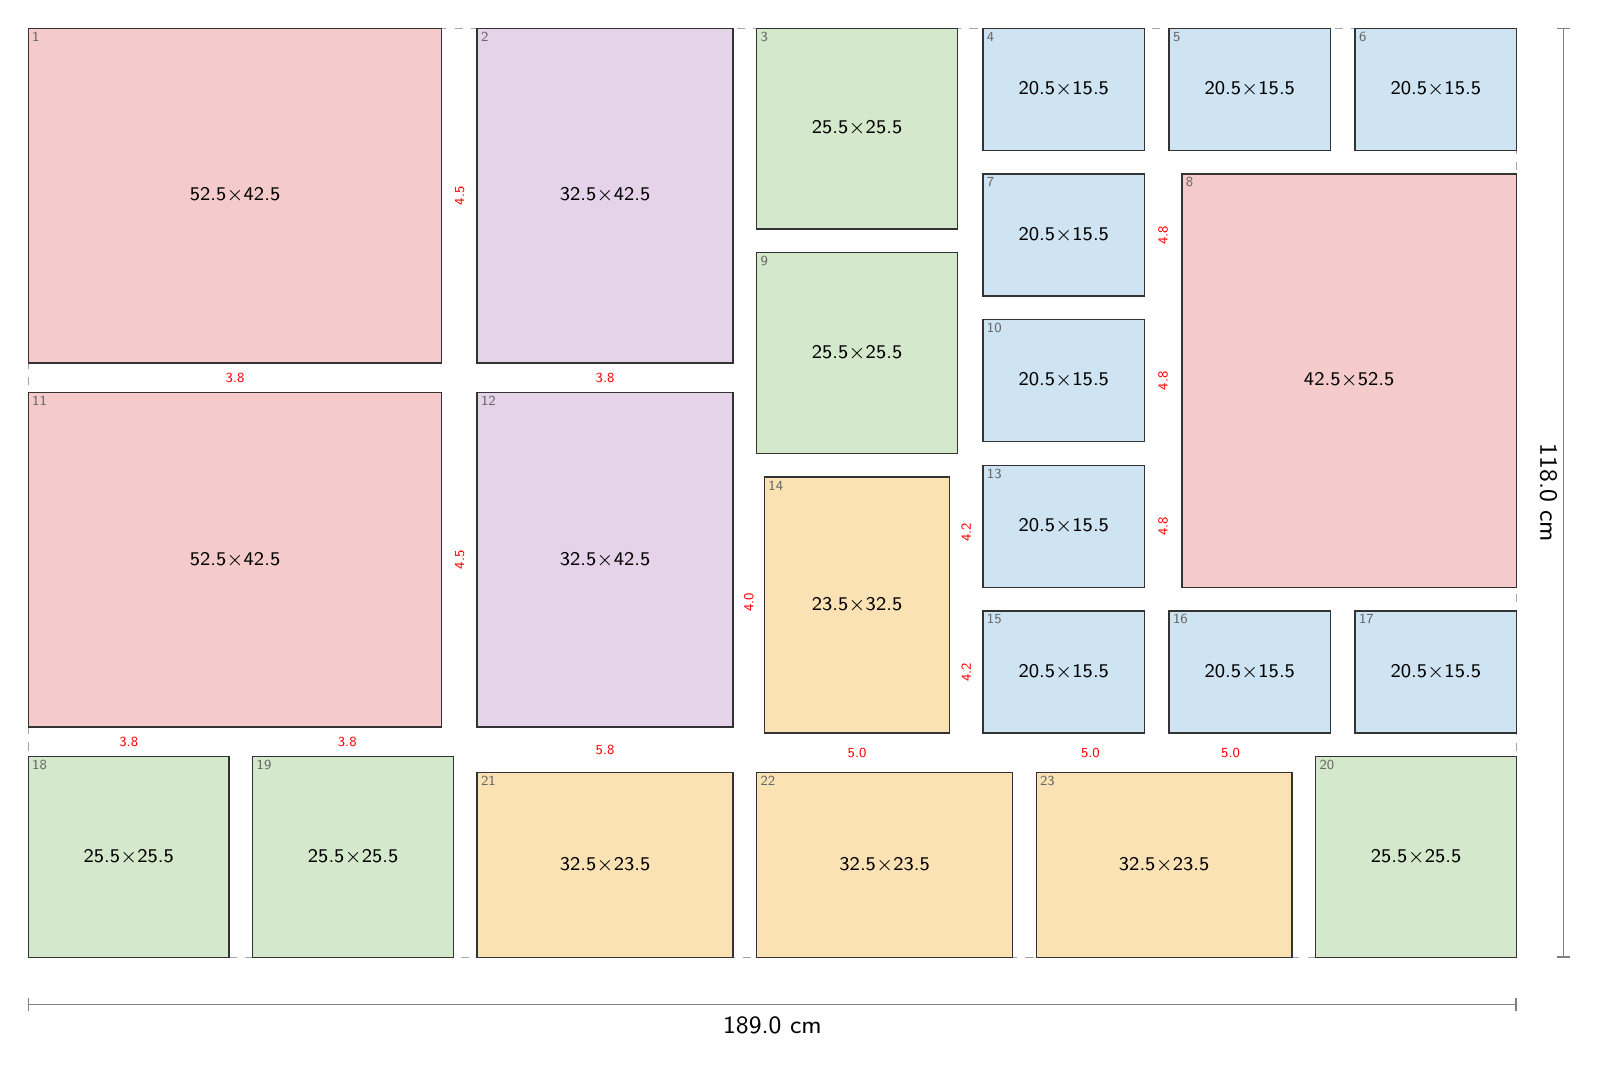
\begin{tikzpicture}[x=1mm, y=-1mm]
\draw[gray!70, dashed, line width=0.4pt] (0,0) rectangle (189.00,118.00);
\filldraw[fill=ft4, draw=black!80, line width=0.5pt] (0.00,0.00) rectangle (52.50,42.50);
\node[align=center, inner sep=0pt] at (26.25,21.25) {\scriptsize 52.5$\times$42.5};
\node[anchor=north west, inner sep=1.2pt, font=\tiny, text=black!60] at (0.00,0.00) {1};
\filldraw[fill=ft3, draw=black!80, line width=0.5pt] (57.00,0.00) rectangle (89.50,42.50);
\node[align=center, inner sep=0pt] at (73.25,21.25) {\scriptsize 32.5$\times$42.5};
\node[anchor=north west, inner sep=1.2pt, font=\tiny, text=black!60] at (57.00,0.00) {2};
\filldraw[fill=ft2, draw=black!80, line width=0.5pt] (92.50,0.00) rectangle (118.00,25.50);
\node[align=center, inner sep=0pt] at (105.25,12.75) {\scriptsize 25.5$\times$25.5};
\node[anchor=north west, inner sep=1.2pt, font=\tiny, text=black!60] at (92.50,0.00) {3};
\filldraw[fill=ft0, draw=black!80, line width=0.5pt] (121.25,0.00) rectangle (141.75,15.50);
\node[align=center, inner sep=0pt] at (131.50,7.75) {\scriptsize 20.5$\times$15.5};
\node[anchor=north west, inner sep=1.2pt, font=\tiny, text=black!60] at (121.25,0.00) {4};
\filldraw[fill=ft0, draw=black!80, line width=0.5pt] (144.88,0.00) rectangle (165.38,15.50);
\node[align=center, inner sep=0pt] at (155.12,7.75) {\scriptsize 20.5$\times$15.5};
\node[anchor=north west, inner sep=1.2pt, font=\tiny, text=black!60] at (144.88,0.00) {5};
\filldraw[fill=ft0, draw=black!80, line width=0.5pt] (168.50,0.00) rectangle (189.00,15.50);
\node[align=center, inner sep=0pt] at (178.75,7.75) {\scriptsize 20.5$\times$15.5};
\node[anchor=north west, inner sep=1.2pt, font=\tiny, text=black!60] at (168.50,0.00) {6};
\filldraw[fill=ft0, draw=black!80, line width=0.5pt] (121.25,18.50) rectangle (141.75,34.00);
\node[align=center, inner sep=0pt] at (131.50,26.25) {\scriptsize 20.5$\times$15.5};
\node[anchor=north west, inner sep=1.2pt, font=\tiny, text=black!60] at (121.25,18.50) {7};
\filldraw[fill=ft4, draw=black!80, line width=0.5pt] (146.50,18.50) rectangle (189.00,71.00);
\node[align=center, inner sep=0pt] at (167.75,44.75) {\scriptsize 42.5$\times$52.5};
\node[anchor=north west, inner sep=1.2pt, font=\tiny, text=black!60] at (146.50,18.50) {8};
\filldraw[fill=ft2, draw=black!80, line width=0.5pt] (92.50,28.50) rectangle (118.00,54.00);
\node[align=center, inner sep=0pt] at (105.25,41.25) {\scriptsize 25.5$\times$25.5};
\node[anchor=north west, inner sep=1.2pt, font=\tiny, text=black!60] at (92.50,28.50) {9};
\filldraw[fill=ft0, draw=black!80, line width=0.5pt] (121.25,37.00) rectangle (141.75,52.50);
\node[align=center, inner sep=0pt] at (131.50,44.75) {\scriptsize 20.5$\times$15.5};
\node[anchor=north west, inner sep=1.2pt, font=\tiny, text=black!60] at (121.25,37.00) {10};
\filldraw[fill=ft4, draw=black!80, line width=0.5pt] (0.00,46.25) rectangle (52.50,88.75);
\node[align=center, inner sep=0pt] at (26.25,67.50) {\scriptsize 52.5$\times$42.5};
\node[anchor=north west, inner sep=1.2pt, font=\tiny, text=black!60] at (0.00,46.25) {11};
\filldraw[fill=ft3, draw=black!80, line width=0.5pt] (57.00,46.25) rectangle (89.50,88.75);
\node[align=center, inner sep=0pt] at (73.25,67.50) {\scriptsize 32.5$\times$42.5};
\node[anchor=north west, inner sep=1.2pt, font=\tiny, text=black!60] at (57.00,46.25) {12};
\filldraw[fill=ft0, draw=black!80, line width=0.5pt] (121.25,55.50) rectangle (141.75,71.00);
\node[align=center, inner sep=0pt] at (131.50,63.25) {\scriptsize 20.5$\times$15.5};
\node[anchor=north west, inner sep=1.2pt, font=\tiny, text=black!60] at (121.25,55.50) {13};
\filldraw[fill=ft1, draw=black!80, line width=0.5pt] (93.50,57.00) rectangle (117.00,89.50);
\node[align=center, inner sep=0pt] at (105.25,73.25) {\scriptsize 23.5$\times$32.5};
\node[anchor=north west, inner sep=1.2pt, font=\tiny, text=black!60] at (93.50,57.00) {14};
\filldraw[fill=ft0, draw=black!80, line width=0.5pt] (121.25,74.00) rectangle (141.75,89.50);
\node[align=center, inner sep=0pt] at (131.50,81.75) {\scriptsize 20.5$\times$15.5};
\node[anchor=north west, inner sep=1.2pt, font=\tiny, text=black!60] at (121.25,74.00) {15};
\filldraw[fill=ft0, draw=black!80, line width=0.5pt] (144.88,74.00) rectangle (165.38,89.50);
\node[align=center, inner sep=0pt] at (155.12,81.75) {\scriptsize 20.5$\times$15.5};
\node[anchor=north west, inner sep=1.2pt, font=\tiny, text=black!60] at (144.88,74.00) {16};
\filldraw[fill=ft0, draw=black!80, line width=0.5pt] (168.50,74.00) rectangle (189.00,89.50);
\node[align=center, inner sep=0pt] at (178.75,81.75) {\scriptsize 20.5$\times$15.5};
\node[anchor=north west, inner sep=1.2pt, font=\tiny, text=black!60] at (168.50,74.00) {17};
\filldraw[fill=ft2, draw=black!80, line width=0.5pt] (0.00,92.50) rectangle (25.50,118.00);
\node[align=center, inner sep=0pt] at (12.75,105.25) {\scriptsize 25.5$\times$25.5};
\node[anchor=north west, inner sep=1.2pt, font=\tiny, text=black!60] at (0.00,92.50) {18};
\filldraw[fill=ft2, draw=black!80, line width=0.5pt] (28.50,92.50) rectangle (54.00,118.00);
\node[align=center, inner sep=0pt] at (41.25,105.25) {\scriptsize 25.5$\times$25.5};
\node[anchor=north west, inner sep=1.2pt, font=\tiny, text=black!60] at (28.50,92.50) {19};
\filldraw[fill=ft2, draw=black!80, line width=0.5pt] (163.50,92.50) rectangle (189.00,118.00);
\node[align=center, inner sep=0pt] at (176.25,105.25) {\scriptsize 25.5$\times$25.5};
\node[anchor=north west, inner sep=1.2pt, font=\tiny, text=black!60] at (163.50,92.50) {20};
\filldraw[fill=ft1, draw=black!80, line width=0.5pt] (57.00,94.50) rectangle (89.50,118.00);
\node[align=center, inner sep=0pt] at (73.25,106.25) {\scriptsize 32.5$\times$23.5};
\node[anchor=north west, inner sep=1.2pt, font=\tiny, text=black!60] at (57.00,94.50) {21};
\filldraw[fill=ft1, draw=black!80, line width=0.5pt] (92.50,94.50) rectangle (125.00,118.00);
\node[align=center, inner sep=0pt] at (108.75,106.25) {\scriptsize 32.5$\times$23.5};
\node[anchor=north west, inner sep=1.2pt, font=\tiny, text=black!60] at (92.50,94.50) {22};
\filldraw[fill=ft1, draw=black!80, line width=0.5pt] (128.00,94.50) rectangle (160.50,118.00);
\node[align=center, inner sep=0pt] at (144.25,106.25) {\scriptsize 32.5$\times$23.5};
\node[anchor=north west, inner sep=1.2pt, font=\tiny, text=black!60] at (128.00,94.50) {23};
\node[font=\tiny, text=red, fill=white, inner sep=0.3pt, rotate=90] at (54.75,21.25) {4.5};
\node[font=\tiny, text=red, fill=white, inner sep=0.3pt] at (26.25,44.38) {3.8};
\node[font=\tiny, text=red, fill=white, inner sep=0.3pt] at (73.25,44.38) {3.8};
\node[font=\tiny, text=red, fill=white, inner sep=0.3pt, rotate=90] at (144.12,26.25) {4.8};
\node[font=\tiny, text=red, fill=white, inner sep=0.3pt, rotate=90] at (144.12,44.75) {4.8};
\node[font=\tiny, text=red, fill=white, inner sep=0.3pt, rotate=90] at (54.75,67.50) {4.5};
\node[font=\tiny, text=red, fill=white, inner sep=0.3pt] at (12.75,90.62) {3.8};
\node[font=\tiny, text=red, fill=white, inner sep=0.3pt] at (40.50,90.62) {3.8};
\node[font=\tiny, text=red, fill=white, inner sep=0.3pt, rotate=90] at (91.50,72.88) {4.0};
\node[font=\tiny, text=red, fill=white, inner sep=0.3pt] at (73.25,91.62) {5.8};
\node[font=\tiny, text=red, fill=white, inner sep=0.3pt, rotate=90] at (144.12,63.25) {4.8};
\node[font=\tiny, text=red, fill=white, inner sep=0.3pt, rotate=90] at (119.12,64.00) {4.2};
\node[font=\tiny, text=red, fill=white, inner sep=0.3pt, rotate=90] at (119.12,81.75) {4.2};
\node[font=\tiny, text=red, fill=white, inner sep=0.3pt] at (105.25,92.00) {5.0};
\node[font=\tiny, text=red, fill=white, inner sep=0.3pt] at (134.88,92.00) {5.0};
\node[font=\tiny, text=red, fill=white, inner sep=0.3pt] at (152.69,92.00) {5.0};
\draw[Bar-Bar, gray] (0,124.00) -- (189.00,124.00) node[midway, below=1pt, font=\small, text=black] {189.0 cm};
\draw[Bar-Bar, gray] (195.00,0) -- (195.00,118.00) node[midway, right=1pt, font=\small, text=black, rotate=-90, anchor=north] {118.0 cm};
\end{tikzpicture}\\[4pt]
{\scriptsize Scale 1:10 (1 mm = 1 cm). Red numbers mark gaps that deviate from the nominal gap by more than 0.25 cm. Small grey numbers index the coordinate table.}
\end{minipage}\hfill
\begin{minipage}[t]{0.25\textwidth}\vspace{0pt}
\small
\begin{tabular}{@{}l l@{}}
\toprule
Outer size & 189.0 $\times$ 118.0 cm \\
Nominal gap & 3 cm \\
Actual gaps & 3.0 -- 5.8 cm \\
Max.\ deviation & 2.8 cm \\
Mean deviation & 0.58 cm \\
Border notches & top 4 cm \\
Corners filled & 4 / 4 \\
Frames used & 23 of 28 \\
\bottomrule
\end{tabular}

\vspace{8pt}
\scriptsize
\begin{tabular}{@{}c l l r r@{}}
\toprule
 & outer w $\times$ h (cm) & & used & have \\
\midrule
\tikz[baseline=-0.6ex]\fill[ft0,draw=black!60] (0,0) rectangle (1.2ex,1.2ex); & 20.5$\times$15.5 & L & 9 & 9 \\
\tikz[baseline=-0.6ex]\fill[ft0,draw=black!60] (0,0) rectangle (1.2ex,1.2ex); & 15.5$\times$20.5 & P & 0 & 2 \\
\tikz[baseline=-0.6ex]\fill[ft3,draw=black!60] (0,0) rectangle (1.2ex,1.2ex); & 32.5$\times$42.5 & P & 2 & 2 \\
\tikz[baseline=-0.6ex]\fill[ft3,draw=black!60] (0,0) rectangle (1.2ex,1.2ex); & 42.5$\times$32.5 & L & 0 & 1 \\
\tikz[baseline=-0.6ex]\fill[ft1,draw=black!60] (0,0) rectangle (1.2ex,1.2ex); & 32.5$\times$23.5 & L & 3 & 5 \\
\tikz[baseline=-0.6ex]\fill[ft1,draw=black!60] (0,0) rectangle (1.2ex,1.2ex); & 23.5$\times$32.5 & P & 1 & 1 \\
\tikz[baseline=-0.6ex]\fill[ft2,draw=black!60] (0,0) rectangle (1.2ex,1.2ex); & 25.5$\times$25.5 &  & 5 & 5 \\
\tikz[baseline=-0.6ex]\fill[ft4,draw=black!60] (0,0) rectangle (1.2ex,1.2ex); & 42.5$\times$52.5 & P & 1 & 1 \\
\tikz[baseline=-0.6ex]\fill[ft4,draw=black!60] (0,0) rectangle (1.2ex,1.2ex); & 52.5$\times$42.5 & L & 2 & 2 \\
\bottomrule
\end{tabular}

\vspace{8pt}
{\bfseries Positions} (top-left corner, cm)\\[2pt]
\tiny
\begin{tabular}{@{}r l r r@{}}
\toprule
\# & frame w $\times$ h & x & y \\
\midrule
1 & 52.5 $\times$ 42.5 & 0.0 & 0.0 \\
2 & 32.5 $\times$ 42.5 & 57.0 & 0.0 \\
3 & 25.5 $\times$ 25.5 & 92.5 & 0.0 \\
4 & 20.5 $\times$ 15.5 & 121.2 & 0.0 \\
5 & 20.5 $\times$ 15.5 & 144.9 & 0.0 \\
6 & 20.5 $\times$ 15.5 & 168.5 & 0.0 \\
7 & 20.5 $\times$ 15.5 & 121.2 & 18.5 \\
8 & 42.5 $\times$ 52.5 & 146.5 & 18.5 \\
9 & 25.5 $\times$ 25.5 & 92.5 & 28.5 \\
10 & 20.5 $\times$ 15.5 & 121.2 & 37.0 \\
11 & 52.5 $\times$ 42.5 & 0.0 & 46.2 \\
12 & 32.5 $\times$ 42.5 & 57.0 & 46.2 \\
13 & 20.5 $\times$ 15.5 & 121.2 & 55.5 \\
14 & 23.5 $\times$ 32.5 & 93.5 & 57.0 \\
15 & 20.5 $\times$ 15.5 & 121.2 & 74.0 \\
16 & 20.5 $\times$ 15.5 & 144.9 & 74.0 \\
17 & 20.5 $\times$ 15.5 & 168.5 & 74.0 \\
18 & 25.5 $\times$ 25.5 & 0.0 & 92.5 \\
19 & 25.5 $\times$ 25.5 & 28.5 & 92.5 \\
20 & 25.5 $\times$ 25.5 & 163.5 & 92.5 \\
21 & 32.5 $\times$ 23.5 & 57.0 & 94.5 \\
22 & 32.5 $\times$ 23.5 & 92.5 & 94.5 \\
23 & 32.5 $\times$ 23.5 & 128.0 & 94.5 \\
\bottomrule
\end{tabular}
\end{minipage}
\clearpage

\begin{minipage}[t]{0.74\textwidth}\vspace{0pt}
{\LARGE\bfseries Layout 16}\hspace{1.5em}{\large 181.0 $\times$ 126.5 cm \quad gap 3 cm \quad 23 frames}\\[8pt]
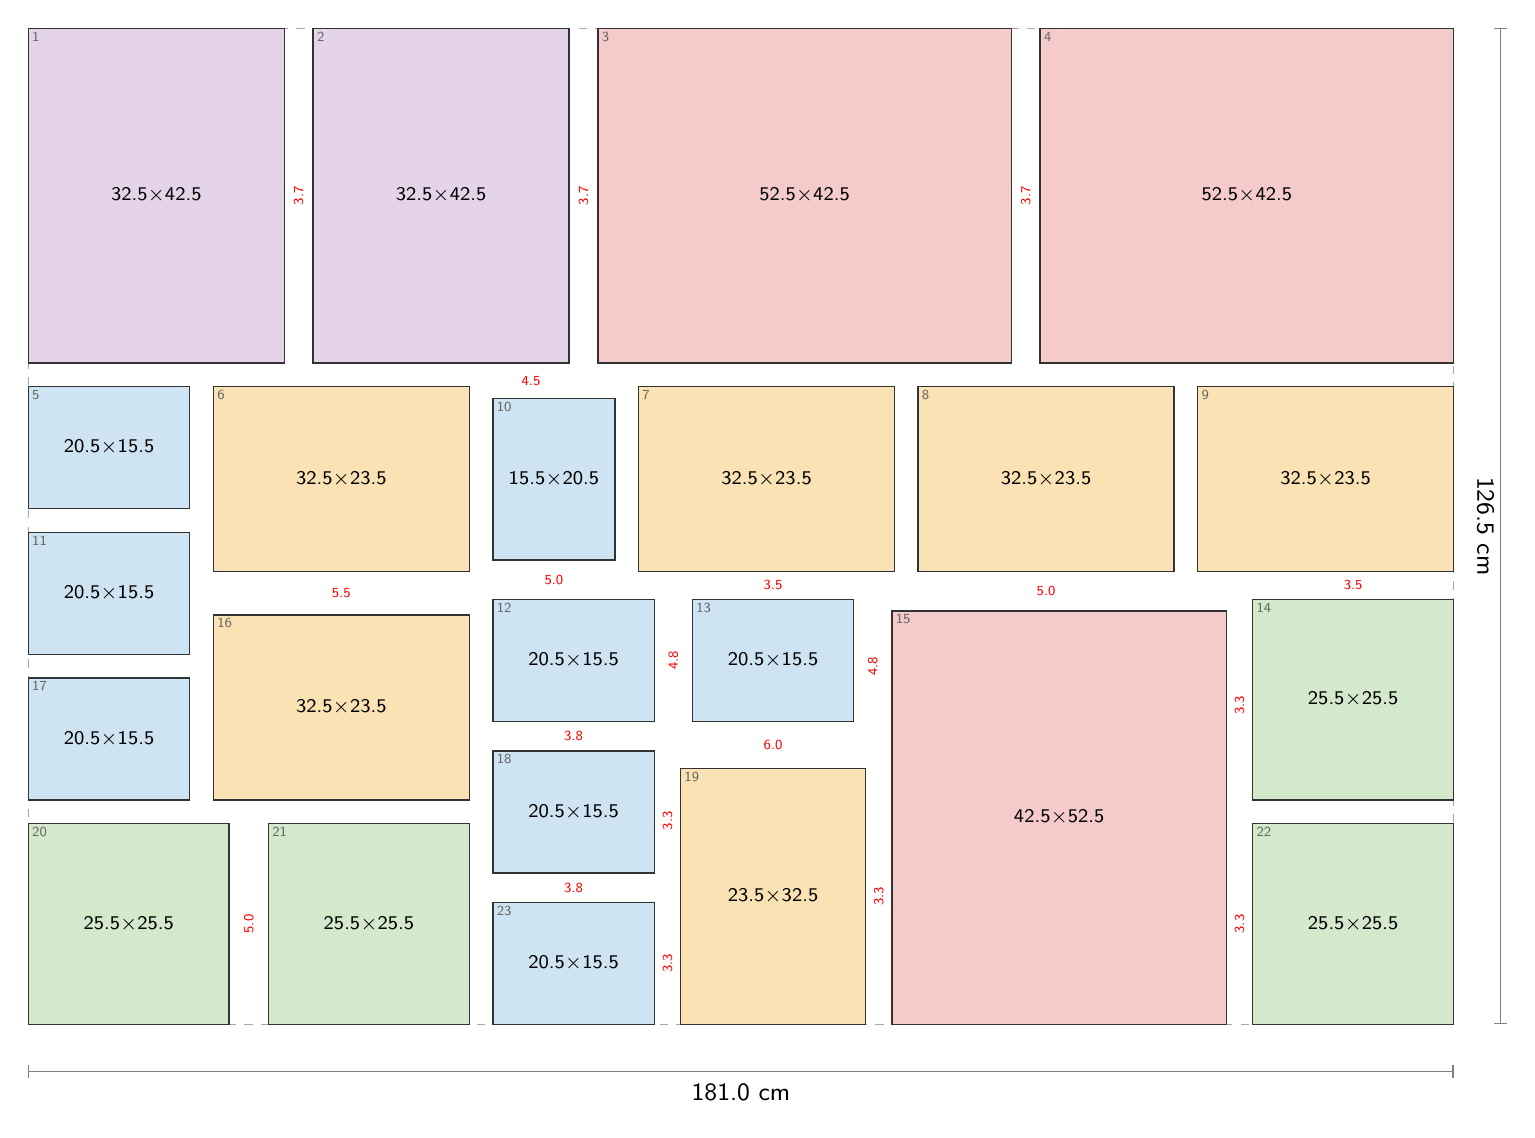
\begin{tikzpicture}[x=1mm, y=-1mm]
\draw[gray!70, dashed, line width=0.4pt] (0,0) rectangle (181.00,126.50);
\filldraw[fill=ft3, draw=black!80, line width=0.5pt] (0.00,0.00) rectangle (32.50,42.50);
\node[align=center, inner sep=0pt] at (16.25,21.25) {\scriptsize 32.5$\times$42.5};
\node[anchor=north west, inner sep=1.2pt, font=\tiny, text=black!60] at (0.00,0.00) {1};
\filldraw[fill=ft3, draw=black!80, line width=0.5pt] (36.17,0.00) rectangle (68.67,42.50);
\node[align=center, inner sep=0pt] at (52.42,21.25) {\scriptsize 32.5$\times$42.5};
\node[anchor=north west, inner sep=1.2pt, font=\tiny, text=black!60] at (36.17,0.00) {2};
\filldraw[fill=ft4, draw=black!80, line width=0.5pt] (72.33,0.00) rectangle (124.83,42.50);
\node[align=center, inner sep=0pt] at (98.58,21.25) {\scriptsize 52.5$\times$42.5};
\node[anchor=north west, inner sep=1.2pt, font=\tiny, text=black!60] at (72.33,0.00) {3};
\filldraw[fill=ft4, draw=black!80, line width=0.5pt] (128.50,0.00) rectangle (181.00,42.50);
\node[align=center, inner sep=0pt] at (154.75,21.25) {\scriptsize 52.5$\times$42.5};
\node[anchor=north west, inner sep=1.2pt, font=\tiny, text=black!60] at (128.50,0.00) {4};
\filldraw[fill=ft0, draw=black!80, line width=0.5pt] (0.00,45.50) rectangle (20.50,61.00);
\node[align=center, inner sep=0pt] at (10.25,53.25) {\scriptsize 20.5$\times$15.5};
\node[anchor=north west, inner sep=1.2pt, font=\tiny, text=black!60] at (0.00,45.50) {5};
\filldraw[fill=ft1, draw=black!80, line width=0.5pt] (23.50,45.50) rectangle (56.00,69.00);
\node[align=center, inner sep=0pt] at (39.75,57.25) {\scriptsize 32.5$\times$23.5};
\node[anchor=north west, inner sep=1.2pt, font=\tiny, text=black!60] at (23.50,45.50) {6};
\filldraw[fill=ft1, draw=black!80, line width=0.5pt] (77.50,45.50) rectangle (110.00,69.00);
\node[align=center, inner sep=0pt] at (93.75,57.25) {\scriptsize 32.5$\times$23.5};
\node[anchor=north west, inner sep=1.2pt, font=\tiny, text=black!60] at (77.50,45.50) {7};
\filldraw[fill=ft1, draw=black!80, line width=0.5pt] (113.00,45.50) rectangle (145.50,69.00);
\node[align=center, inner sep=0pt] at (129.25,57.25) {\scriptsize 32.5$\times$23.5};
\node[anchor=north west, inner sep=1.2pt, font=\tiny, text=black!60] at (113.00,45.50) {8};
\filldraw[fill=ft1, draw=black!80, line width=0.5pt] (148.50,45.50) rectangle (181.00,69.00);
\node[align=center, inner sep=0pt] at (164.75,57.25) {\scriptsize 32.5$\times$23.5};
\node[anchor=north west, inner sep=1.2pt, font=\tiny, text=black!60] at (148.50,45.50) {9};
\filldraw[fill=ft0, draw=black!80, line width=0.5pt] (59.00,47.00) rectangle (74.50,67.50);
\node[align=center, inner sep=0pt] at (66.75,57.25) {\scriptsize 15.5$\times$20.5};
\node[anchor=north west, inner sep=1.2pt, font=\tiny, text=black!60] at (59.00,47.00) {10};
\filldraw[fill=ft0, draw=black!80, line width=0.5pt] (0.00,64.00) rectangle (20.50,79.50);
\node[align=center, inner sep=0pt] at (10.25,71.75) {\scriptsize 20.5$\times$15.5};
\node[anchor=north west, inner sep=1.2pt, font=\tiny, text=black!60] at (0.00,64.00) {11};
\filldraw[fill=ft0, draw=black!80, line width=0.5pt] (59.00,72.50) rectangle (79.50,88.00);
\node[align=center, inner sep=0pt] at (69.25,80.25) {\scriptsize 20.5$\times$15.5};
\node[anchor=north west, inner sep=1.2pt, font=\tiny, text=black!60] at (59.00,72.50) {12};
\filldraw[fill=ft0, draw=black!80, line width=0.5pt] (84.33,72.50) rectangle (104.83,88.00);
\node[align=center, inner sep=0pt] at (94.58,80.25) {\scriptsize 20.5$\times$15.5};
\node[anchor=north west, inner sep=1.2pt, font=\tiny, text=black!60] at (84.33,72.50) {13};
\filldraw[fill=ft2, draw=black!80, line width=0.5pt] (155.50,72.50) rectangle (181.00,98.00);
\node[align=center, inner sep=0pt] at (168.25,85.25) {\scriptsize 25.5$\times$25.5};
\node[anchor=north west, inner sep=1.2pt, font=\tiny, text=black!60] at (155.50,72.50) {14};
\filldraw[fill=ft4, draw=black!80, line width=0.5pt] (109.67,74.00) rectangle (152.17,126.50);
\node[align=center, inner sep=0pt] at (130.92,100.25) {\scriptsize 42.5$\times$52.5};
\node[anchor=north west, inner sep=1.2pt, font=\tiny, text=black!60] at (109.67,74.00) {15};
\filldraw[fill=ft1, draw=black!80, line width=0.5pt] (23.50,74.50) rectangle (56.00,98.00);
\node[align=center, inner sep=0pt] at (39.75,86.25) {\scriptsize 32.5$\times$23.5};
\node[anchor=north west, inner sep=1.2pt, font=\tiny, text=black!60] at (23.50,74.50) {16};
\filldraw[fill=ft0, draw=black!80, line width=0.5pt] (0.00,82.50) rectangle (20.50,98.00);
\node[align=center, inner sep=0pt] at (10.25,90.25) {\scriptsize 20.5$\times$15.5};
\node[anchor=north west, inner sep=1.2pt, font=\tiny, text=black!60] at (0.00,82.50) {17};
\filldraw[fill=ft0, draw=black!80, line width=0.5pt] (59.00,91.75) rectangle (79.50,107.25);
\node[align=center, inner sep=0pt] at (69.25,99.50) {\scriptsize 20.5$\times$15.5};
\node[anchor=north west, inner sep=1.2pt, font=\tiny, text=black!60] at (59.00,91.75) {18};
\filldraw[fill=ft1, draw=black!80, line width=0.5pt] (82.83,94.00) rectangle (106.33,126.50);
\node[align=center, inner sep=0pt] at (94.58,110.25) {\scriptsize 23.5$\times$32.5};
\node[anchor=north west, inner sep=1.2pt, font=\tiny, text=black!60] at (82.83,94.00) {19};
\filldraw[fill=ft2, draw=black!80, line width=0.5pt] (0.00,101.00) rectangle (25.50,126.50);
\node[align=center, inner sep=0pt] at (12.75,113.75) {\scriptsize 25.5$\times$25.5};
\node[anchor=north west, inner sep=1.2pt, font=\tiny, text=black!60] at (0.00,101.00) {20};
\filldraw[fill=ft2, draw=black!80, line width=0.5pt] (30.50,101.00) rectangle (56.00,126.50);
\node[align=center, inner sep=0pt] at (43.25,113.75) {\scriptsize 25.5$\times$25.5};
\node[anchor=north west, inner sep=1.2pt, font=\tiny, text=black!60] at (30.50,101.00) {21};
\filldraw[fill=ft2, draw=black!80, line width=0.5pt] (155.50,101.00) rectangle (181.00,126.50);
\node[align=center, inner sep=0pt] at (168.25,113.75) {\scriptsize 25.5$\times$25.5};
\node[anchor=north west, inner sep=1.2pt, font=\tiny, text=black!60] at (155.50,101.00) {22};
\filldraw[fill=ft0, draw=black!80, line width=0.5pt] (59.00,111.00) rectangle (79.50,126.50);
\node[align=center, inner sep=0pt] at (69.25,118.75) {\scriptsize 20.5$\times$15.5};
\node[anchor=north west, inner sep=1.2pt, font=\tiny, text=black!60] at (59.00,111.00) {23};
\node[font=\tiny, text=red, fill=white, inner sep=0.3pt, rotate=90] at (34.33,21.25) {3.7};
\node[font=\tiny, text=red, fill=white, inner sep=0.3pt, rotate=90] at (70.50,21.25) {3.7};
\node[font=\tiny, text=red, fill=white, inner sep=0.3pt] at (63.83,44.75) {4.5};
\node[font=\tiny, text=red, fill=white, inner sep=0.3pt, rotate=90] at (126.67,21.25) {3.7};
\node[font=\tiny, text=red, fill=white, inner sep=0.3pt] at (39.75,71.75) {5.5};
\node[font=\tiny, text=red, fill=white, inner sep=0.3pt] at (94.58,70.75) {3.5};
\node[font=\tiny, text=red, fill=white, inner sep=0.3pt] at (129.25,71.50) {5.0};
\node[font=\tiny, text=red, fill=white, inner sep=0.3pt] at (168.25,70.75) {3.5};
\node[font=\tiny, text=red, fill=white, inner sep=0.3pt] at (66.75,70.00) {5.0};
\node[font=\tiny, text=red, fill=white, inner sep=0.3pt, rotate=90] at (81.92,80.25) {4.8};
\node[font=\tiny, text=red, fill=white, inner sep=0.3pt] at (69.25,89.88) {3.8};
\node[font=\tiny, text=red, fill=white, inner sep=0.3pt, rotate=90] at (107.25,81.00) {4.8};
\node[font=\tiny, text=red, fill=white, inner sep=0.3pt] at (94.58,91.00) {6.0};
\node[font=\tiny, text=red, fill=white, inner sep=0.3pt, rotate=90] at (153.83,86.00) {3.3};
\node[font=\tiny, text=red, fill=white, inner sep=0.3pt, rotate=90] at (153.83,113.75) {3.3};
\node[font=\tiny, text=red, fill=white, inner sep=0.3pt, rotate=90] at (81.17,100.62) {3.3};
\node[font=\tiny, text=red, fill=white, inner sep=0.3pt] at (69.25,109.12) {3.8};
\node[font=\tiny, text=red, fill=white, inner sep=0.3pt, rotate=90] at (108.00,110.25) {3.3};
\node[font=\tiny, text=red, fill=white, inner sep=0.3pt, rotate=90] at (28.00,113.75) {5.0};
\node[font=\tiny, text=red, fill=white, inner sep=0.3pt, rotate=90] at (81.17,118.75) {3.3};
\draw[Bar-Bar, gray] (0,132.50) -- (181.00,132.50) node[midway, below=1pt, font=\small, text=black] {181.0 cm};
\draw[Bar-Bar, gray] (187.00,0) -- (187.00,126.50) node[midway, right=1pt, font=\small, text=black, rotate=-90, anchor=north] {126.5 cm};
\end{tikzpicture}\\[4pt]
{\scriptsize Scale 1:10 (1 mm = 1 cm). Red numbers mark gaps that deviate from the nominal gap by more than 0.25 cm. Small grey numbers index the coordinate table.}
\end{minipage}\hfill
\begin{minipage}[t]{0.25\textwidth}\vspace{0pt}
\small
\begin{tabular}{@{}l l@{}}
\toprule
Outer size & 181.0 $\times$ 126.5 cm \\
Nominal gap & 3 cm \\
Actual gaps & 3.0 -- 6.0 cm \\
Max.\ deviation & 3.0 cm \\
Mean deviation & 0.52 cm \\
Border notches & bottom 5 cm \\
Corners filled & 4 / 4 \\
Frames used & 23 of 28 \\
\bottomrule
\end{tabular}

\vspace{8pt}
\scriptsize
\begin{tabular}{@{}c l l r r@{}}
\toprule
 & outer w $\times$ h (cm) & & used & have \\
\midrule
\tikz[baseline=-0.6ex]\fill[ft0,draw=black!60] (0,0) rectangle (1.2ex,1.2ex); & 20.5$\times$15.5 & L & 7 & 9 \\
\tikz[baseline=-0.6ex]\fill[ft0,draw=black!60] (0,0) rectangle (1.2ex,1.2ex); & 15.5$\times$20.5 & P & 1 & 2 \\
\tikz[baseline=-0.6ex]\fill[ft3,draw=black!60] (0,0) rectangle (1.2ex,1.2ex); & 32.5$\times$42.5 & P & 2 & 2 \\
\tikz[baseline=-0.6ex]\fill[ft3,draw=black!60] (0,0) rectangle (1.2ex,1.2ex); & 42.5$\times$32.5 & L & 0 & 1 \\
\tikz[baseline=-0.6ex]\fill[ft1,draw=black!60] (0,0) rectangle (1.2ex,1.2ex); & 32.5$\times$23.5 & L & 5 & 5 \\
\tikz[baseline=-0.6ex]\fill[ft1,draw=black!60] (0,0) rectangle (1.2ex,1.2ex); & 23.5$\times$32.5 & P & 1 & 1 \\
\tikz[baseline=-0.6ex]\fill[ft2,draw=black!60] (0,0) rectangle (1.2ex,1.2ex); & 25.5$\times$25.5 &  & 4 & 5 \\
\tikz[baseline=-0.6ex]\fill[ft4,draw=black!60] (0,0) rectangle (1.2ex,1.2ex); & 42.5$\times$52.5 & P & 1 & 1 \\
\tikz[baseline=-0.6ex]\fill[ft4,draw=black!60] (0,0) rectangle (1.2ex,1.2ex); & 52.5$\times$42.5 & L & 2 & 2 \\
\bottomrule
\end{tabular}

\vspace{8pt}
{\bfseries Positions} (top-left corner, cm)\\[2pt]
\tiny
\begin{tabular}{@{}r l r r@{}}
\toprule
\# & frame w $\times$ h & x & y \\
\midrule
1 & 32.5 $\times$ 42.5 & 0.0 & 0.0 \\
2 & 32.5 $\times$ 42.5 & 36.2 & 0.0 \\
3 & 52.5 $\times$ 42.5 & 72.3 & 0.0 \\
4 & 52.5 $\times$ 42.5 & 128.5 & 0.0 \\
5 & 20.5 $\times$ 15.5 & 0.0 & 45.5 \\
6 & 32.5 $\times$ 23.5 & 23.5 & 45.5 \\
7 & 32.5 $\times$ 23.5 & 77.5 & 45.5 \\
8 & 32.5 $\times$ 23.5 & 113.0 & 45.5 \\
9 & 32.5 $\times$ 23.5 & 148.5 & 45.5 \\
10 & 15.5 $\times$ 20.5 & 59.0 & 47.0 \\
11 & 20.5 $\times$ 15.5 & 0.0 & 64.0 \\
12 & 20.5 $\times$ 15.5 & 59.0 & 72.5 \\
13 & 20.5 $\times$ 15.5 & 84.3 & 72.5 \\
14 & 25.5 $\times$ 25.5 & 155.5 & 72.5 \\
15 & 42.5 $\times$ 52.5 & 109.7 & 74.0 \\
16 & 32.5 $\times$ 23.5 & 23.5 & 74.5 \\
17 & 20.5 $\times$ 15.5 & 0.0 & 82.5 \\
18 & 20.5 $\times$ 15.5 & 59.0 & 91.8 \\
19 & 23.5 $\times$ 32.5 & 82.8 & 94.0 \\
20 & 25.5 $\times$ 25.5 & 0.0 & 101.0 \\
21 & 25.5 $\times$ 25.5 & 30.5 & 101.0 \\
22 & 25.5 $\times$ 25.5 & 155.5 & 101.0 \\
23 & 20.5 $\times$ 15.5 & 59.0 & 111.0 \\
\bottomrule
\end{tabular}
\end{minipage}
\clearpage

\end{document}
